% !TeX spellcheck = en_GB
% %%% ***************** CHAPTER RESULTS ***************** %%%

%%%%%%%%%%%%%%%%%%%%%%%%%%%%%%%%%%%%%%%%%%%%%%%%%%%%%%%%%%%%%%%%%%%%%%%%%
%%%%%%%% surface %%%%%%%%%%%%%%
% !TeX spellcheck = en_GB

%%%%%%%%%%%%%%%%%%%%%%%%%%%%%%%%%%%%%%%%%%%%%%%%%%%%%%%%%%%%%%%%%%%%%%%%%%
%%%%%%%%% Observation agreement %%%%%%%%%%%%%%
\section{Agreement between surface observations} 
%%%%%%% image scatter obs ret %%%%%%%%%%%%%%%%
\begin{figure}[t]
	\centering
    \begin{subfigure}[b]{0.38\textwidth}
    	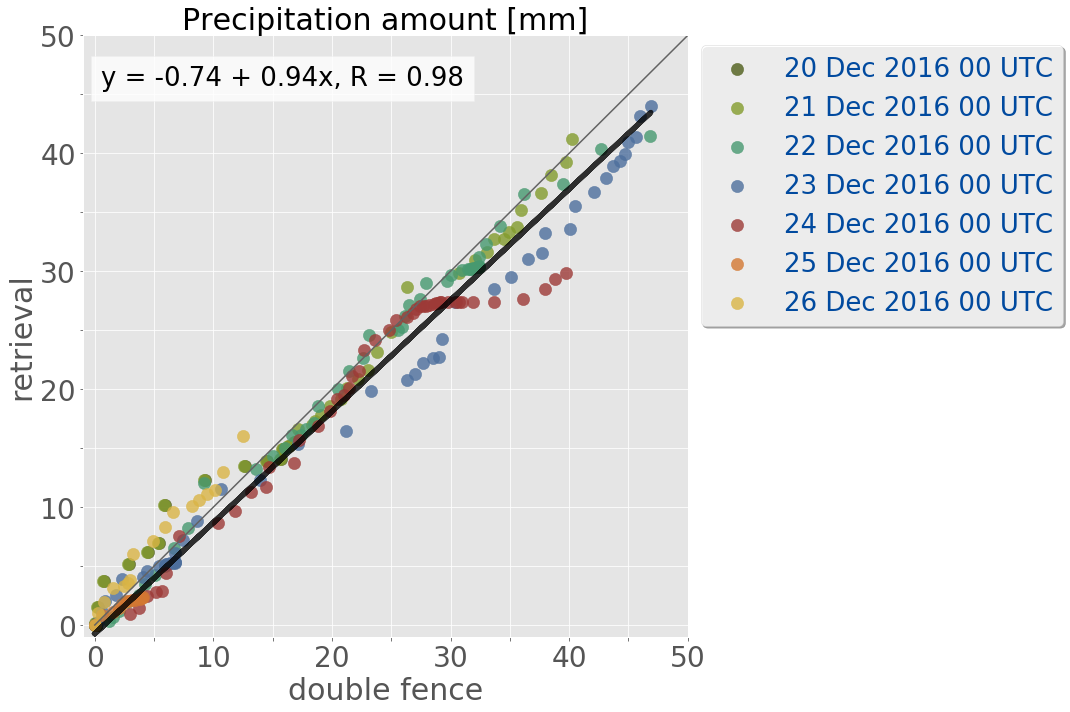
\includegraphics[trim={0.cm 0.cm 13cm 0cm},clip,
    width=\textwidth]{./fig_obs_ret/obs_ret_20161220_26_00}
    \caption{}\label{fig:res:obs_ret_scatter}
    \end{subfigure}
    %
    \begin{subfigure}[b]{0.59\textwidth}
    	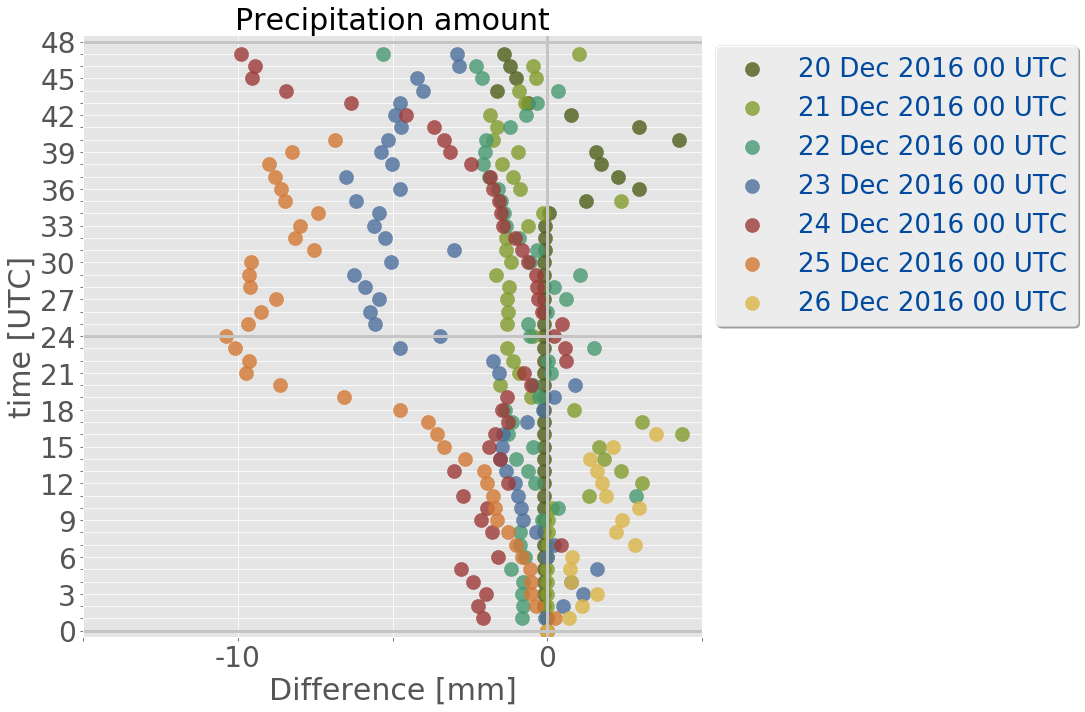
\includegraphics[trim={0.cm 0.cm 0cm 0cm},clip,
    width=\textwidth]{./fig_obs_ret/diff_20161220_26_00}
    \caption{}\label{fig:res:diff_ret_scatter}
    \end{subfigure}
    % label
%    \begin{subfigure}[t]{0.18\textwidth}
 %   	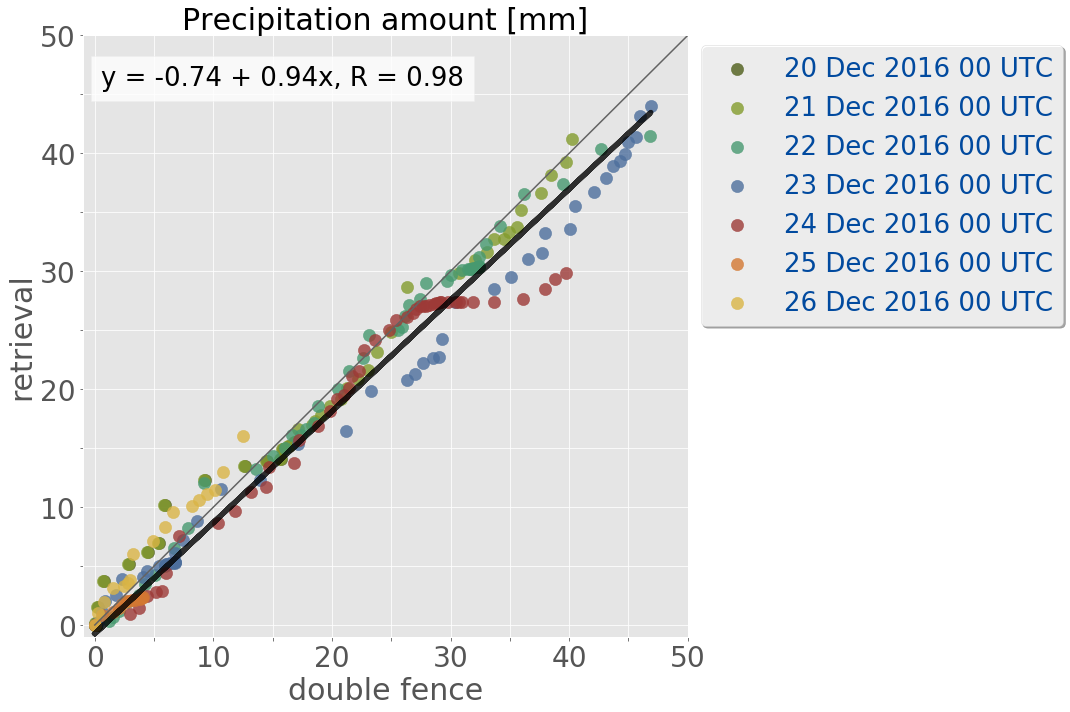
\includegraphics[trim={25.cm 13.cm 0cm 1.3cm},clip,
  %  width=\textwidth]{./fig_obs_ret/obs_ret_20161220_26_00}
   % \end{subfigure}
    
    \caption{Scatter plot comparing the observed and retrieved \SI{48}{\hour} surface accumulation (\protect\subref{fig:res:obs_ret_scatter}).  In black the linear regression between the two systems. \protect\subref{fig:res:diff_ret_scatter}: Difference between the retrieved surface accumulation and the observed accumulation by the double fence. The colours represent the days of the storm with the start of calculated \SI{48}{\hour} accumulation at \SI{0}{\UTC}. Accumulations starting on the \SI{25}{\dec} are not a fair comparison because of observed liquid precipitation. }\label{fig:res:obs_ret}
\end{figure}
%%%%%%%%%%%%%%%%%%%%%%%%%%%%%%%%%%%%%%%%%%%%%%
To be able to compare an analysis of the vertical predicted snow water content and the observed snow water content an a verification of the surface accumulation must be made. If the retrieved surface accumulation is confident in comparison to the double fence measurement then the vertical can be trusted.
\\
Comparison of the \SI{48}{\hour} accumulation demonstrate a good agreement between double fence observations and retrieved surface accumulation. \Cref{fig:res:obs_ret_scatter} shows the agreement between the two systems. The black line in \Cref{fig:res:obs_ret_scatter} presents a linear correlation with a coefficient of R = \num{0.97}. 
\\
In general underestimates the surface snowfall accumulation. \Cref{fig:res:diff_ret_scatter} shows the difference between retrieved accumulation and observed accumulation by the double fence. For \SIrange{20}{24}{\dec} \Cref{fig:res:diff_ret_scatter} indicates an underestimation of less than \SI{-5}{\mm} for the first \SI{24}{\hour}. After \SI{24}{\hour} shows especially the \SI{23}{\dec} an underestimation of up to \SI{-6.5}{\mm} and \SI{24}{\dec} underestimates larger than \SI{-6.3}{\mm} after \SI{43}{\hour}. The mean absolute error of all days is $\pm$\SI{2.06}{\mm} (excluding values on \SI{25}{\dec} after \SI{12}{\UTC} because of liquid precipitation and on \SI{26}{\dec} after \SI{17}{\UTC} because of attenuation at the MRR). The error is only representative for the Christmas storm, more storms should be investigated to find the absolute correlation between surface observation and estimated accumulation by using vertical data.
Since the bias is not large between double fence observations and retrieved surface accumulation can the vertical retrieved snow water content be trusted. 

%%%%%%%%%%%%%%%%%%%%%%%%%%%%%%%%%%%%%%%%%%%%%%%%%%%%%%%%%%%%%%%%%%%%%%%%%%

%%%%%%%%%%%%%%%%%%%%%%%%%%%%%%%%%%%%%%%%%%%%%%%%%%%%%%%%%%%%%%%%%%%%%%%%%%
%%%%%%%%% Synoptic Phenomena observed? %%%%%%%%%%%%%%
\section{Observation of large scale weather phenomena at the surface}
%%%%%%% image scatter obs ret %%%%%%%%%%%%%%%%
\begin{figure}[h!]
	\centering
    % sfc pressure
    \begin{subfigure}[b]{0.49\textwidth}
    	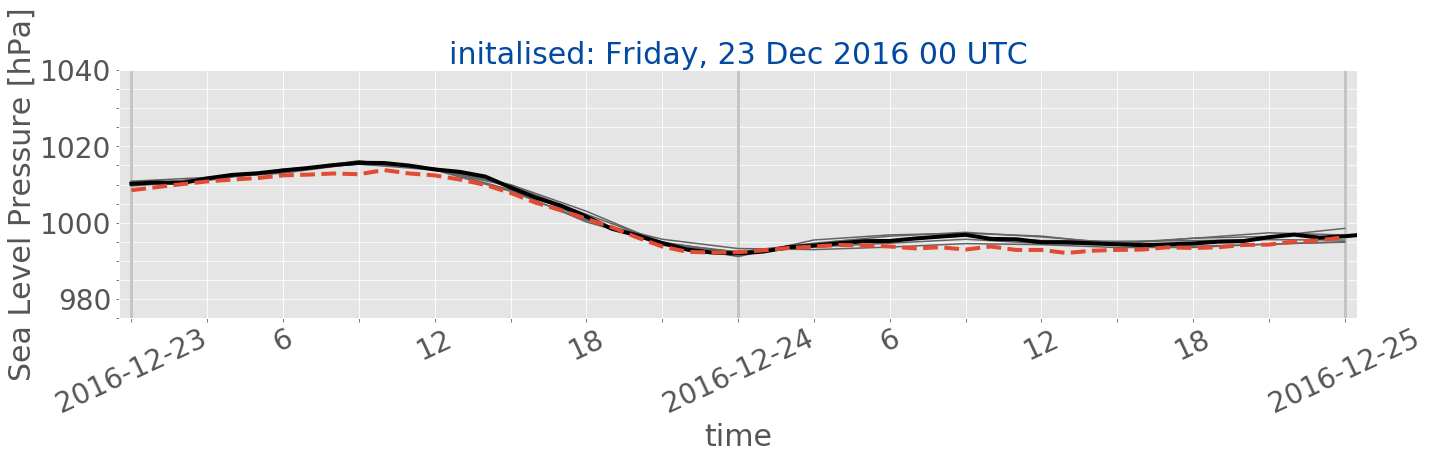
\includegraphics[trim={0.cm 3.6cm 0cm 0cm},clip,
    width=\textwidth]{./fig_sfc_pressure/20161223_00}
    	\caption{}\label{fig:res:sfc_pres23}
    \end{subfigure}
    %
    \begin{subfigure}[b]{0.49\textwidth}
    	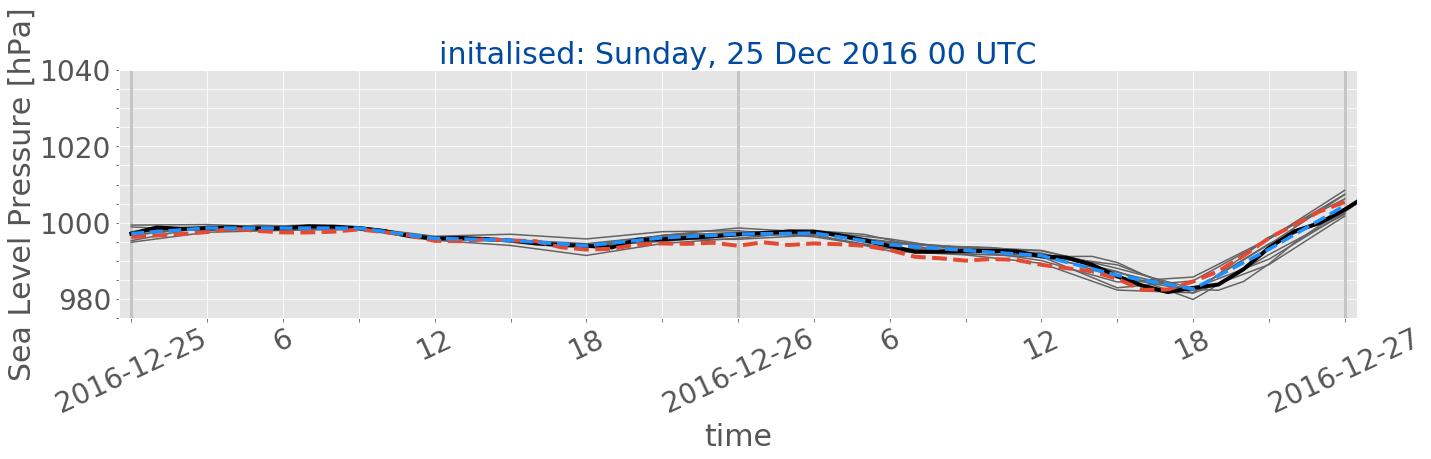
\includegraphics[trim={0.cm 3.6cm 0cm 0cm},clip,
    width=\textwidth]{./fig_sfc_pressure/20161225_00}
    	\caption{}\label{fig:res:sfc_pres25}
    \end{subfigure}
    % sfc temp
    \begin{subfigure}[b]{0.49\textwidth}
    	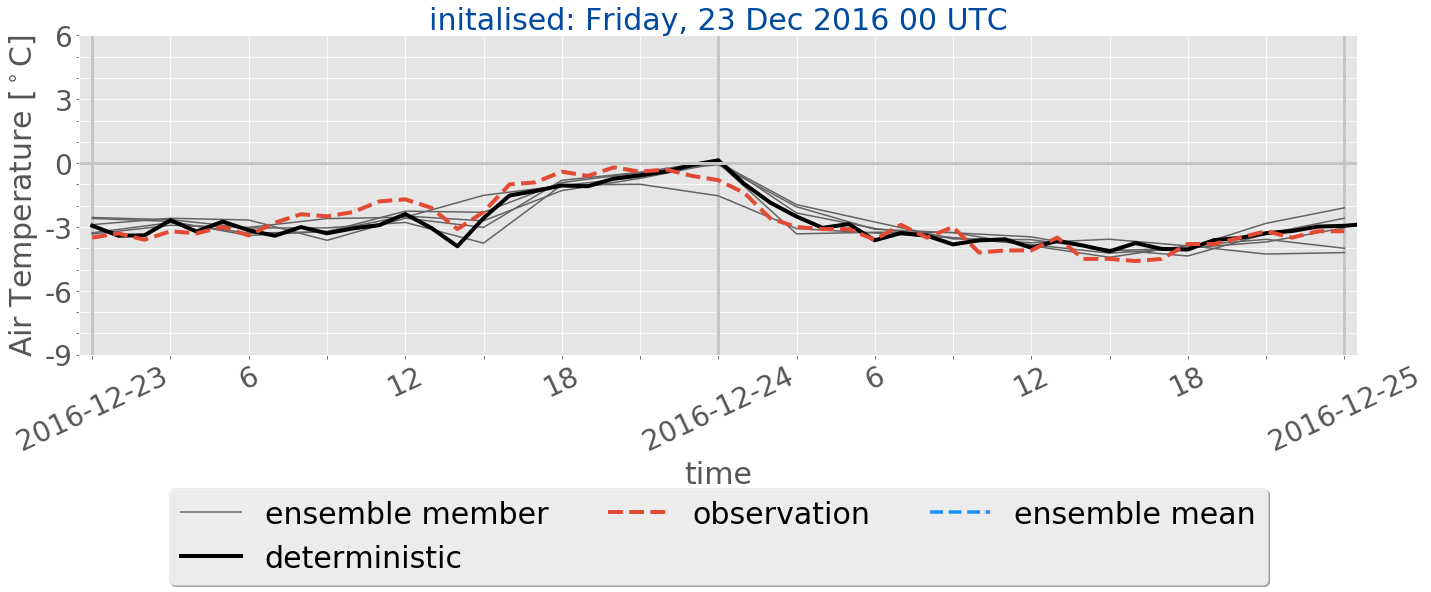
\includegraphics[trim={0.cm 3.6cm 0cm 0cm},clip,
    width=\textwidth]{./fig_sfc_temp/20161223_00}
    	\caption{}\label{fig:res:sfc_temp23}
    \end{subfigure}
    %
    \begin{subfigure}[b]{0.49\textwidth}
    	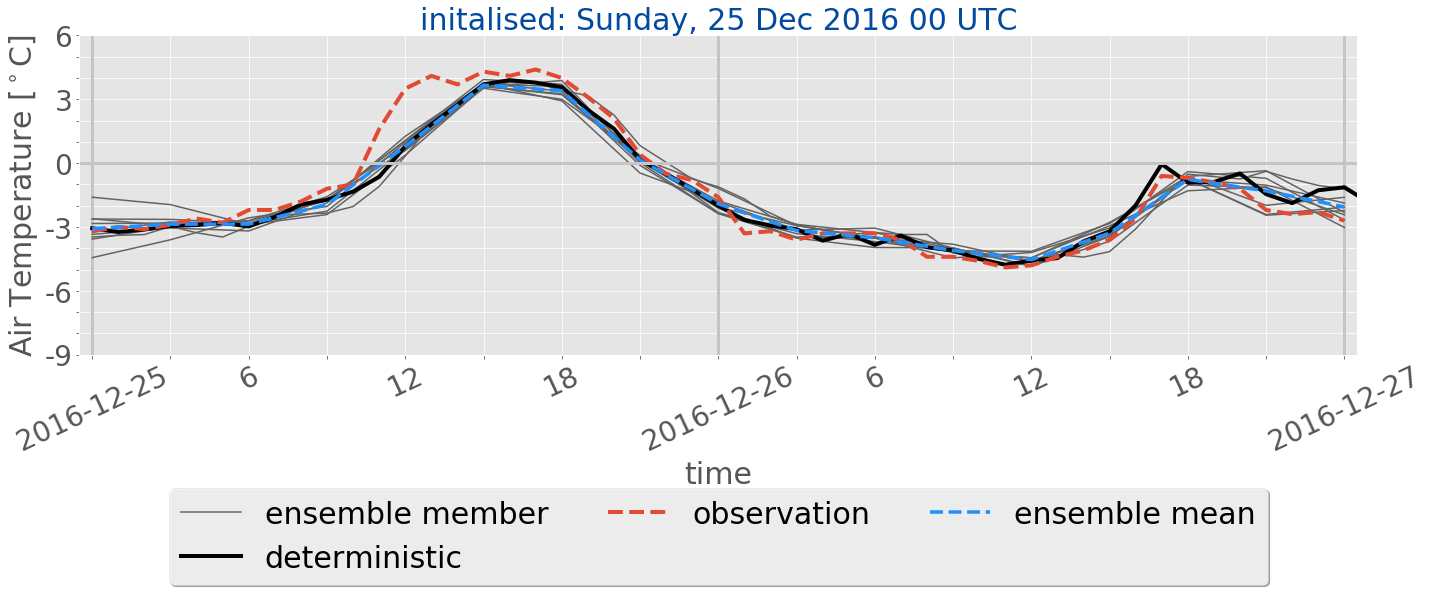
\includegraphics[trim={0.cm 3.6cm 0cm 0cm},clip,
    width=\textwidth]{./fig_sfc_temp/20161225_00}
    	\caption{}\label{fig:res:sfc_temp25}
    \end{subfigure}
    % sfc wd
    \begin{subfigure}[b]{0.49\textwidth}
    	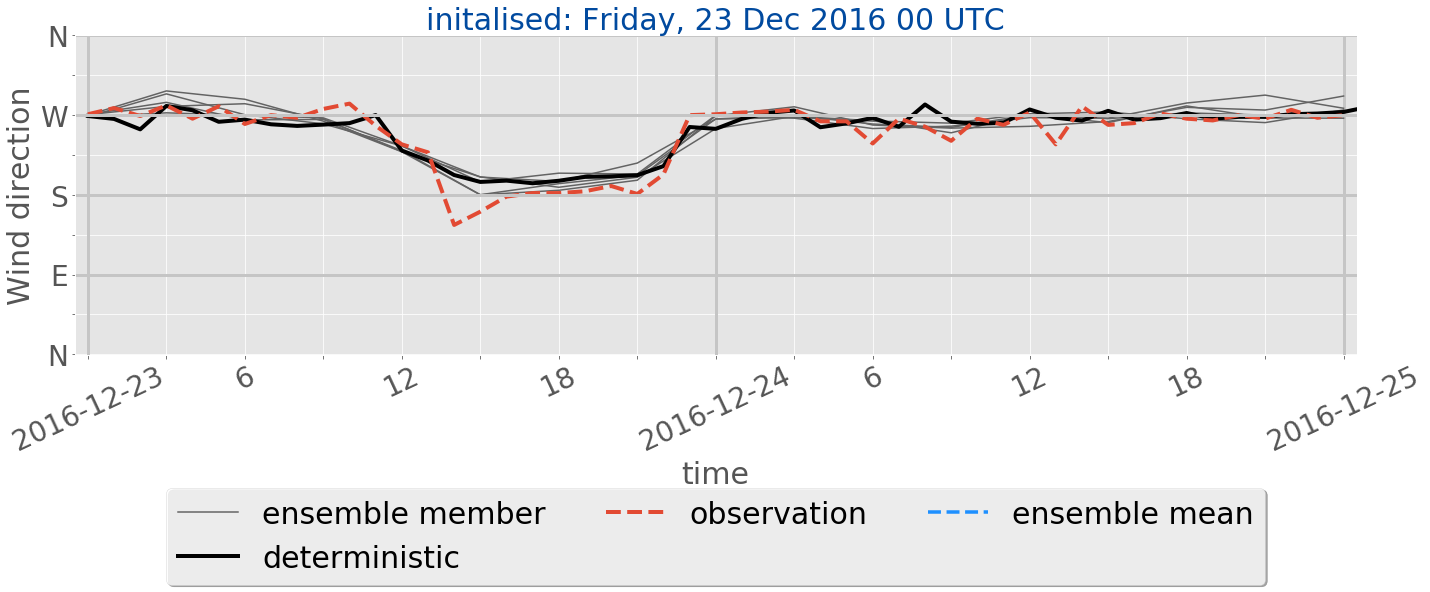
\includegraphics[trim={0.cm 3.6cm 0cm 0cm},clip,
    width=\textwidth]{./fig_sfc_wd/20161223_00}
    	\caption{}\label{fig:res:sfc_wd23}
    \end{subfigure}
    %
    \begin{subfigure}[b]{0.49\textwidth}
    	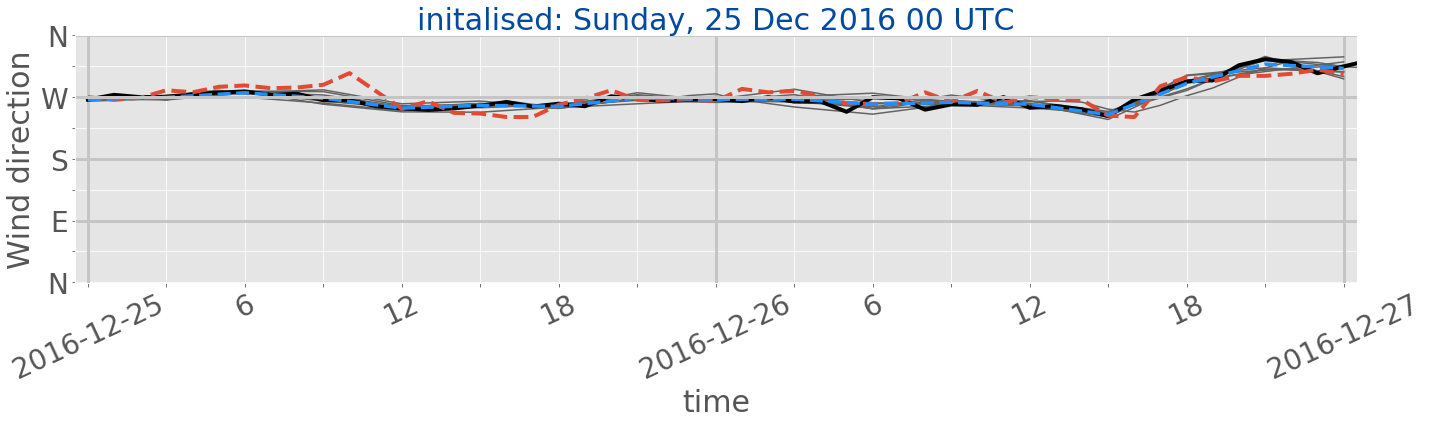
\includegraphics[trim={0.cm 3.6cm 0cm 0cm},clip,
    width=\textwidth]{./fig_sfc_wd/20161225_00}
    	\caption{}\label{fig:res:sfc_wd25}
    \end{subfigure}
    % sfc ws
    \begin{subfigure}[b]{0.49\textwidth}
    	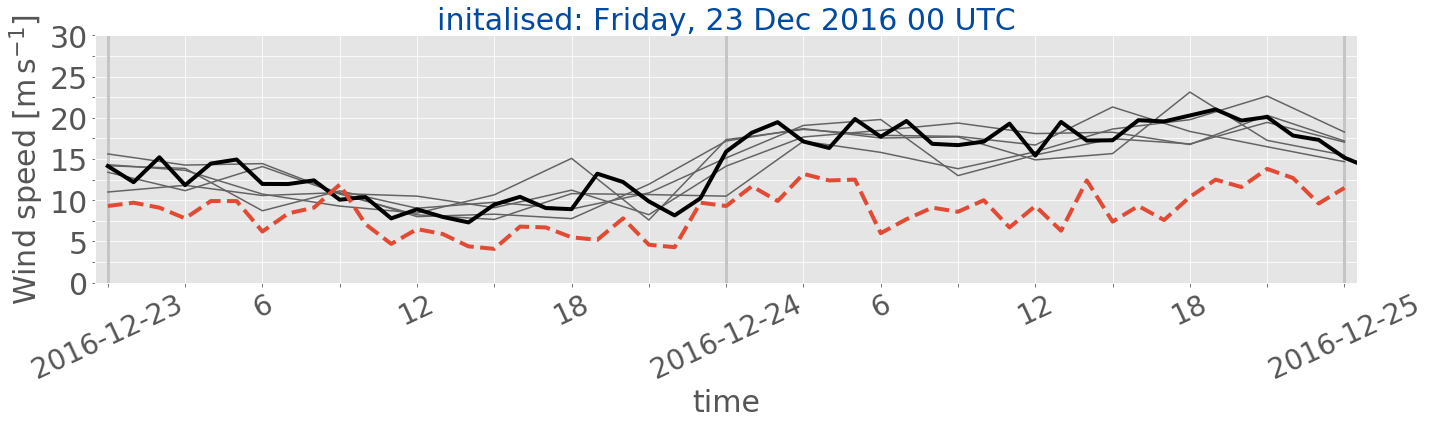
\includegraphics[trim={0.cm 3.6cm 0cm 0cm},clip,
    width=\textwidth]{./fig_sfc_ws/20161223_00}
    	\caption{}\label{fig:res:sfc_ws23}
    \end{subfigure}
    %
    \begin{subfigure}[b]{0.49\textwidth}
    	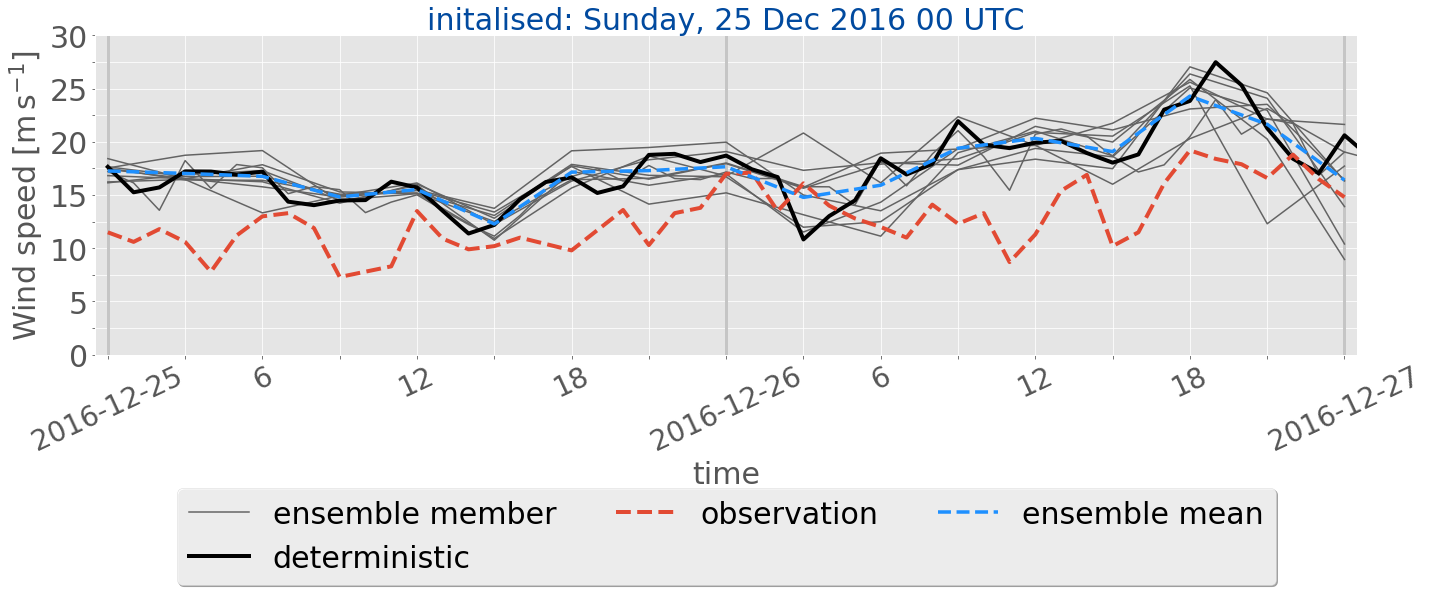
\includegraphics[trim={0.cm 3.6cm 0cm 0cm},clip,
    width=\textwidth]{./fig_sfc_ws/20161225_00}
    	\caption{}\label{fig:res:sfc_ws25}
    \end{subfigure}
    % sfc precip
    \begin{subfigure}[b]{0.49\textwidth}
    	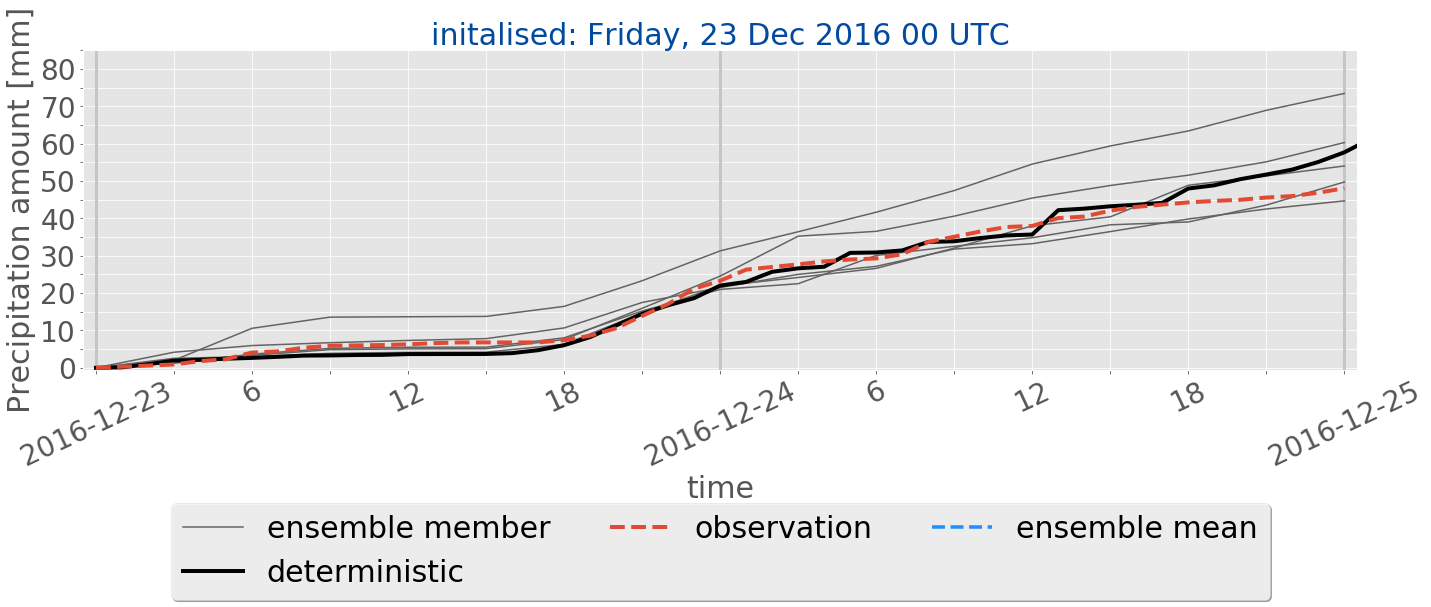
\includegraphics[trim={0.cm 3.6cm 0cm 0cm},clip,
    width=\textwidth]{./fig_sfc_precip/20161223_00}
    	\caption{}\label{fig:res:sfc_precip23}
    \end{subfigure}
    %
    \begin{subfigure}[b]{0.49\textwidth}
    	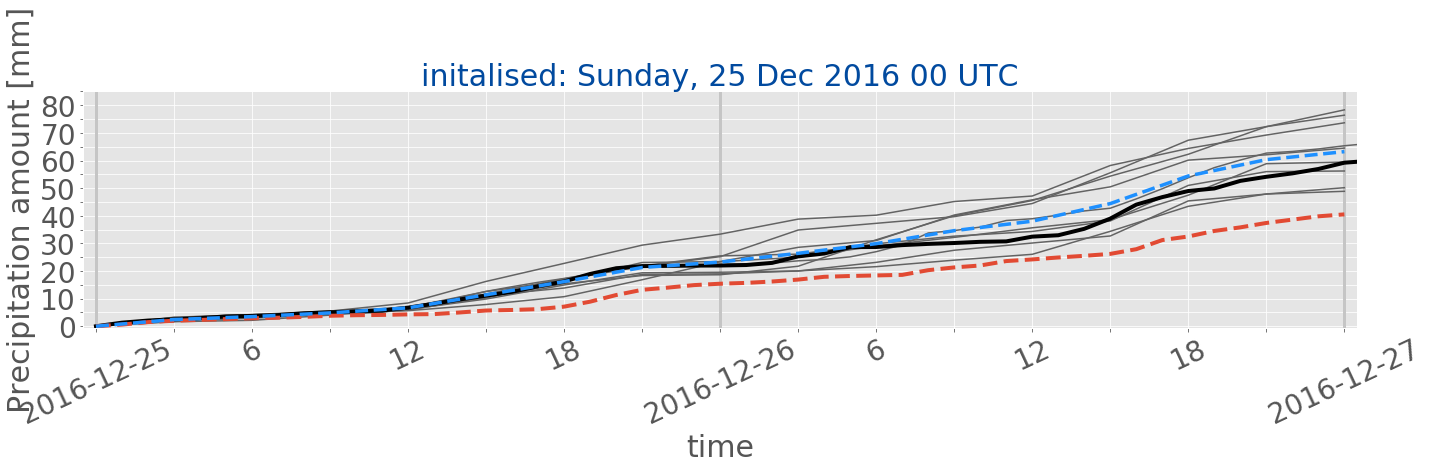
\includegraphics[trim={0.cm 3.6cm 0cm 0cm},clip,
    width=\textwidth]{./fig_sfc_precip/20161225_00}
    	\caption{}\label{fig:res:sfc_precip25}
    \end{subfigure}
    
    % label
    \begin{subfigure}[b]{\textwidth}
    \centering
 		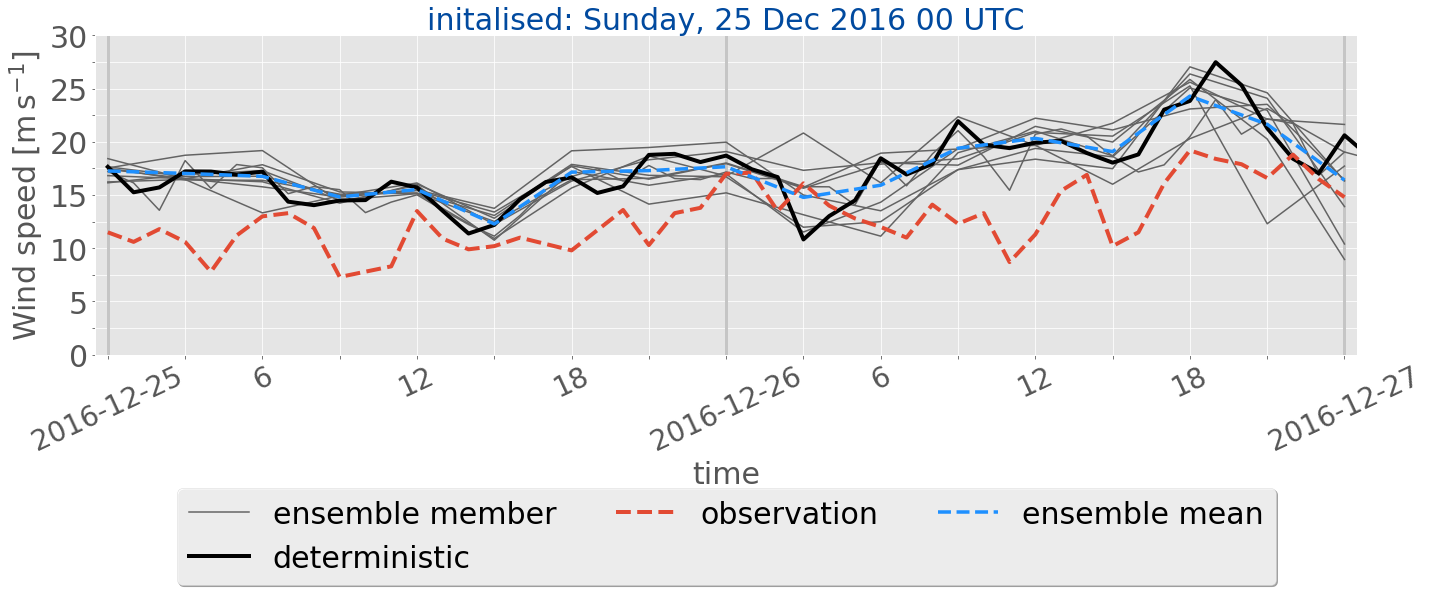
\includegraphics[trim={5.5cm 0cm 5.cm 17.2cm},clip,
    width=0.6\textwidth]{./fig_sfc_ws/20161225_00}
    \end{subfigure}
    %
\end{figure}
\begin{figure}\ContinuedFloat
	\centering
    % sfc pressure
    \begin{subfigure}[b]{0.49\textwidth}
		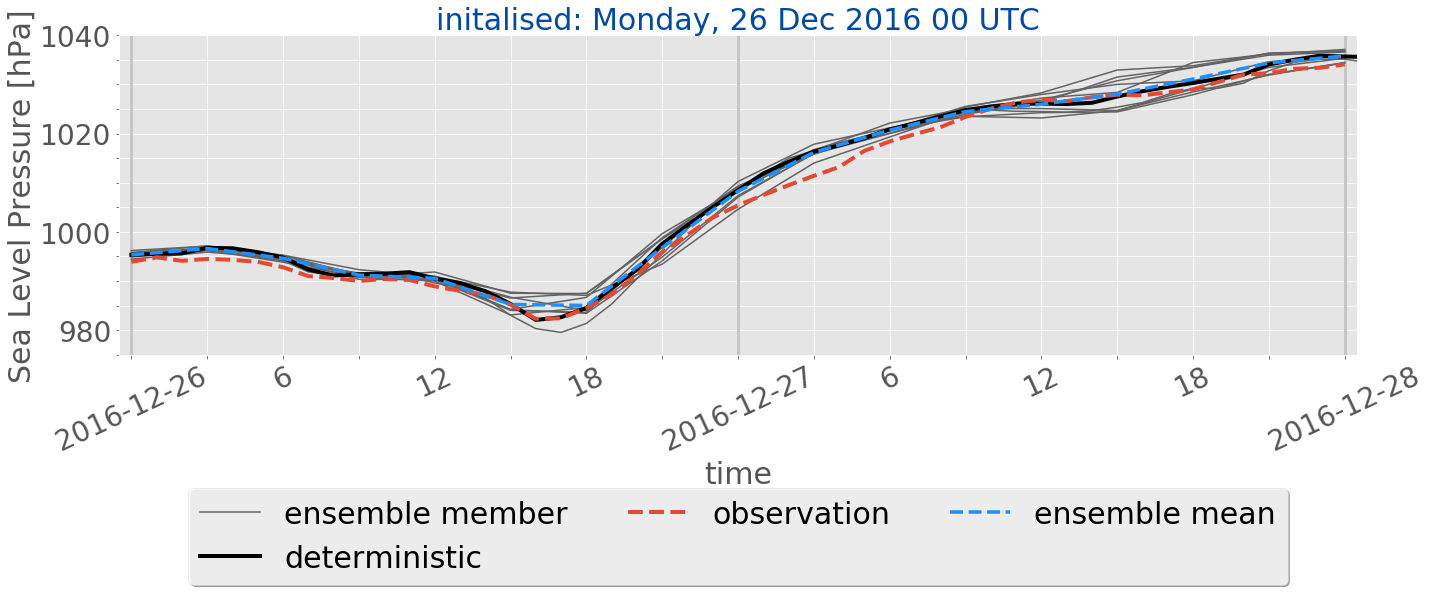
\includegraphics[trim={0.cm 3.6cm 0cm 0cm},clip,
    width=\textwidth]{./fig_sfc_pressure/20161226_00}
    	\caption{}\label{fig:res:sfc_pres26}
	\end{subfigure}
    
    % sfc temp
    \begin{subfigure}[b]{0.49\textwidth}
    	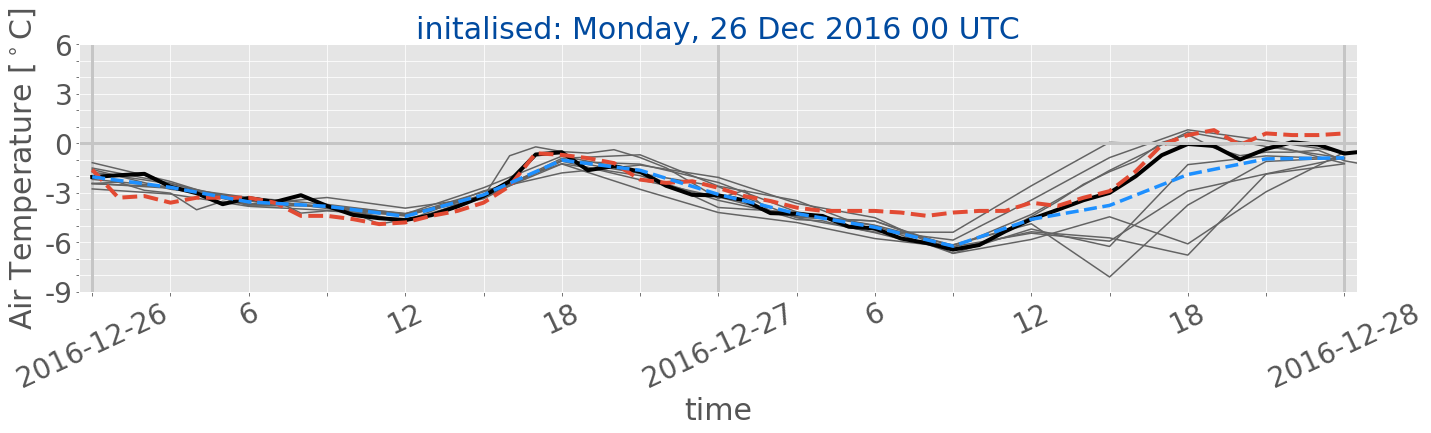
\includegraphics[trim={0.cm 3.6cm 0cm 0cm},clip,
    width=\textwidth]{./fig_sfc_temp/20161226_00}
    	\caption{}\label{fig:res:sfc_temp26}
    \end{subfigure}
    
    % sfc wd
    \begin{subfigure}[b]{0.49\textwidth}
    	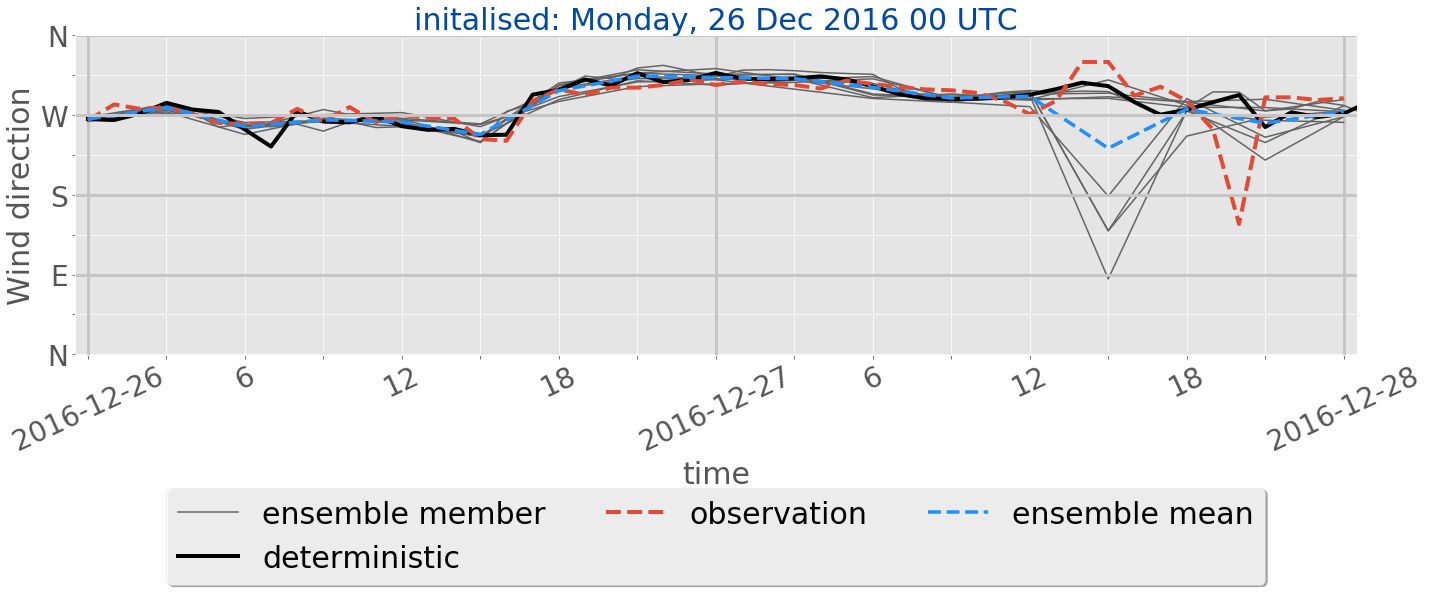
\includegraphics[trim={0.cm 3.6cm 0cm 0cm},clip,
    width=\textwidth]{./fig_sfc_wd/20161226_00}
    	\caption{}\label{fig:res:sfc_wd26}
    \end{subfigure}
    
    % sfc ws
    \begin{subfigure}[b]{0.49\textwidth}
    	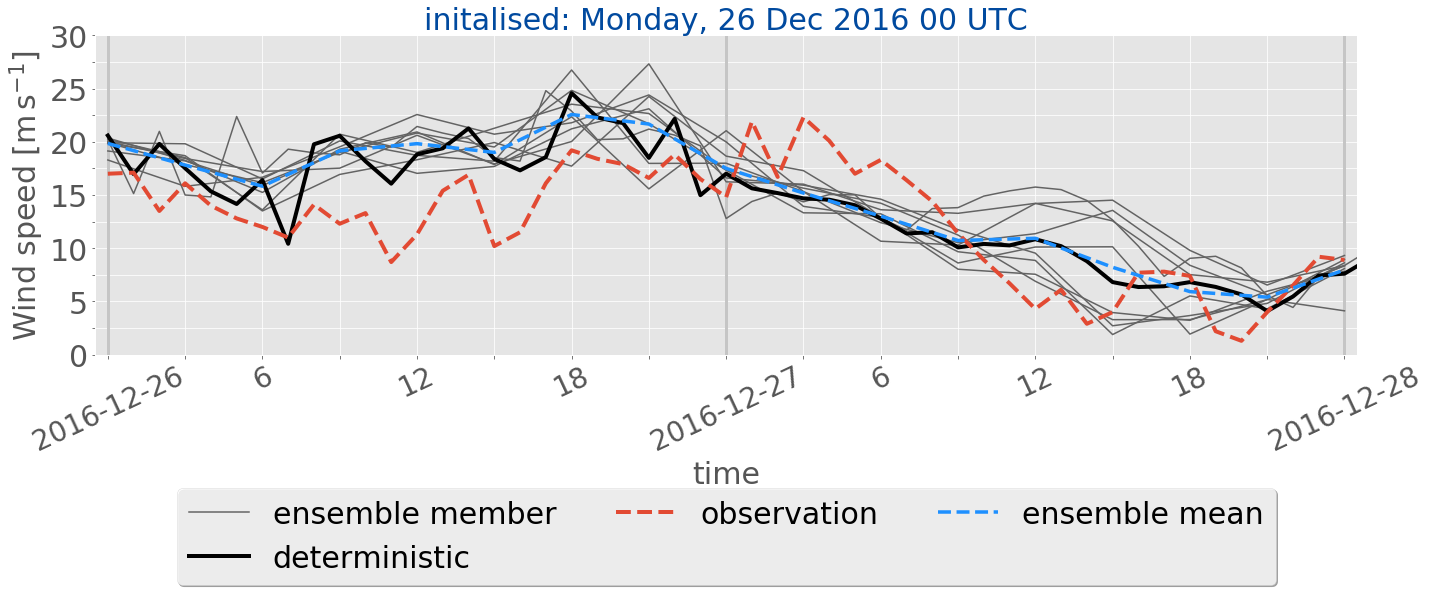
\includegraphics[trim={0.cm 3.6cm 0cm 0cm},clip,
    width=\textwidth]{./fig_sfc_ws/20161226_00}
    	\caption{}\label{fig:res:sfc_ws26}
    \end{subfigure}
    
    % sfc precip
    \begin{subfigure}[b]{0.49\textwidth}
    	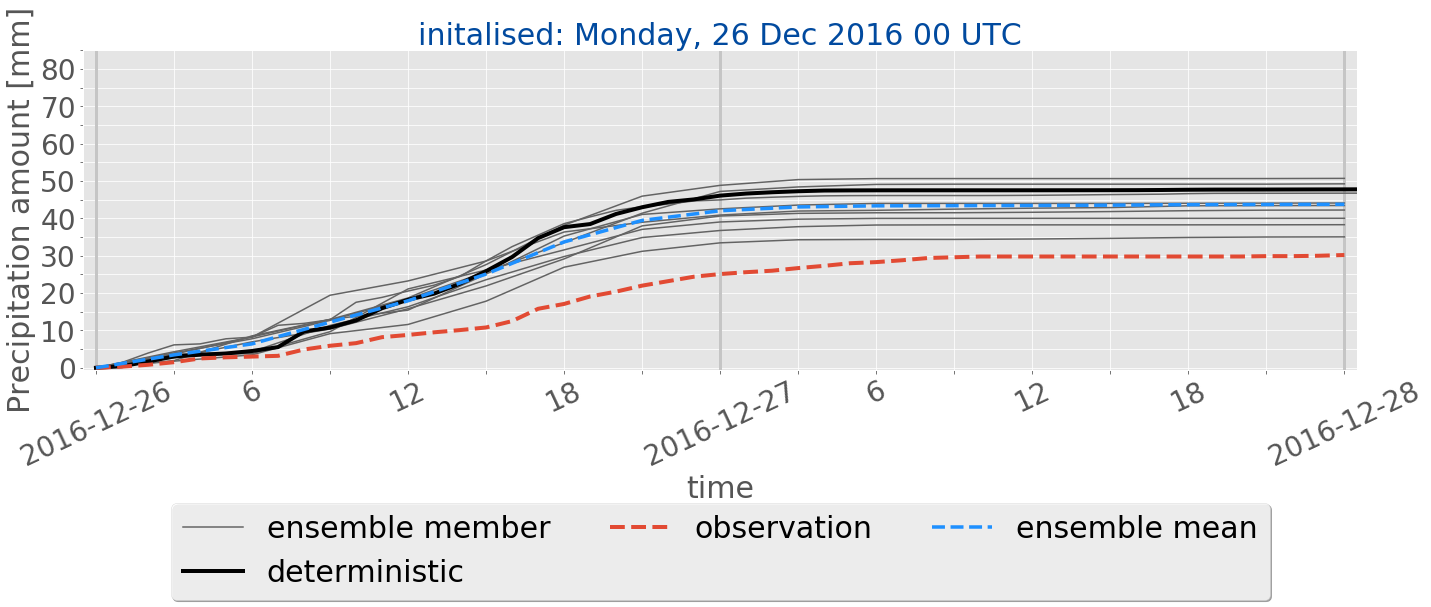
\includegraphics[trim={0.cm 3.6cm 0cm 0cm},clip,
    width=\textwidth]{./fig_sfc_precip/20161226_00}
    	\caption{}\label{fig:res:sfc_precip26}
    \end{subfigure}
    
    % label
    \begin{subfigure}[b]{\textwidth}
    	\centering
 		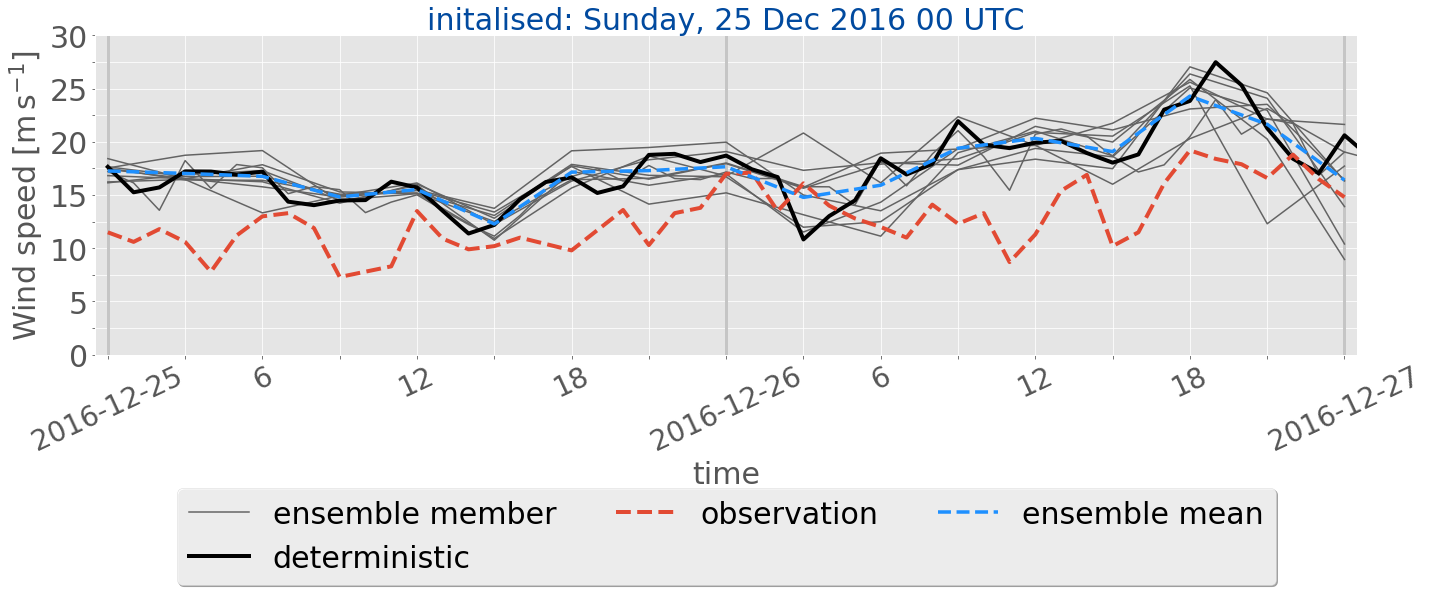
\includegraphics[trim={5.5cm 0cm 5.cm 17.2cm},clip,
    width=0.6\textwidth]{./fig_sfc_ws/20161225_00}
    \end{subfigure}
    \caption{\SI{48}{\hour} surface observations and ensemble forecasts initialised on the \SI{23}{\dec} (left column, previous page, \protect\subref{fig:res:sfc_pres23}, \protect\subref{fig:res:sfc_temp23}, \protect\subref{fig:res:sfc_wd23}, \protect\subref{fig:res:sfc_ws23}, \protect\subref{fig:res:sfc_precip23}), and on \SI{25}{\dec} (right column, previous page, \protect\subref{fig:res:sfc_pres25}, \protect\subref{fig:res:sfc_temp25}, \protect\subref{fig:res:sfc_wd25}, \protect\subref{fig:res:sfc_ws25}, \protect\subref{fig:res:sfc_precip25}) as well as \SI{25}{\dec} (\protect\subref{fig:res:sfc_pres26}, \protect\subref{fig:res:sfc_temp26}, \protect\subref{fig:res:sfc_wd26}, \protect\subref{fig:res:sfc_ws26}, \protect\subref{fig:res:sfc_precip26}). Line representation according to the label. Upper panel sea level pressure, second \SI{2}{\metre} air temperature, third and forth \SI{10}{\metre} wind direction and speed, respectively, and lowest panel precipitation amount. }\label{fig:res:sfc_obs_meps}
\end{figure}
%%%%%%%%%%%%%%%%%%%%%%%%%%%%%%%%%%%%%%%%%%%%%%
One of the main factors, that made this particular case so interesting is the fact, that several times in the six day period frontal boundaries passed over Norway. The aim of this work is to determine if large scale features were observed at the measurement site. 
\\
When comparing the MEPS forecast of surface weather maps and the ECMWF analysis of dynamic tropopause maps, it shows that frontal passages occurred on three days during the Christmas storm (\Cref{fig:GeopJet} and \ref{fig:DynTropo}).  These frontal boundaries show in the surface observations and ensemble forecasts on \SIlist{23;25;26}{\dec}. A typical cyclone has a prevailing warm front and a faster moving cold front. As the storm gets more intense and the cold front rotates around the low pressure centre and catches the warm front. This follows an occluded front. Changes in pressures, temperature, wind direction and wind speed can occur. In some cases an intensification of the precipitation can be observed as well.
\\
\Cref{fig:res:sfc_obs_meps} shows the different parameters forecasts initialised at \SI{00}{\UTC} for \SIlist{23;25;26}{\dec}, as well as the observations at the Haukeliseter measurement site in dash-red.
Typical pressure decreases and increases, as well as temperature increases and wind changes are present on \SIlist{23;26}{\dec}. The \SI{25}{\dec} shows only a passage of a warm air mass. 
\\
As described in \Cref{sec:largeScale} shows the ECMWF dynamic tropopause analysis map (\Cref{fig:DT23}) more ridging and therefore warmer air over Southern Norway on \SI{23}{\dec}. The low pressure system approaches in the course of the day south-east Iceland and hence stronger west to south west wind are associated with the cyclone (\Cref{fig:GP23}). The MEPS forecast, initialised on \SI{23}{\dec} \SI{0}{\UTC} in \Cref{fig:res:sfc_pres23} shows the decrease in pressure after \SI{12}{\UTC} due to the passage of the occluded front with a constant pressure after the transition. Since warmer air is more advected to the North and the DT in \Cref{fig:DT23} shows a warmer low pressure core, an increase in temperature was observed and predicted at the measurement site (\Cref{fig:res:sfc_temp23}). 
\\
As the cyclone is advected to the north-east, closer into the Norwegian Sea, a wind change can be seen in the analysis map from ECMWF (\Cref{fig:GP23}, were first west wind and later south-west wind was associated with the low pressure system. In \Cref{fig:res:sfc_wd23} and \subref{fig:res:sfc_ws23} a similar wind change can be observed by the MEPS forecast and observations.
\\
On \SI{23}{\dec} was the passage of the occlusion also observed by an increase in precipitation. Before \SI{18}{\UTC} shows the surface accumulation light precipitation. During the passage of the occluded front increases the observed surface accumulation and is associated to continuous, heavy precipitation.
\\
\\
Similar patterns were seen for the passage of the occluded front on \SI{26}{\dec} in the ECMWF analysis \Cref{fig:DT26} and \ref{fig:GP26}. In this case the low pressure system was located north of Morø og Romsdal in the Norwegian Sea. In the morning was the low cyclone located east of Iceland and in the course of the day it got closer to the coast of Norway. Before landfall at \SI{16}{\UTC} demonstrates \Cref{fig:res:sfc_pres26} a pressure decrease. During the passage the sea level pressure decreases its lowest point of \SI{985}{\hPa}, and increased afterwards during the dissipation of the Christmas storm.
\\
Since the cyclone was surrounded by colder air (south of the low pressure system) first a drop and then an increase of temperature were observed and forecasted by MEPS. An indication of the passage is also seen in the \SI{10}{\metre} wind observations and forecasts. As the cyclone is east of Iceland with a westward large scale surface wind (\Cref{fig:GP26_00} and \Cref{fig:GP26_12}), shows \Cref{fig:res:sfc_wd26} west wind wind with observed strength up to \SI{17.5}{\mPs} (\Cref{fig:res:sfc_ws26}). During the passage changes the wind direction to north-west with higher wind speed which can be associated to the location of the low pressure system and the closer surface isobars (\Cref{fig:DT26}). 
\\
The precipitation was continues throughout the day, with light to moderate precipitation before the passage and heavy precipitation around \SI{16}{\UTC} followed by moderate to light.
\\
\\
While on \SIlist{23;25}{\dec} the precipiation was associated with a passage/landfall of an occluded front, was the \SI{25}{\dec} marked by the transition of a warm sector. The ECMWF analysis showed a ridging at the DT surface. The surface cyclone core is south east of Iceland in \Cref{fig:DT25} with two associated frontal boundaries. While the warm front is aproaching the west coast, is the cold front north west of Great Britain. The cold fronts tail moved into lower latitudes, following the slow down of the cold front, leading to a stationary frontal boundary. Further more the mid-latidual jet is aligned along the surface frontal boundaries (\Cref{fig:DT25_00}), while the Haukeliseter site is located below the left jet exit region. This leads to rising motion at the surface.
\\
Neither pressure nor wind observations and forecasts indicate the passage of any frontal boundary. The only indication of the transition is seen in the increase of temperature at \SI{11}{\UTC} until \SI{21}{\UTC} (\Cref{fig:res:sfc_temp25}). In \Cref{fig:res:sfc_wd25} a small wind change was observed from west to north-west by the wind mast at \SI{10}{\UTC}, but the forecast does not show this wind change for an initialisation on \SI{25}{\dec}. 
\\
%%%%%%% image liquid obs particle %%%%%%%%%%%%%%%%
\begin{figure}[t]
	\centering
	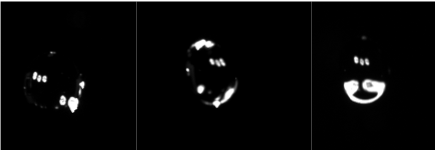
\includegraphics[%trim={45.cm 30.cm 13cm 35cm},clip,
    width=0.8\textwidth]{./MASC_obs/Masc_obs_liquid_2512}
    \caption{MASC images of falling water drops observed on \SI{25}{\dec} at \SI{17}{\UTC} from three different angles. Not all parts of the liquid sphere are equally illuminated.}\label{fig:res:obs_masc}
\end{figure}
%%%%%%%%%%%%%%%%%%%%%%%%%%%%%%%%%%%%%%%%%%%%%%
In \Cref{fig:res:obs_masc} are the surface observations from the MASC during the passage of the warm sector. Without the images taken at \SI{17}{\UTC} at the Haukeliseter site it would not be possible to verify that liquid precipitation occurred. Together with the increase in surface temperature in \Cref{fig:res:sfc_temp25} it is qualified that at least the warm sector of the low pressure system appeared at the measurement site.
\\
%%%%%%% image scatter obs ret %%%%%%%%%%%%%%%%
\begin{figure}[h!]
	\centering
    % sfc pressure
    \begin{subfigure}[b]{0.49\textwidth}
    	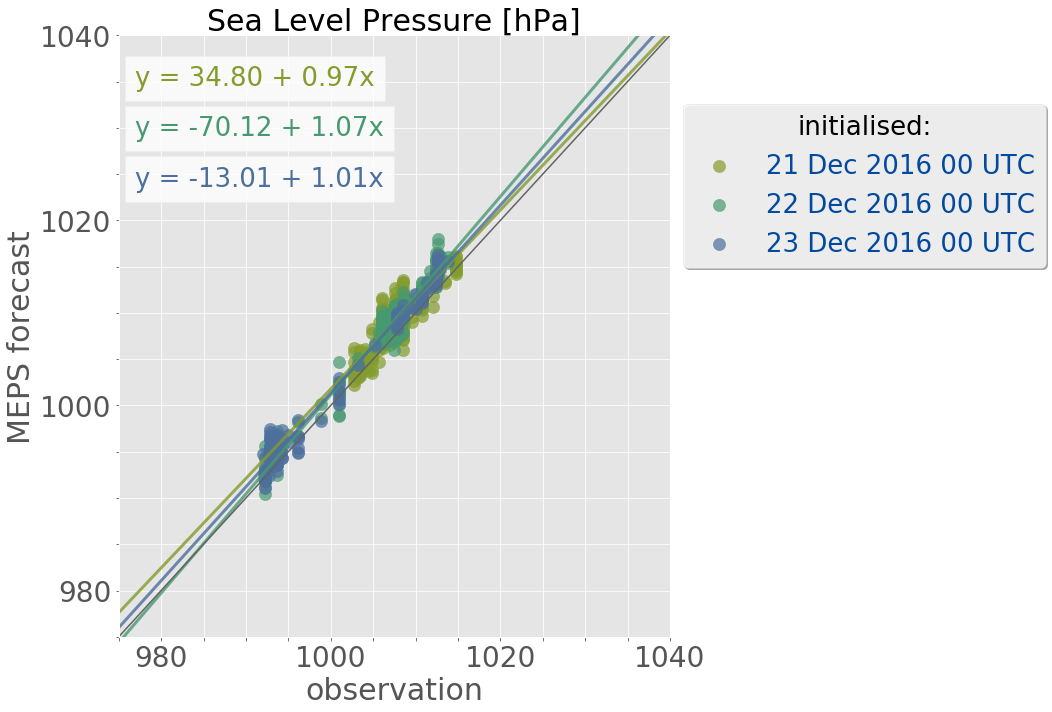
\includegraphics[trim={0.cm 0cm 12.5cm 0cm},clip,
    width=\textwidth]{./fig_sfc_pressure/obs_model_20161221_23_00}
    	\caption{}\label{fig:scat:pres2123}
    \end{subfigure}
    %
    \begin{subfigure}[b]{0.49\textwidth}
    	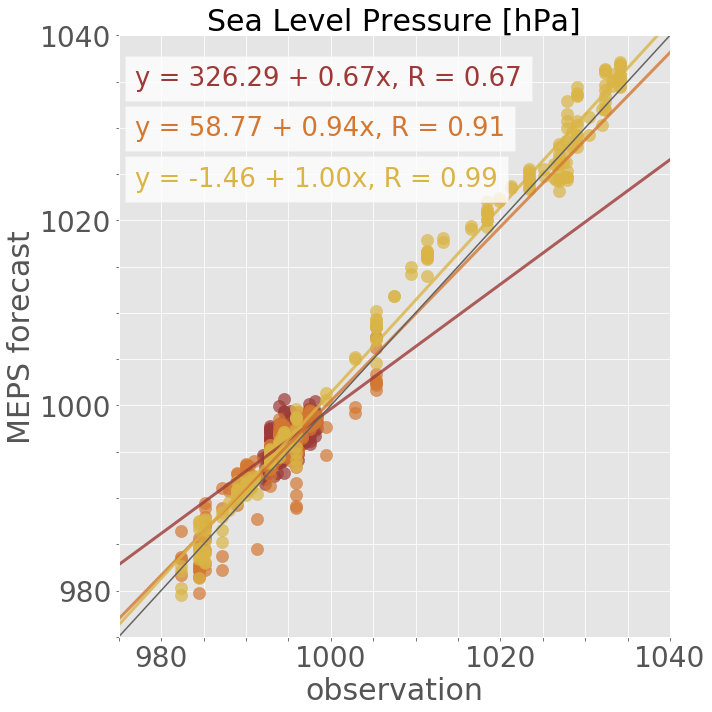
\includegraphics[trim={0.cm 0cm 12.5cm 0cm},clip,
    width=\textwidth]{./fig_sfc_pressure/obs_model_20161224_26_00}
    	\caption{}\label{fig:scat:pres2426}
    \end{subfigure}
%     % sfc temp
     \begin{subfigure}[b]{0.49\textwidth}
     	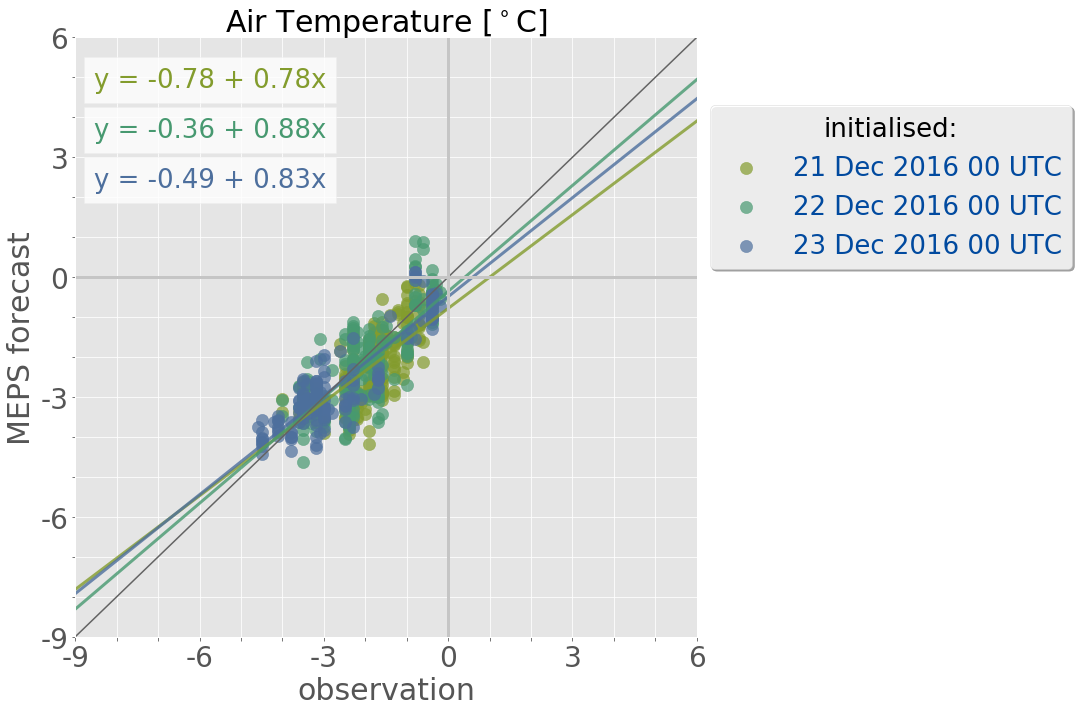
\includegraphics[trim={0.cm 0cm 12.5cm 0cm},clip,
    width=\textwidth]{./fig_sfc_temp/obs_model_20161221_23_00}
     	\caption{}\label{fig:scat:temp2123}
     \end{subfigure}
     %
	\begin{subfigure}[b]{0.49\textwidth}
     	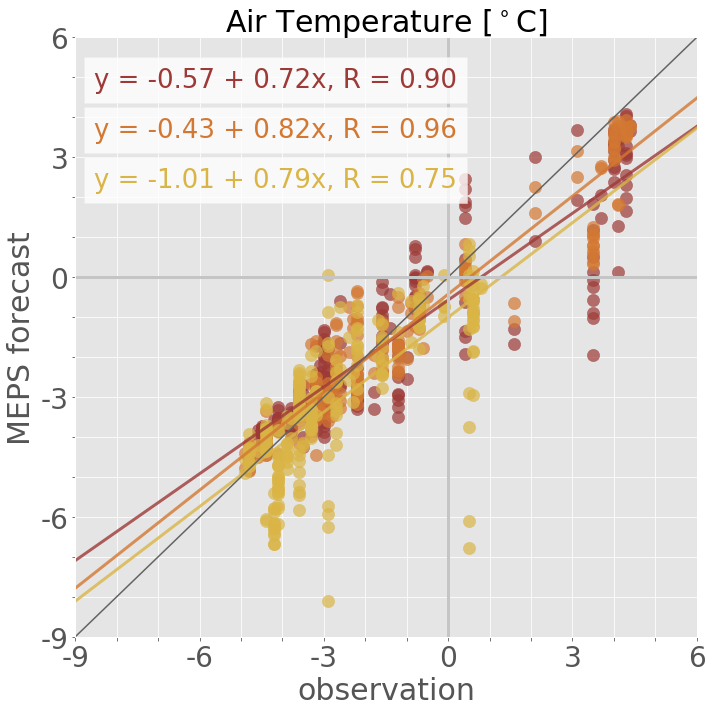
\includegraphics[trim={0.cm 0cm 12.5cm 0cm},clip,
    width=\textwidth]{./fig_sfc_temp/obs_model_20161224_26_00}
     	\caption{}\label{fig:scat:temp2426}
     \end{subfigure}
     
     % label
     \begin{subfigure}[b]{0.49\textwidth}
     	\centering
     	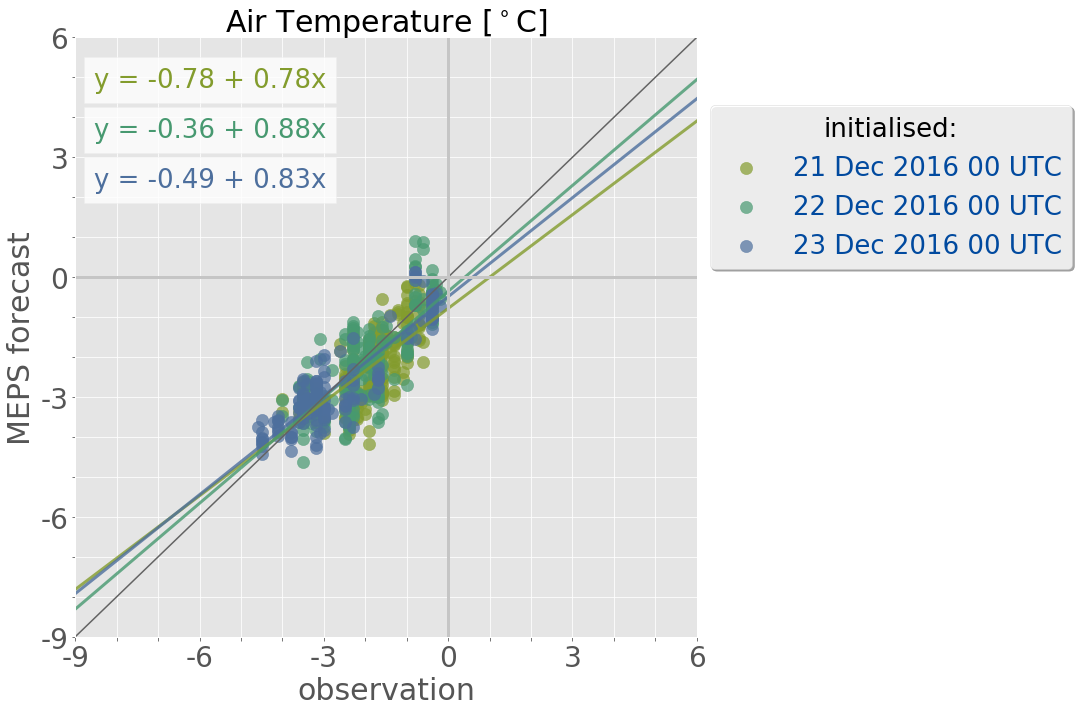
\includegraphics[trim={25.cm 15.5cm 0cm 3.6cm},clip,
    width=0.8\textwidth]{./fig_sfc_temp/obs_model_20161221_23_00}
     \end{subfigure}
     \begin{subfigure}[b]{0.49\textwidth}
     	\centering
     	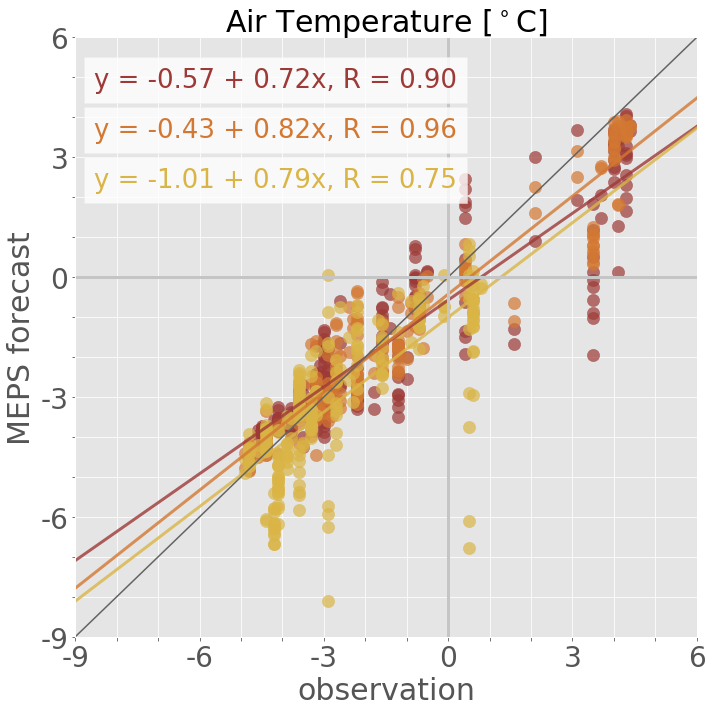
\includegraphics[trim={25.cm 15.5cm 0cm 3.6cm},clip,
    width=0.8\textwidth]{./fig_sfc_temp/obs_model_20161224_26_00}
     \end{subfigure}
\end{figure}
\begin{figure}\ContinuedFloat
     % sfc wd
	\begin{subfigure}[b]{0.49\textwidth}
     	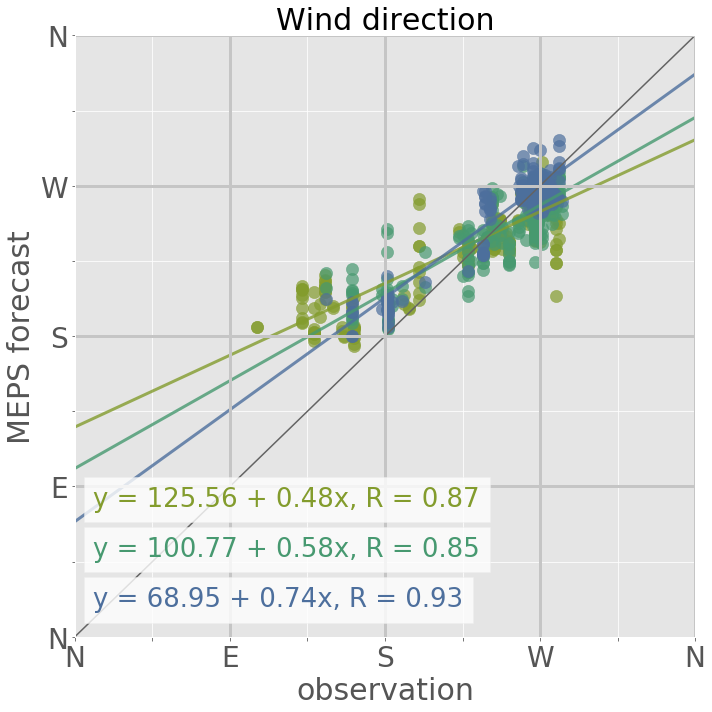
\includegraphics[trim={0.cm 0cm 12.5cm 0cm},clip,
    width=\textwidth]{./fig_sfc_wd/obs_model_20161221_23_00}
     	\caption{}\label{fig:scat:wd2123}
     \end{subfigure}
     %
	\begin{subfigure}[b]{0.49\textwidth}
     	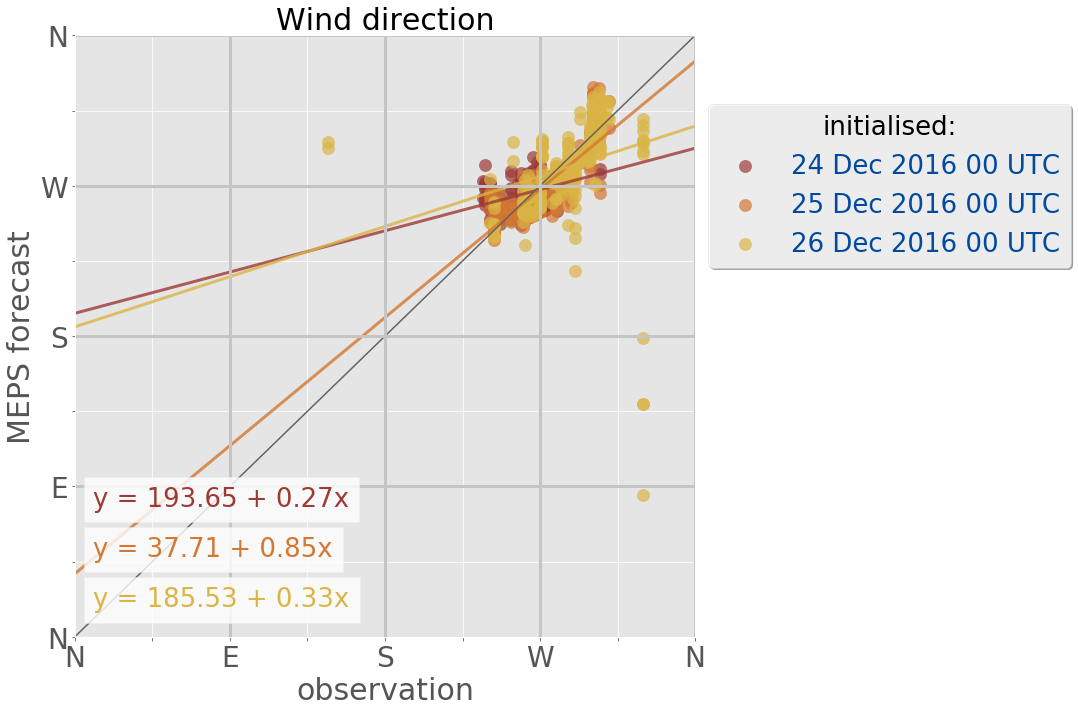
\includegraphics[trim={0.cm 0cm 12.5cm 0cm},clip,
    width=\textwidth]{./fig_sfc_wd/obs_model_20161224_26_00}
     	\caption{}\label{fig:scat:wd2426}
     \end{subfigure}
     % sfc ws
	\begin{subfigure}[b]{0.49\textwidth}
     	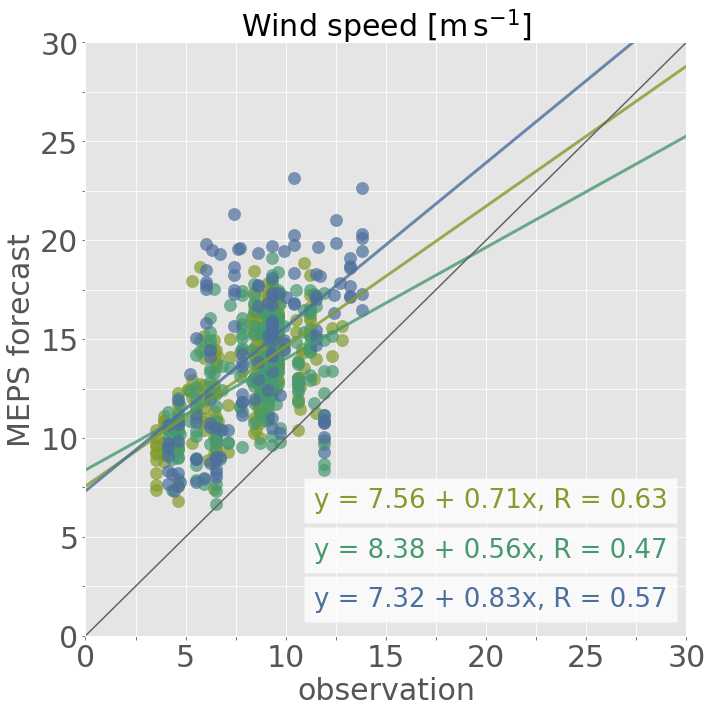
\includegraphics[trim={0.cm 0cm 12.5cm 0cm},clip,
    width=\textwidth]{./fig_sfc_ws/obs_model_20161221_23_00}
     	\caption{}\label{fig:scat:ws2123}
     \end{subfigure}
     %
	\begin{subfigure}[b]{0.49\textwidth}
     	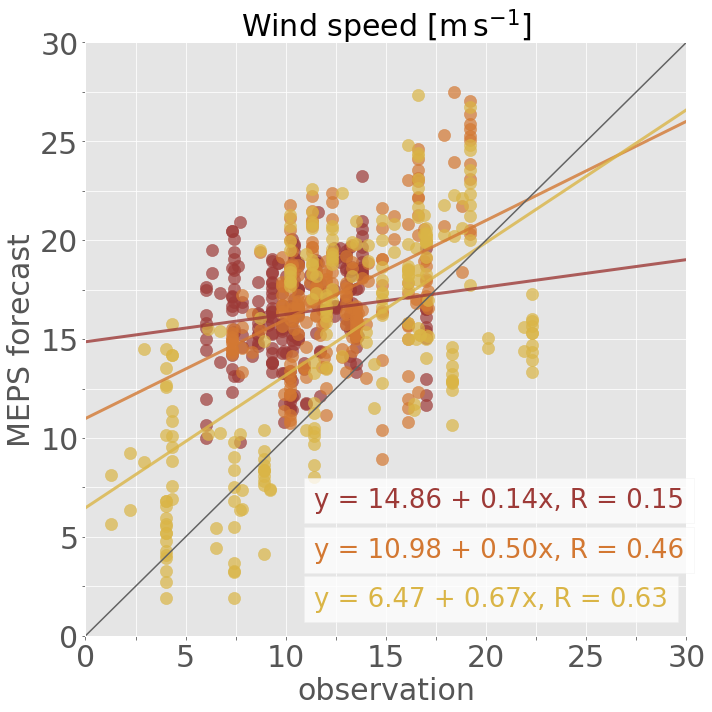
\includegraphics[trim={0.cm 0cm 12.5cm 0cm},clip,
    width=\textwidth]{./fig_sfc_ws/obs_model_20161224_26_00}
     	\caption{}\label{fig:scat:ws2426}
     \end{subfigure}
     % label
     \begin{subfigure}[b]{0.49\textwidth}
     	\centering
     	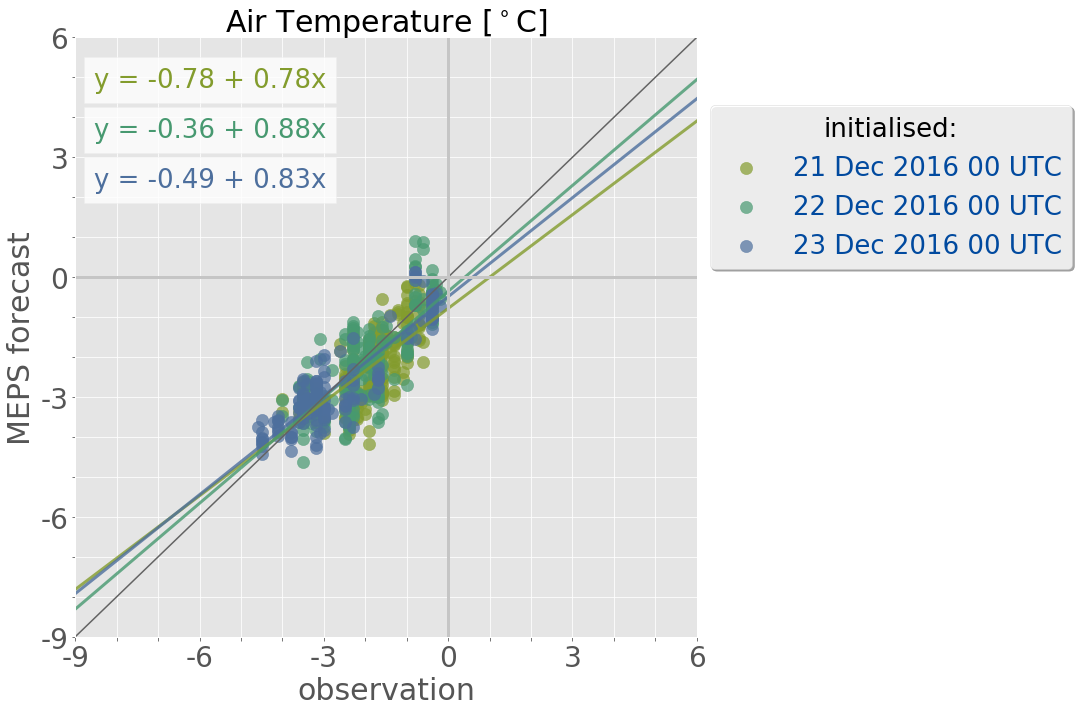
\includegraphics[trim={25.cm 15.5cm 0cm 3.6cm},clip,
    width=0.8\textwidth]{./fig_sfc_temp/obs_model_20161221_23_00}
     \end{subfigure}
     \begin{subfigure}[b]{0.49\textwidth}
     	\centering
     	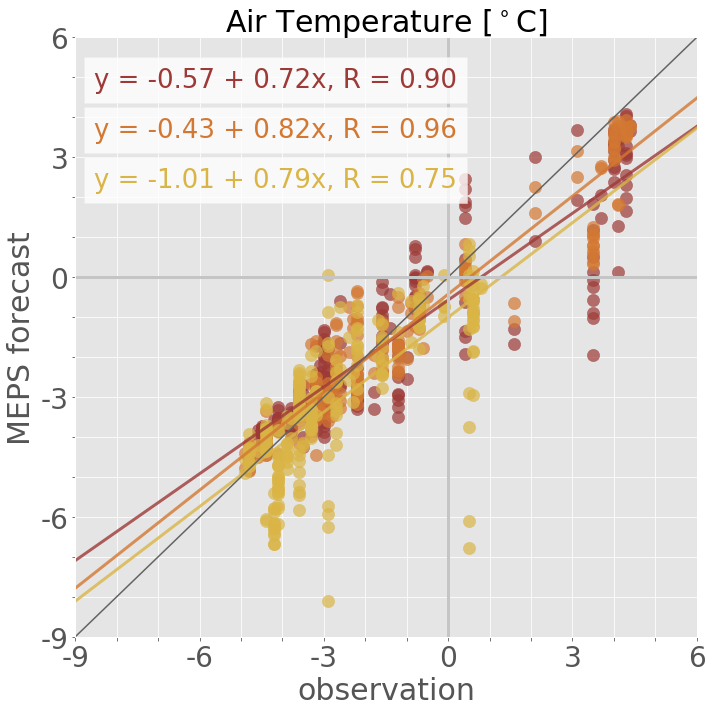
\includegraphics[trim={25.cm 15.5cm 0cm 3.6cm},clip,
    width=0.8\textwidth]{./fig_sfc_temp/obs_model_20161224_26_00}
    \end{subfigure}
\end{figure}
\begin{figure}\ContinuedFloat
     % sfc precip
	\begin{subfigure}[b]{0.49\textwidth}
     	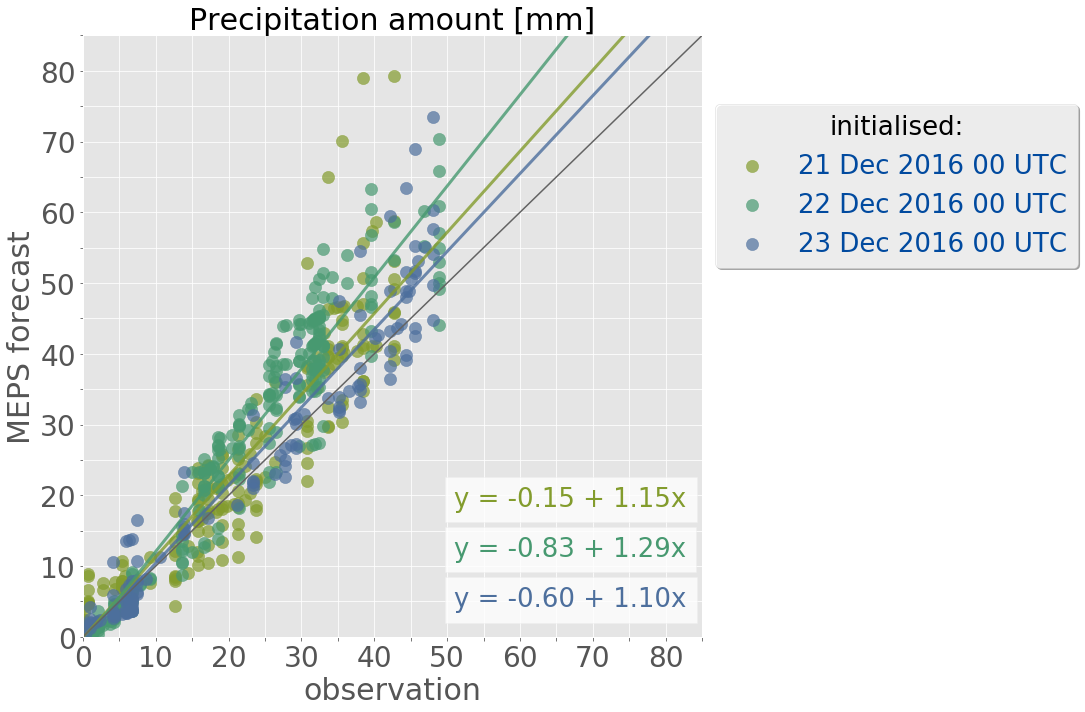
\includegraphics[trim={0.cm 0cm 12.5cm 0cm},clip,
    width=\textwidth]{./fig_sfc_precip/obs_model_20161221_23_00}
     	\caption{}\label{fig:scat:precip2123}
     \end{subfigure}
     %
	\begin{subfigure}[b]{0.49\textwidth}
     	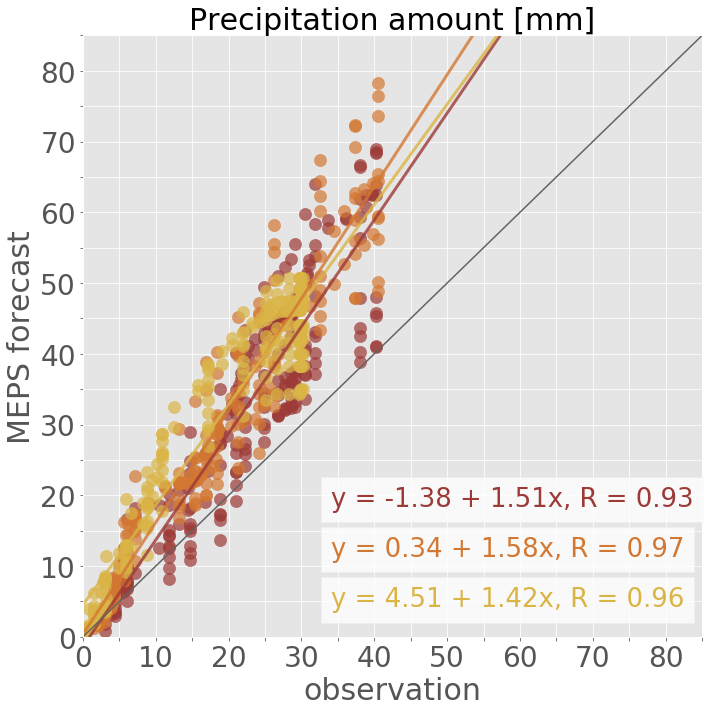
\includegraphics[trim={0.cm 0cm 12.5cm 0cm},clip,
    width=\textwidth]{./fig_sfc_precip/obs_model_20161224_26_00}
     	\caption{}\label{fig:scat:precip2426}
     \end{subfigure}
     % label
     \begin{subfigure}[b]{0.49\textwidth}
     	\centering
     	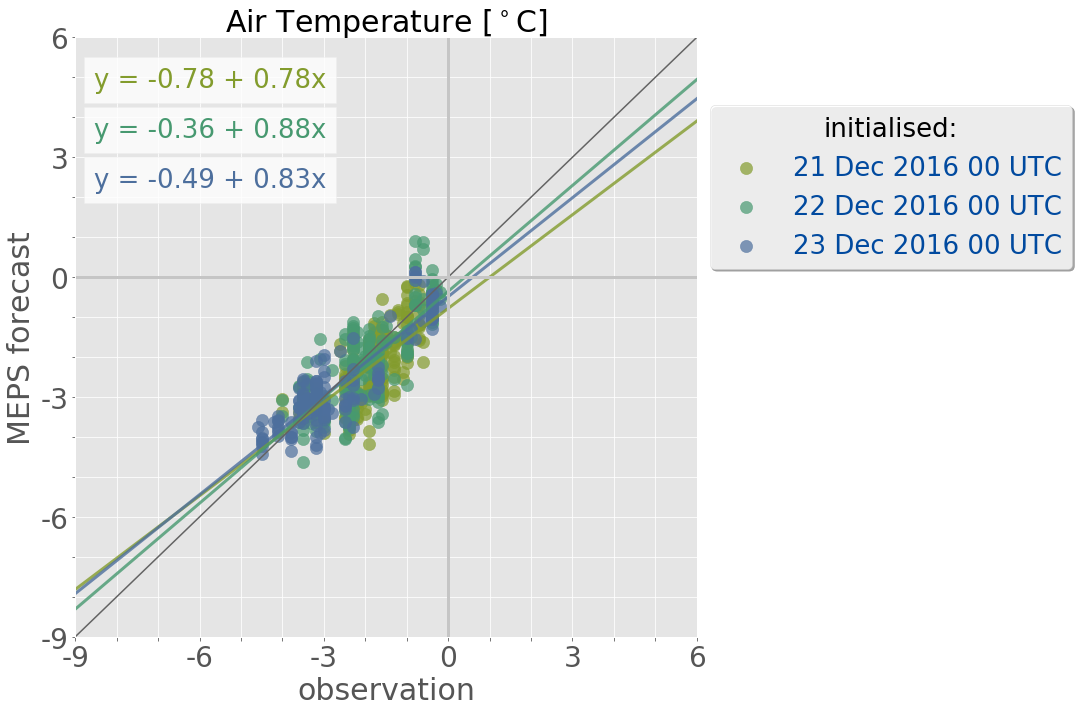
\includegraphics[trim={25.cm 15.5cm 0cm 3.6cm},clip,
    width=0.8\textwidth]{./fig_sfc_temp/obs_model_20161221_23_00}
     \end{subfigure}
     \begin{subfigure}[b]{0.49\textwidth}
     	\centering
     	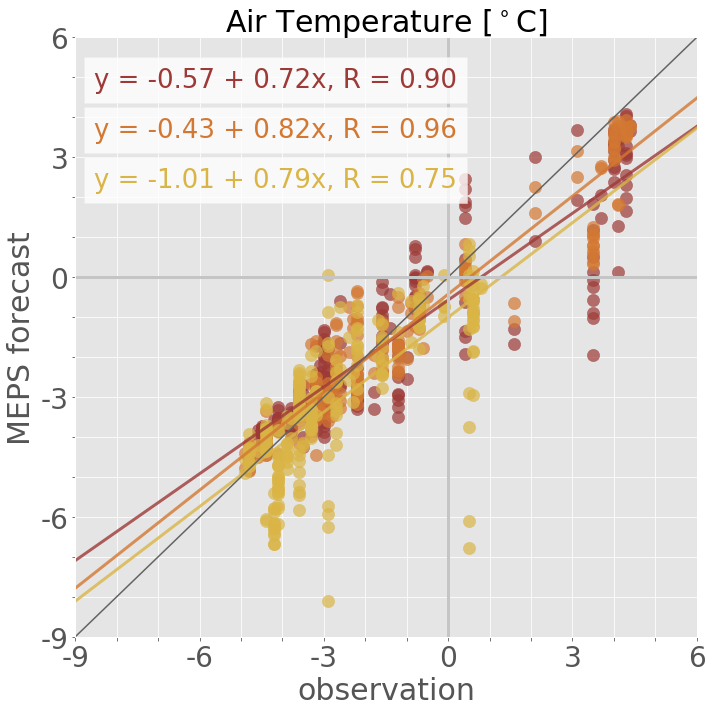
\includegraphics[trim={25.cm 15.5cm 0cm 3.6cm},clip,
    width=0.8\textwidth]{./fig_sfc_temp/obs_model_20161224_26_00}
     \end{subfigure}
     \caption{\SI{48}{\hour} scatter plots for surface observations and ensemble forecasts initialised for \SIrange{21}{23}{\dec} (left column, \protect\subref{fig:scat:pres2123}, \protect\subref{fig:scat:temp2123}, \protect\subref{fig:scat:wd2123}, \protect\subref{fig:scat:ws2123}, \protect\subref{fig:scat:precip2123}) and  for \SIrange{24}{26}{\dec} (right column, \protect\subref{fig:scat:pres2426}, \protect\subref{fig:scat:temp2426}, \protect\subref{fig:scat:wd2426}, \protect\subref{fig:scat:ws2426}, \protect\subref{fig:scat:precip2426}). Upper panel sea level pressure, second \SI{2}{\metre} air temperature, third and forth \SI{10}{\metre} wind direction and speed, respectively, and lowest panel precipitation amount.}\label{fig:scat:obs_meps}
\end{figure}
%%%%%%%%%%%%%%%%%%%%%%%%%%%%%%%%%%%%%%%%%%%%%%
\\
The comparison between the ECMWF analysis shows, that the ensemble member forecast system MEPS covers the prediction of large scale phenomena like frontal boundaries and liquid precipitation at the surface. \Cref{fig:scat:obs_meps} shows the correlation between the observations and the \SI{48}{\hour} forecast. Each variable presents the regression line  for each day and all ensemble members compared to the observations at Haukeliseter.
\\
Sea level pressure has the best correlation under all variables. The best agreement shows on \SI{26}{\dec} when the Christmas storm made landfall and dissipates after the passage of the occluded front at \SI{16}{\UTC}. \cite{dahlgren_comparison_2013} showed that by mixing in large scale information from the boundary condition (ECMWF) into the regional model, the forecast for sea level pressure will be improved. The comparison with observational data showed a declination of forecasts after \SI{24}{\hour}. 
Since the pressure values are in good agreement with the observations are assumed that on \SI{25}{\dec} the warm front did not pass through at Haukeliseter. 
\\
The warm sector passing through on \SI{25}{\dec} was predicted by MEPS and observed at the station. Comparing \Cref{fig:scat:temp2426} shows a moderate correlation between observation and \SI{48}{\hour} forecast. MEPS underestimated the observed temperature, but it estimated it at the correct time. In \cite{muller_arome-metcoop:_2017} it states that after winter 2012 was the temperature bias negative. \Cref{fig:bias:temp} shows for \SIlist{23;26}{\dec} positive as well as negative biases for the individual members. The \SI{25}{\dec}, where the warm sector was observed shows a negative bias, underestimating the temperature when compared to the observation. The mean error for the Norwegian model domain of AROME-MetCoOP estimated by \cite{muller_arome-metcoop:_2017} is smaller than \SI{1.8}{\kelvin} for the surface temperature in December 2014. The forecasts for \SIlist{23;25;26}{\dec} show mean absolute error values of up to \SIlist{0.61;0.77;1.44}{\kelvin}. This shows a good predictability for temperatures of the event. 
\\
According to \cite{muller_arome-metcoop:_2017} are large wind speeds significantly better simulated for AROME-MetCoOp compared to ECMWF's forecast. The wind speeds between \SIrange{3}{13}{\mPs} agreed with observed and forecasted values for the 2014/2015 season where for higher values the accuracy decreased. Mean absolute errors were below \SI{2}{\mPs} for December 2014. 
\\
\Cref{fig:scat:ws2123} and \subref{fig:scat:ws2426} show indeed higher values than the observations at Haukeliseter. The mean absolute error for the Christmas storm is higher at all days. From the three days with frontal passages the \SI{23}{\dec} shows the highest mean absolute error of \SI{6.5}{\mPs}, more than three times as high as the monthly averaged value from \cite{muller_arome-metcoop:_2017}. Their study case in February 2015 showed a large difference between AROME-MetCoOp and ECMWF. While the wind direction of MEPS has a good agreement shows the wind speed larger values over all days. Although MEPS includes ten perturbed ensemble members the insufficiency of AROME-MetCoOp too high wind prediction in extreme situations is not resolved. The regional model wind prediction is still dependent on the intensity of the storm. As \cite{muller_arome-metcoop:_2017} also mentioned are higher wind speeds in general better forecasted in AROME-MetCoOp than in ECMWF. 
\\
Haukeliseter is a measurement site exposed to high wind speeds \citep{wolff_measurements_2013,wolff_derivation_2015} it shows in the results, the positive impact of a high resolution forecast model since it is able to estimate larger scale features. In general were surface parameters well forecasted, only wind wind speed and precipitation accumulation showed overestimation in MEPS. Wind speeds forecasted higher than observations, is probably related to the weakness of wind speed prediction already known from the previous operational model AROME-MetCoOp. On the \SIlist{25;26}{\dec} MEPS also overestimated the precipitation amount at the surface. This will be further discussed in \Cref{sec:sfc_acc}.
%%%%%%%%%%%%%%%%%%%%%%%%%%%%%%%%%%%%%%%%%%%%%%%%%%%%%%%%%%%%%%%%%%%%%%%%%%

%%%%%%%%%%%%%%%%%%%%%%%%%%%%%%%%%%%%%%%%%%%%%%%%%%%%%%%%%%%%%%%%%%%%%%%%%%
%%%%%%%%% Local affects %%%%%%%%%%%%%%
\section{Orographic influence on precipitation}
%%%%%%%%%%%%%%%%%%%%%%%%%%%%%%%%%%%%%%%%%%%%%%%%%%%%%%%%%%%%%%%%%%%%%%%%%%

%%%%%%%%%%%%%%%%%%%%%%%%%%%%%%%%%%%%%%%%%%%%%%%%%%%%%%%%%%%%%%%%%%%%%%%%%
%%%%%%%% Relationship between wind and surface accumulation %%%%%%%%%%%%%%
\section{Relation between surface precipitation amount and wind}\label{sec:sfc_acc}
%%%%%%%%%%%%%%%%%%%%%%%%%%%%%%%%%%%%%%%%%%%%%%%%%%%%%%%%%%%%%%%%%%%%%%%%%






%%%%%%%%%%%%%%%%%%%%%%%%%%%%%%%%%%%%%%%%%%%%%%%%%%%%%%%%%%%%%%%%%%%%%%%%%


%%%%%%%%%%%%%%%%%%%%%%%%%%%%%%%%%%%%%%%%%%%%%%%%%%%%%%%%%%%%%%%%%%%%%%%%%
%%%%%%%% surface %%%%%%%%%%%%%%
% !TeX spellcheck = en_GB
%%%%%%%%%%%%%%%%%%%%%%%%%%%%%%%%%%%%%%%%%%%%%%%%%%%%%%%%%%%%%%%%%%%%%%%%%
%%%%%%%% large scale phenomena vertical ? %%%%%%%%%%%%%%
\section{Observation of large scale weather phenomena in the vertical}%\label{sec:res:verticalSWC}
\label{sec:res:large_scale_vert}
%%%%%%%%% image reflectivity %%%%%%%%%%%%%%
\begin{figure}[h!]
	\centering
	% 23/12
	\begin{subfigure}[t]{\textwidth}
		\centering
		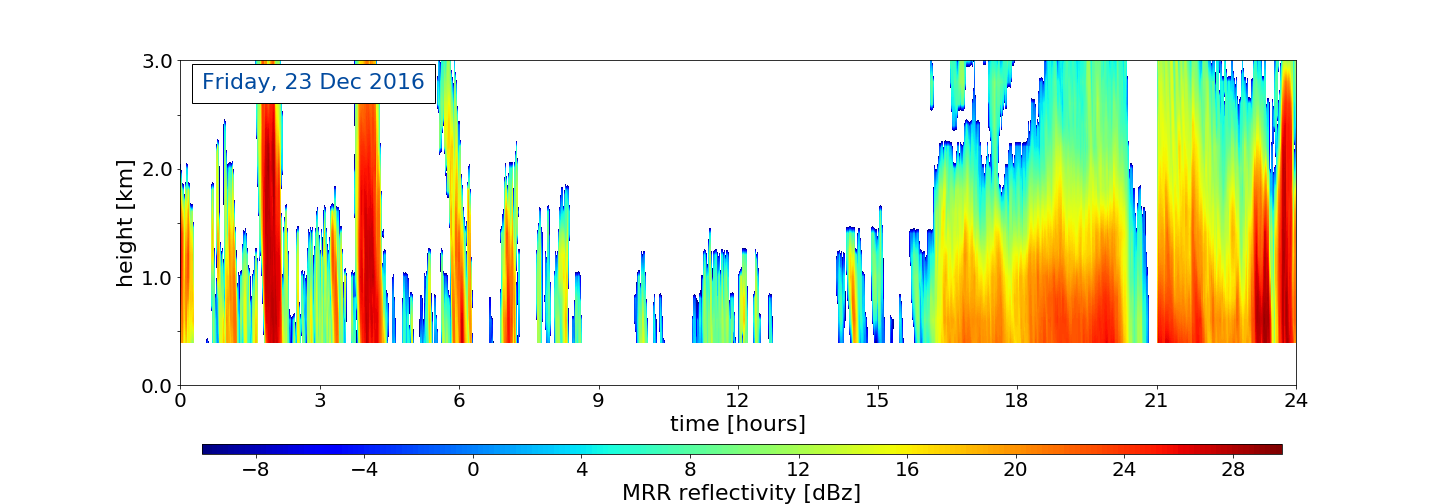
\includegraphics[trim={4.cm 2.5cm 4.5cm 1.5cm},clip,width=0.9\textwidth]{./fig_MRR_refl/MRR_20161223}
		\caption{}\label{fig:ret:refl23}
	\end{subfigure}
	% 25/12
	\begin{subfigure}[t]{\textwidth}
		\centering
		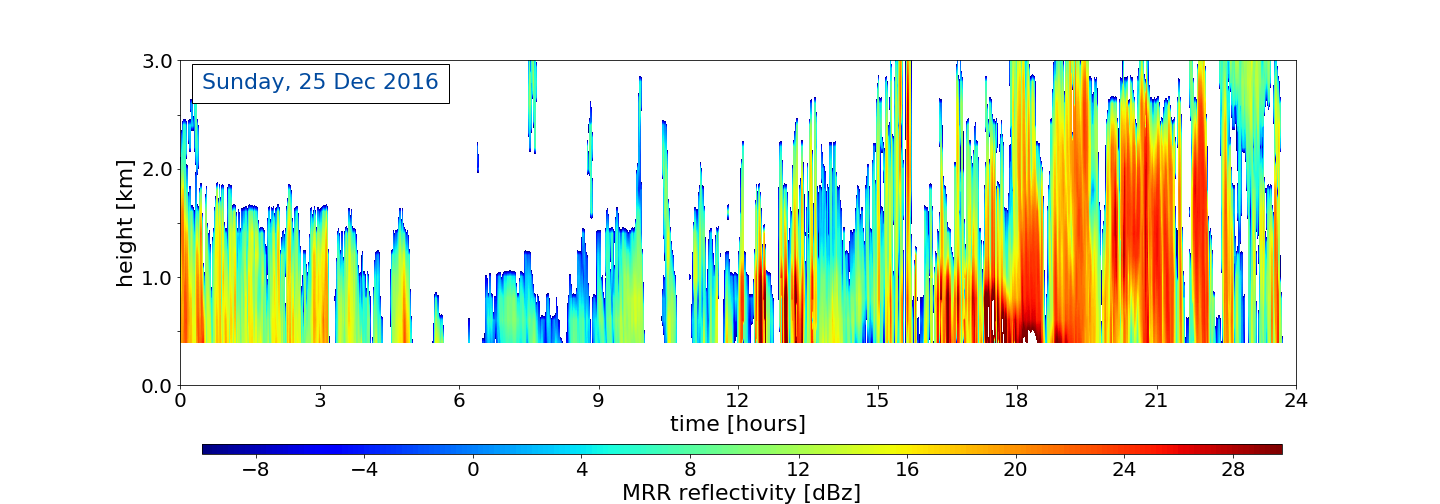
\includegraphics[trim={4.cm 2.5cm 4.5cm 1.5cm},clip,width=0.9\textwidth]{./fig_MRR_refl/MRR_20161225}
		\caption{}\label{fig:ret:refl25}
	\end{subfigure}
	% 26/12
	\begin{subfigure}[t]{\textwidth}
		\centering
		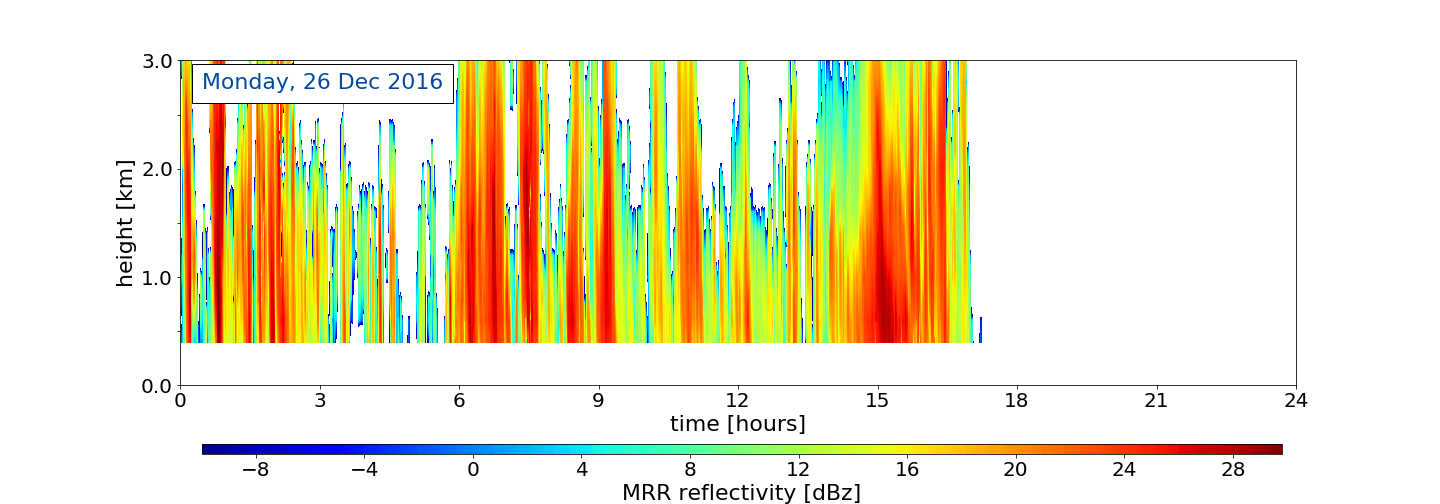
\includegraphics[trim={4.cm 2.5cm 4.5cm 1.5cm},clip,width=0.9\textwidth]{./fig_MRR_refl/MRR_20161226}
		\caption{}\label{fig:ret:refl26}
	\end{subfigure}
	% label
	\begin{subfigure}[t]{\textwidth}
		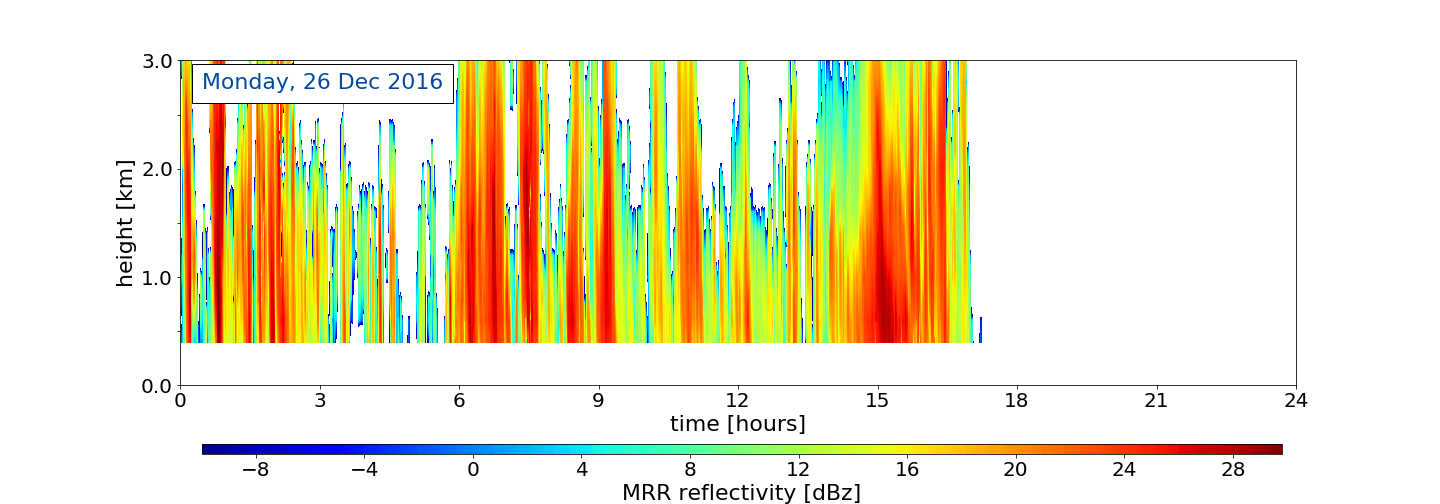
\includegraphics[trim={6.5cm 0cm 5.3cm 15.5cm},clip,width=\textwidth]{./fig_MRR_refl/MRR_20161226}
	\end{subfigure}
	\caption{MRR reflectivity for the days when a front or an occlusion passed through at Haukeliseter. \SI{}{\decibel Z} reflectivity according to the colour bar, with weaker precipitation in blue and more intense precipitation in red. \protect\subref{fig:ret:refl23}: Friday, \SI{23}{\dec}, \protect\subref{fig:ret:refl25}: Sunday, \SI{25}{\dec}, and \protect\subref{fig:ret:refl26}: Monday, \SI{26}{\dec}.}\label{fig:ret:refl}
\end{figure}
%%%%%%%%%%%%%%%%%%%%%%%%%%%%%%%%%%%%%%%%%%%%%%%%%%%%%%%%%%%%%%%%%%%%%%%%%
\noindent
Frontal boundary passages were observed at the surface several times throughout the extreme storm in December 2016. MEPS is able to predict the large scale features and related surface changes for initialisation more than \SI{24}{\hour} before (\Cref{sec:res:large_scale_sfc}). In winter 2016 three additional instruments were installed to estimate the vertical snow water content at Haukeliseter. This unique approach gives the opportunity to compare the vertical forecasts of SWC to vertical solid precipitation observations. As far as the author knows is there no study on this particular topic about the verification of vertical ensemble member prediction models with observations.
%\\
\\
\Cref{fig:ret:refl} shows the reflectivity from the MRR at Haukeliseter for \SIlist{23;25;26}{\dec}. Passages of occluded fronts and a warm sector were observed on \SIlist{23;26;25}{\dec}, respectively. \Cref{fig:ret:refl26} presents only values until \SI{17}{\UTC}, because of the temperature change and hence a precipitation shift followed liquid drops freezing on the MRR dish and the signal got attenuated. 
\\
The transit of the boundary is shown in \Cref{fig:ret:refl} by the more consistent structure of a storm with higher reflectivity values. 
While on \SIlist{23;26}{\dec} the reflectivity did not pass values larger than \SI{28}{\decibel Z} shows \Cref{fig:ret:refl25} high reflectivity values larger than \SI{30}{\decibel Z} (compare for approximation \Cref{tab:ref_values}). These high values indicate the observation of possible liquid precipitation. Images from the MASC were able to verify observed liquid drops during \SIrange{12}{21}{\UTC} (\Cref{fig:res:obs_masc}). 
\\
On \SI{23}{\dec} allow the surface observations to assume that the occluded front passed through between \SIrange{12}{21}{\UTC} (\Cref{fig:res:sfc_pres23}, \subref{fig:res:sfc_temp23}, \subref{fig:res:sfc_wd23}). The vertical observations at Haukeliseter show intense reflectivity and therefore more intense precipitation after \SI{16}{\UTC} (\Cref{fig:ret:refl23}). Another occlusion passed through on \SI{26}{\dec} shortly before \SI{15}{\UTC} which lasted until \SI{21}{\UTC} indicated by a more consistent storm structure in \Cref{fig:ret:refl26} around \SI{15}{\UTC}. The high reflectivity on both days shows the passage of the occlusion and the associated precipitation. The wind on \SI{23}{\dec} was from the south, upslope (\Cref{fig:res:sfc_wd23}, \Cref{fig:site:kartverket}) which led to a more consistent storm structure. On \SI{25}{\dec} indicate \Cref{fig:res:sfc_wd25} and \subref{fig:res:sfc_ws25} strong wind observations from the west which led to a consistent, but shorter storm structure in \Cref{fig:ret:refl25} at \SI{15}{\UTC}. The orographic influenced wind and therefore a possible relation to the precipitation will be further assessed in \Cref{sec:res:oro_infl}. 
\\
\\
\Cref{fig:SWC} presents the reflectivity from the MRR and the snow water content retrieved from the reflectivity as well as the \SI{48}{\hour} forecast values. Minutely MRR reflectivity and retrieved snow water content can be seen in \Cref{fig:SWC:ret_22}, \subref{fig:SWC:ret_23}, \subref{fig:SWC:ret_25}, and \subref{fig:SWC:ret_26}. \Cref{fig:SWC_EM:22}, \subref{fig:SWC_EM:23}, \subref{fig:SWC_EM:25}, \subref{fig:SWC_EM:26} show in the upper panel the hourly averaged values from the retrieved SWC and in the lower panel the ensemble mean of the instantaneous forecast values every hour over all ensemble member.   
Three hourly averaged retrieved values are then presented in the upper panel of \Cref{fig:SWC3h:22}, \subref{fig:SWC3h:23}, \subref{fig:SWC3h:25}, and \subref{fig:SWC3h:26}, the lower panel are the ensemble mean forecast values every three hours.
\\
\Cref{fig:SWC_EM:23} (lower panel) shows the one hourly averaged forecast values over all ensemble members, neglecting not existing values. Initialisations less than \SI{24}{\hour} before the event predict the consistent retrieved snowfall after \SI{16}{\UTC} (\Cref{fig:SWC:ret_23}, lower panel and \Cref{fig:SWC_EM:23}, upper panel). Even the three hourly averaged forecast values show a response on the occurrence of the storm (\Cref{fig:SWC3h:23}, lower panel). 
The duration of the passage is between \SIrange{16}{23}{\UTC} because of the longer time span is the prediction system able to estimate the snow water content. Forecasts initialised \SI{48}{\hour} prior predict also the consistent storm structure and therefore the passage of the front (\Cref{fig:SWC_EM:22}, \subref{fig:SWC3h:22}). 
\\
In general, is the forecasted instantaneous snow water content amount weaker than the retrieved values for predications on \SI{23}{\dec}. Hourly averages, only using the deterministic forecast and the first ensemble member show no occurrence of the occlusion passage on either day (\Cref{fig:SWC1h:22}, \subref{fig:SWC1h:23}, \subref{fig:SWC1h:25}, \subref{fig:SWC1h:26}). The variation of each ensemble member initialised on the respective day are given in \Cref{fig:EM09}. In \Cref{fig:EM09_22} is the prediction for the occlusion passage quite weak. 
%%%%%%%%% image SWC retrieval MEPS 22 %%%%%%%%%%%%%%
\begin{figure}[H]
	\centering
	% 23/12
	\begin{subfigure}[t]{\textwidth}
		\centering
		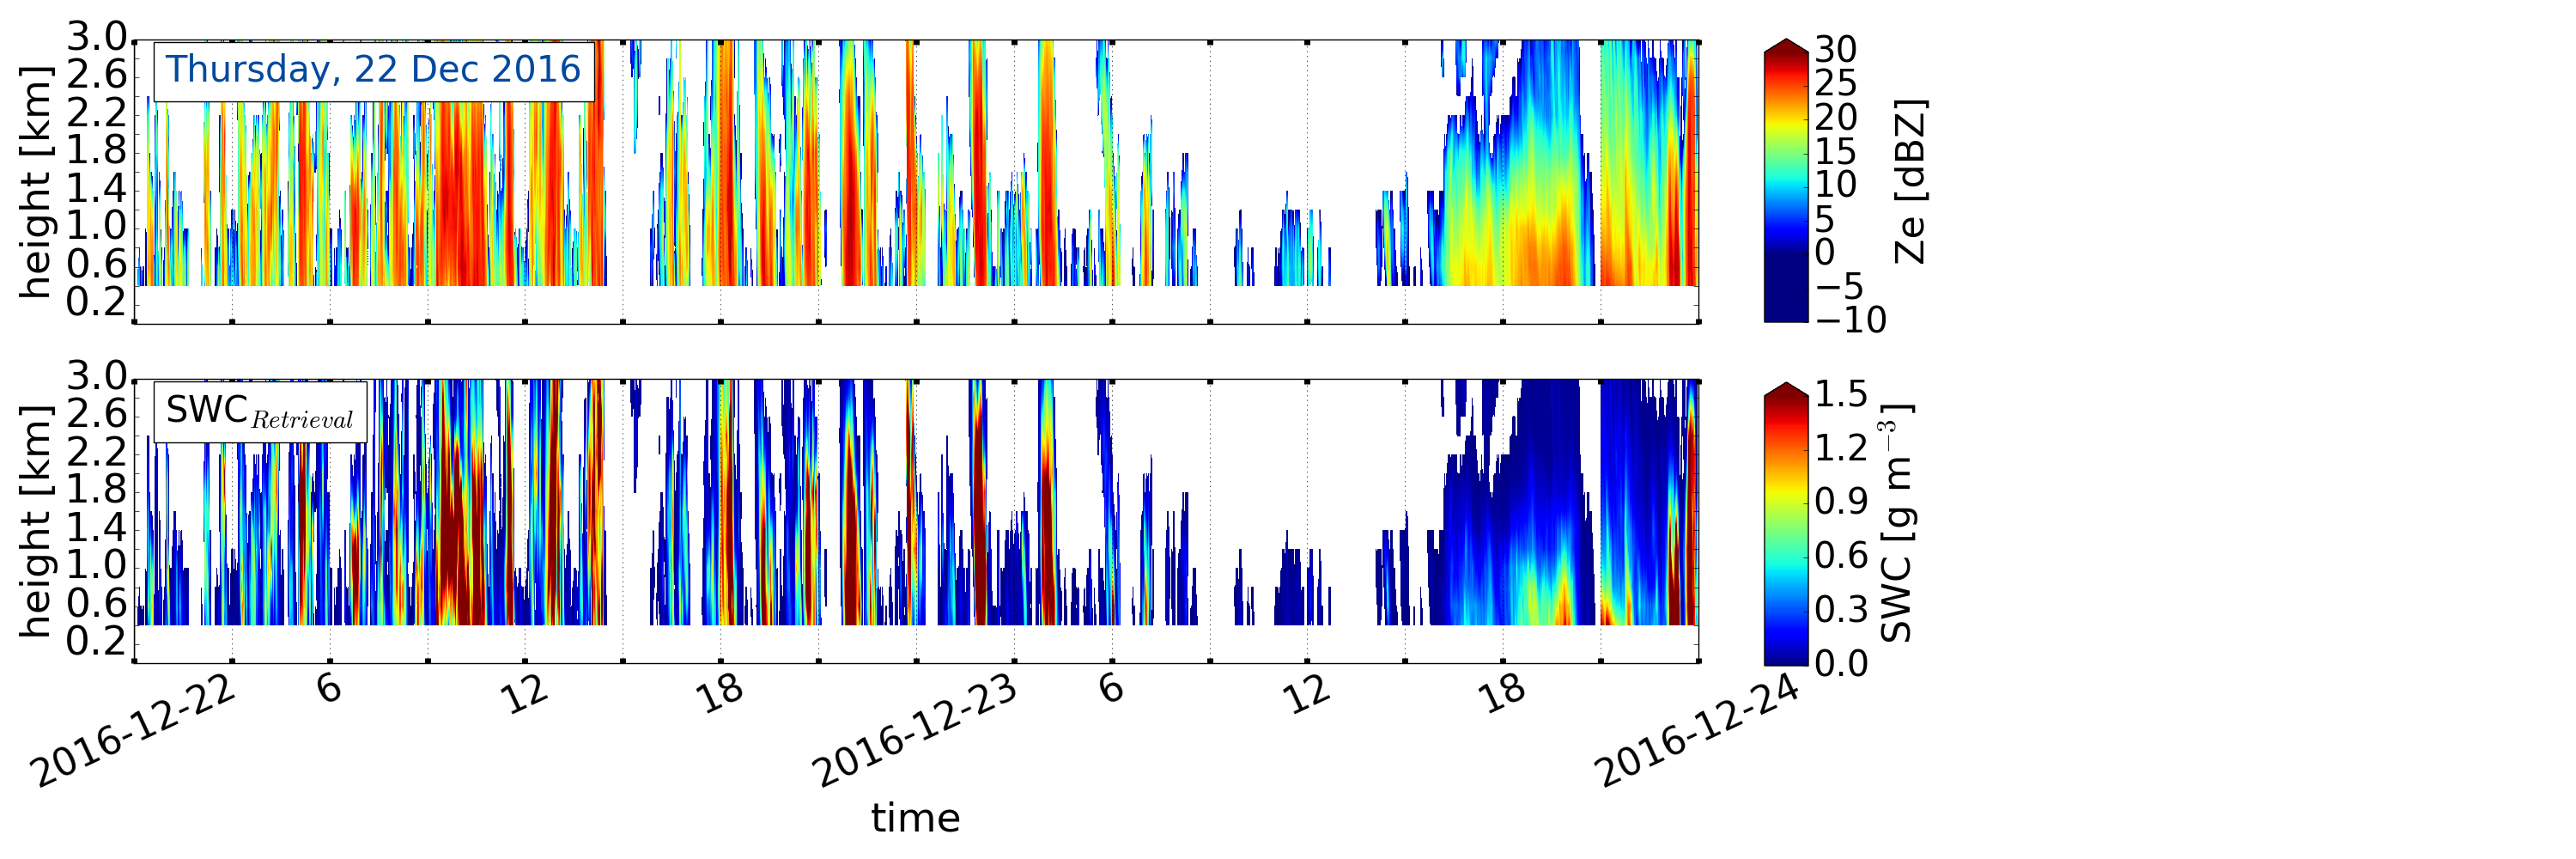
\includegraphics[trim={0.cm 2.2cm 19.cm 0.5cm},clip,width=0.9\textwidth]{./fig_obs_ret/20161222}
		\caption{}\label{fig:SWC:ret_22}
	\end{subfigure}
	% EM
	\begin{subfigure}[t]{\textwidth}
		\centering
		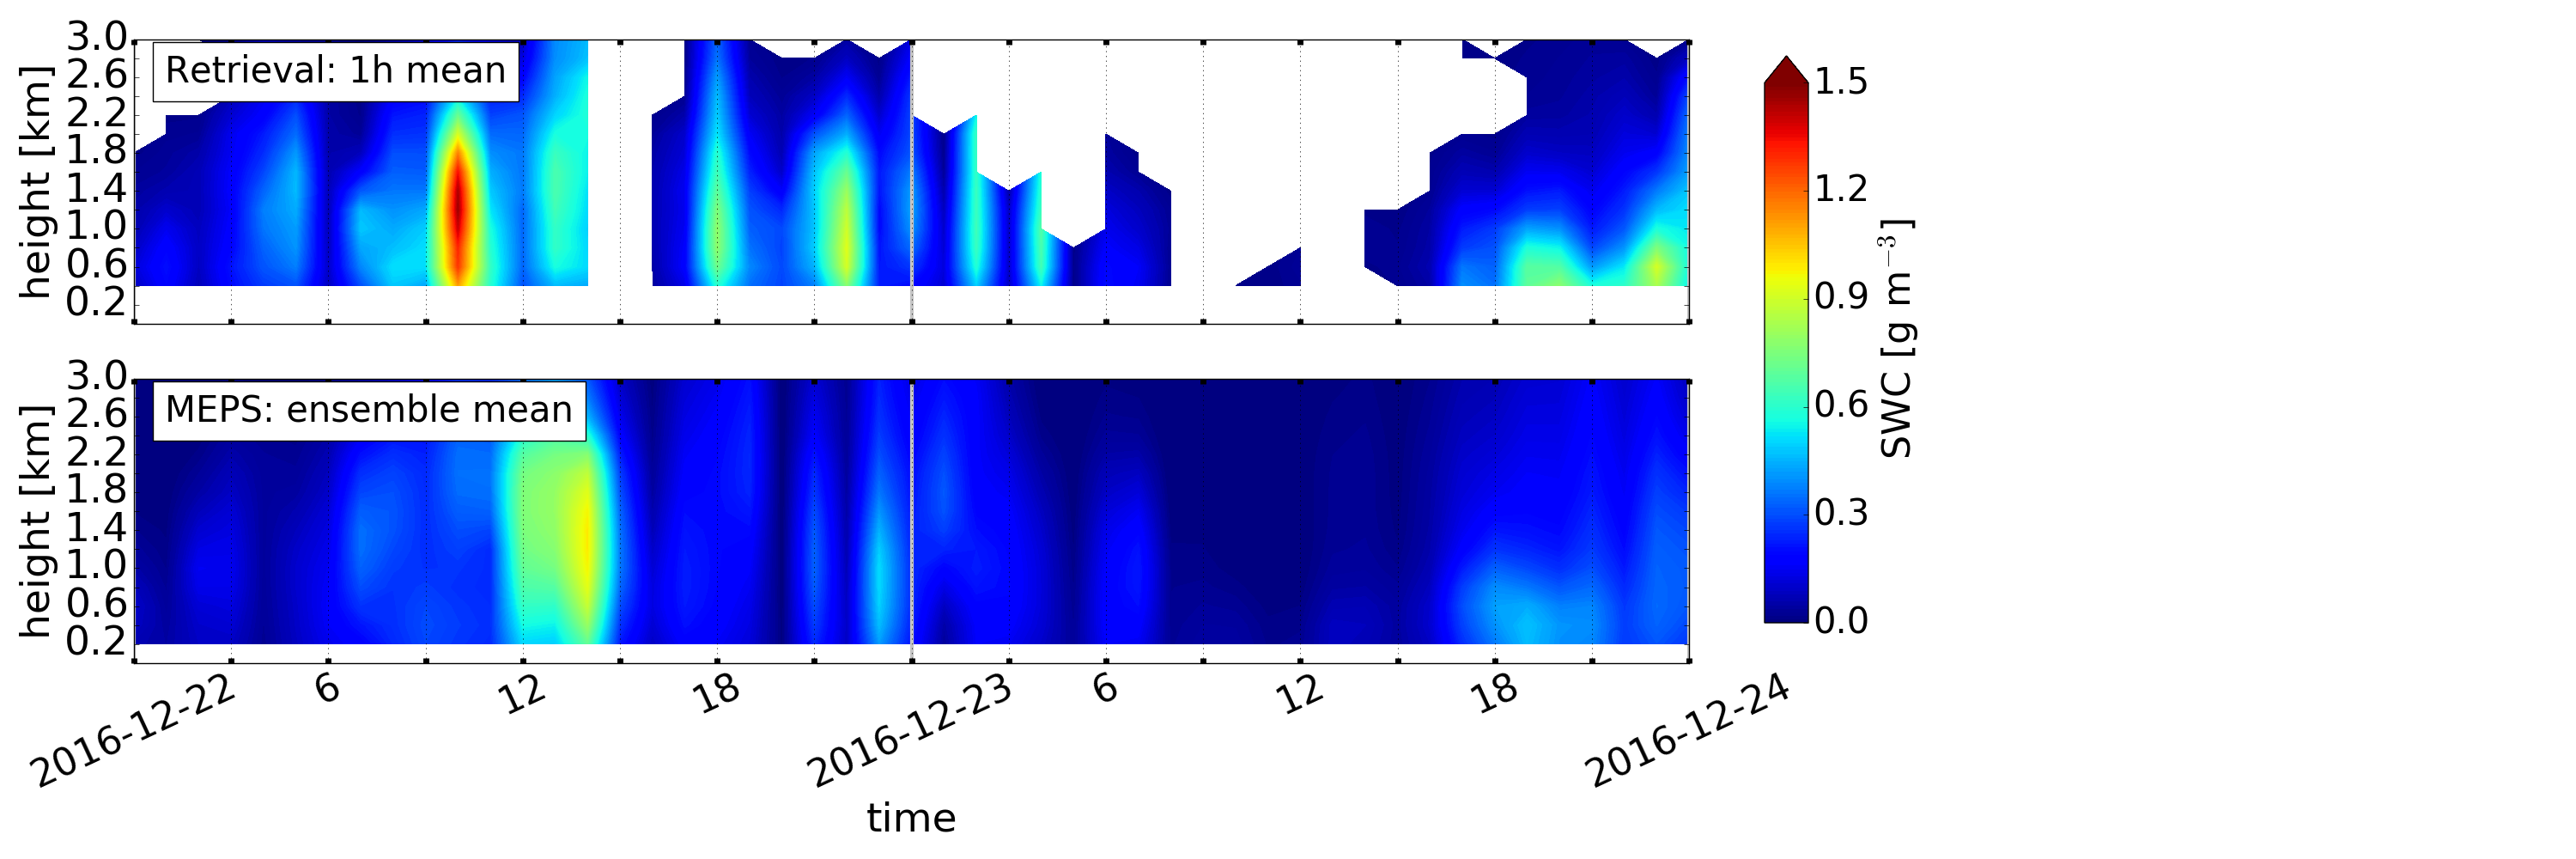
\includegraphics[trim={0.cm 2.2cm 19.cm 0.5cm},clip,width=0.9\textwidth]{./fig_vert_SWC_EM/20161222}
		\caption{}\label{fig:SWC_EM:22}
	\end{subfigure}
	% 3h
	\begin{subfigure}[t]{\textwidth}
		\centering
		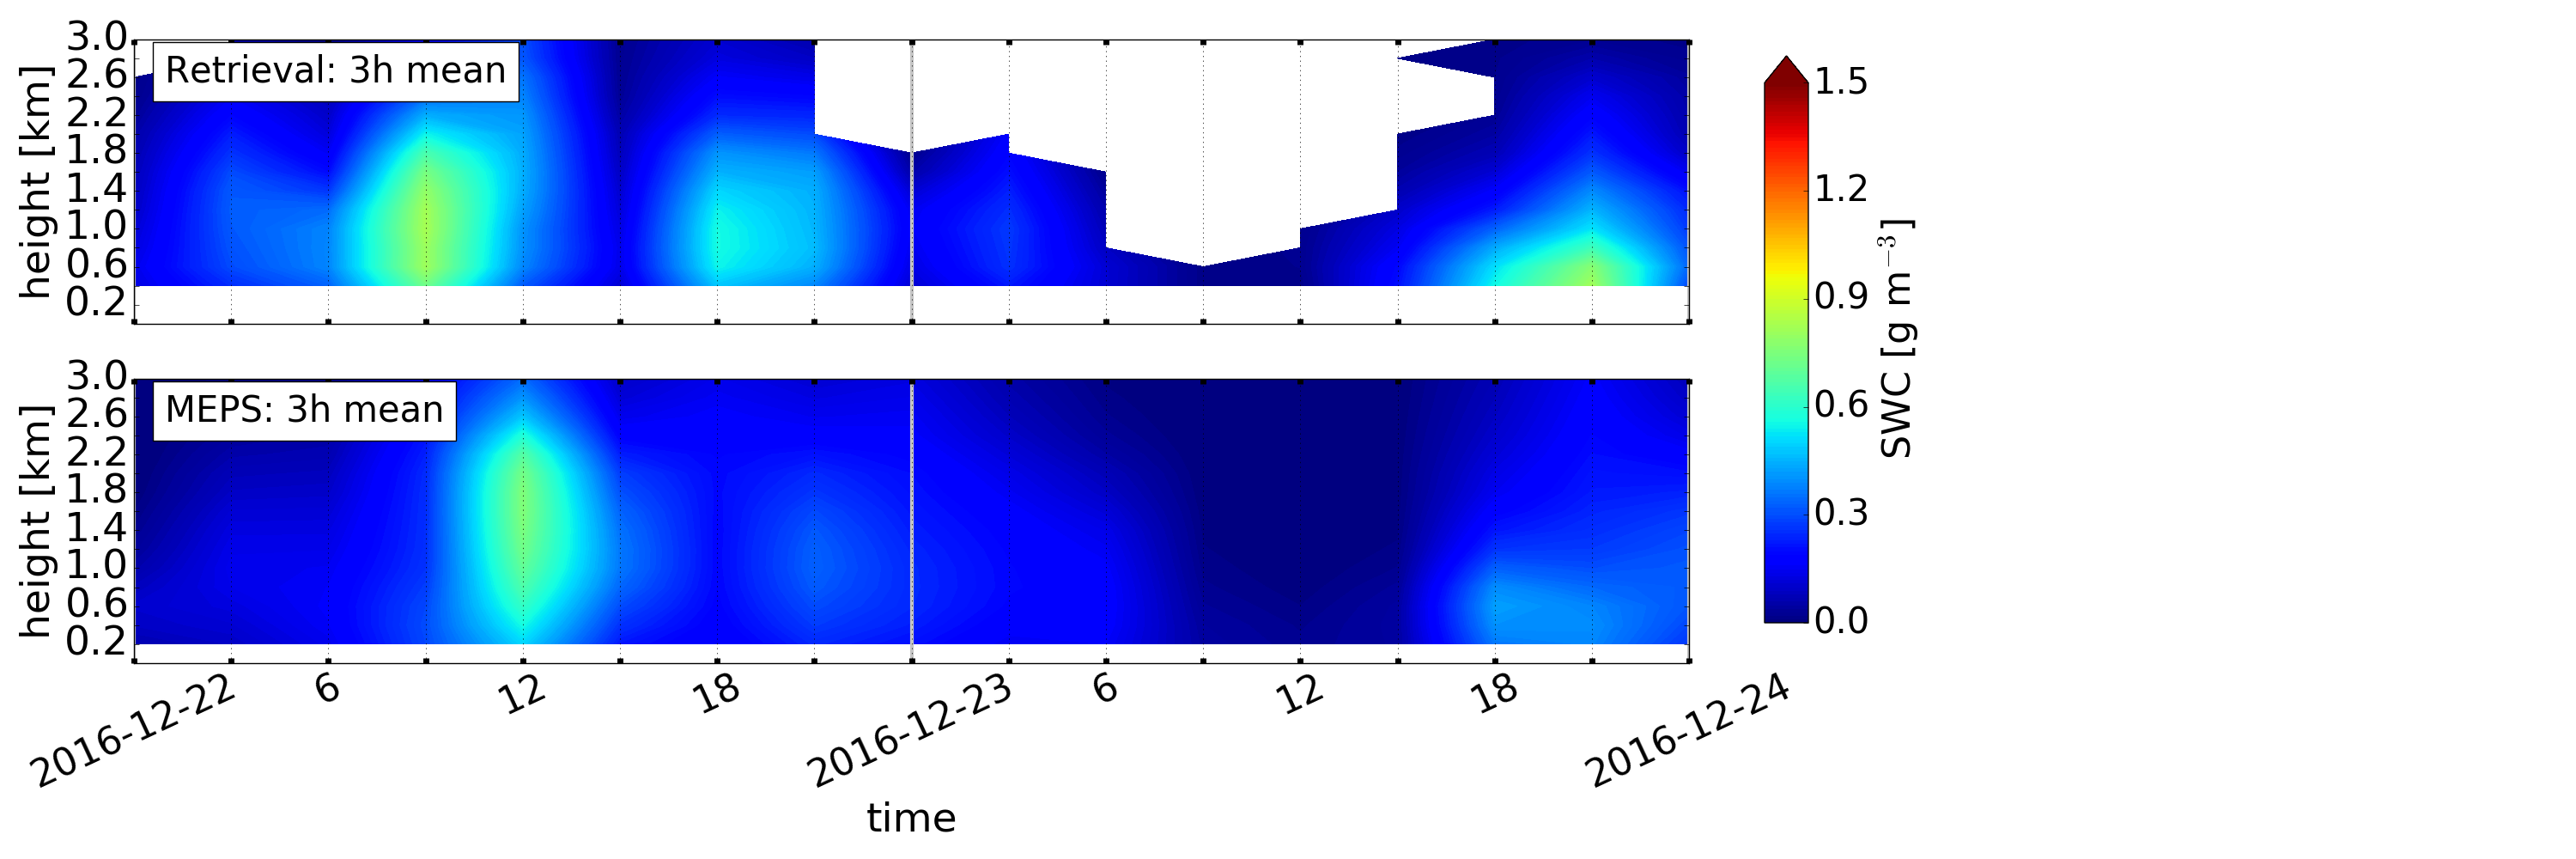
\includegraphics[trim={0.cm 0.8cm 19.cm 0.5cm},clip,width=0.9\textwidth]{./fig_vert_SWC_3h/20161222}
		\caption{}\label{fig:SWC3h:22}
	\end{subfigure}
	\caption{Initialisation \SIlist{22;23;25;26}{\dec} \SI{0}{\UTC}. 
		(\protect\subref{fig:SWC:ret_22},\protect\subref{fig:SWC:ret_23}, \protect\subref{fig:SWC:ret_25}, \protect\subref{fig:SWC:ret_26}) Upper panel: MRR reflectivity for \SI{48}{\hour}, lower panel minutely retrieved SWC. 
		(\protect\subref{fig:SWC_EM:22}, \protect\subref{fig:SWC_EM:23}, \protect\subref{fig:SWC_EM:25}, \protect\subref{fig:SWC_EM:26}) Upper panel: hourly averaged retrieved SWC, lower panel instantaneous hourly averaged forecast of all ensemble member SWC, neglecting missing values. 
		(\protect\subref{fig:SWC3h:22}, \protect\subref{fig:SWC3h:23}, \protect\subref{fig:SWC3h:25}, \protect\subref{fig:SWC3h:26}) Upper panel three hourly averaged retrieved SWC, lower panel instantaneous three hourly averaged forecast of all ensemble member SWC.   }\label{fig:ret:SWC}
\end{figure}
%%%%%%%%% image SWC retrieval MEPS 23 %%%%%%%%%%%%%%
\begin{figure}[H]\ContinuedFloat
	\centering
	% 23/12
	\begin{subfigure}[t]{\textwidth}
		\centering
		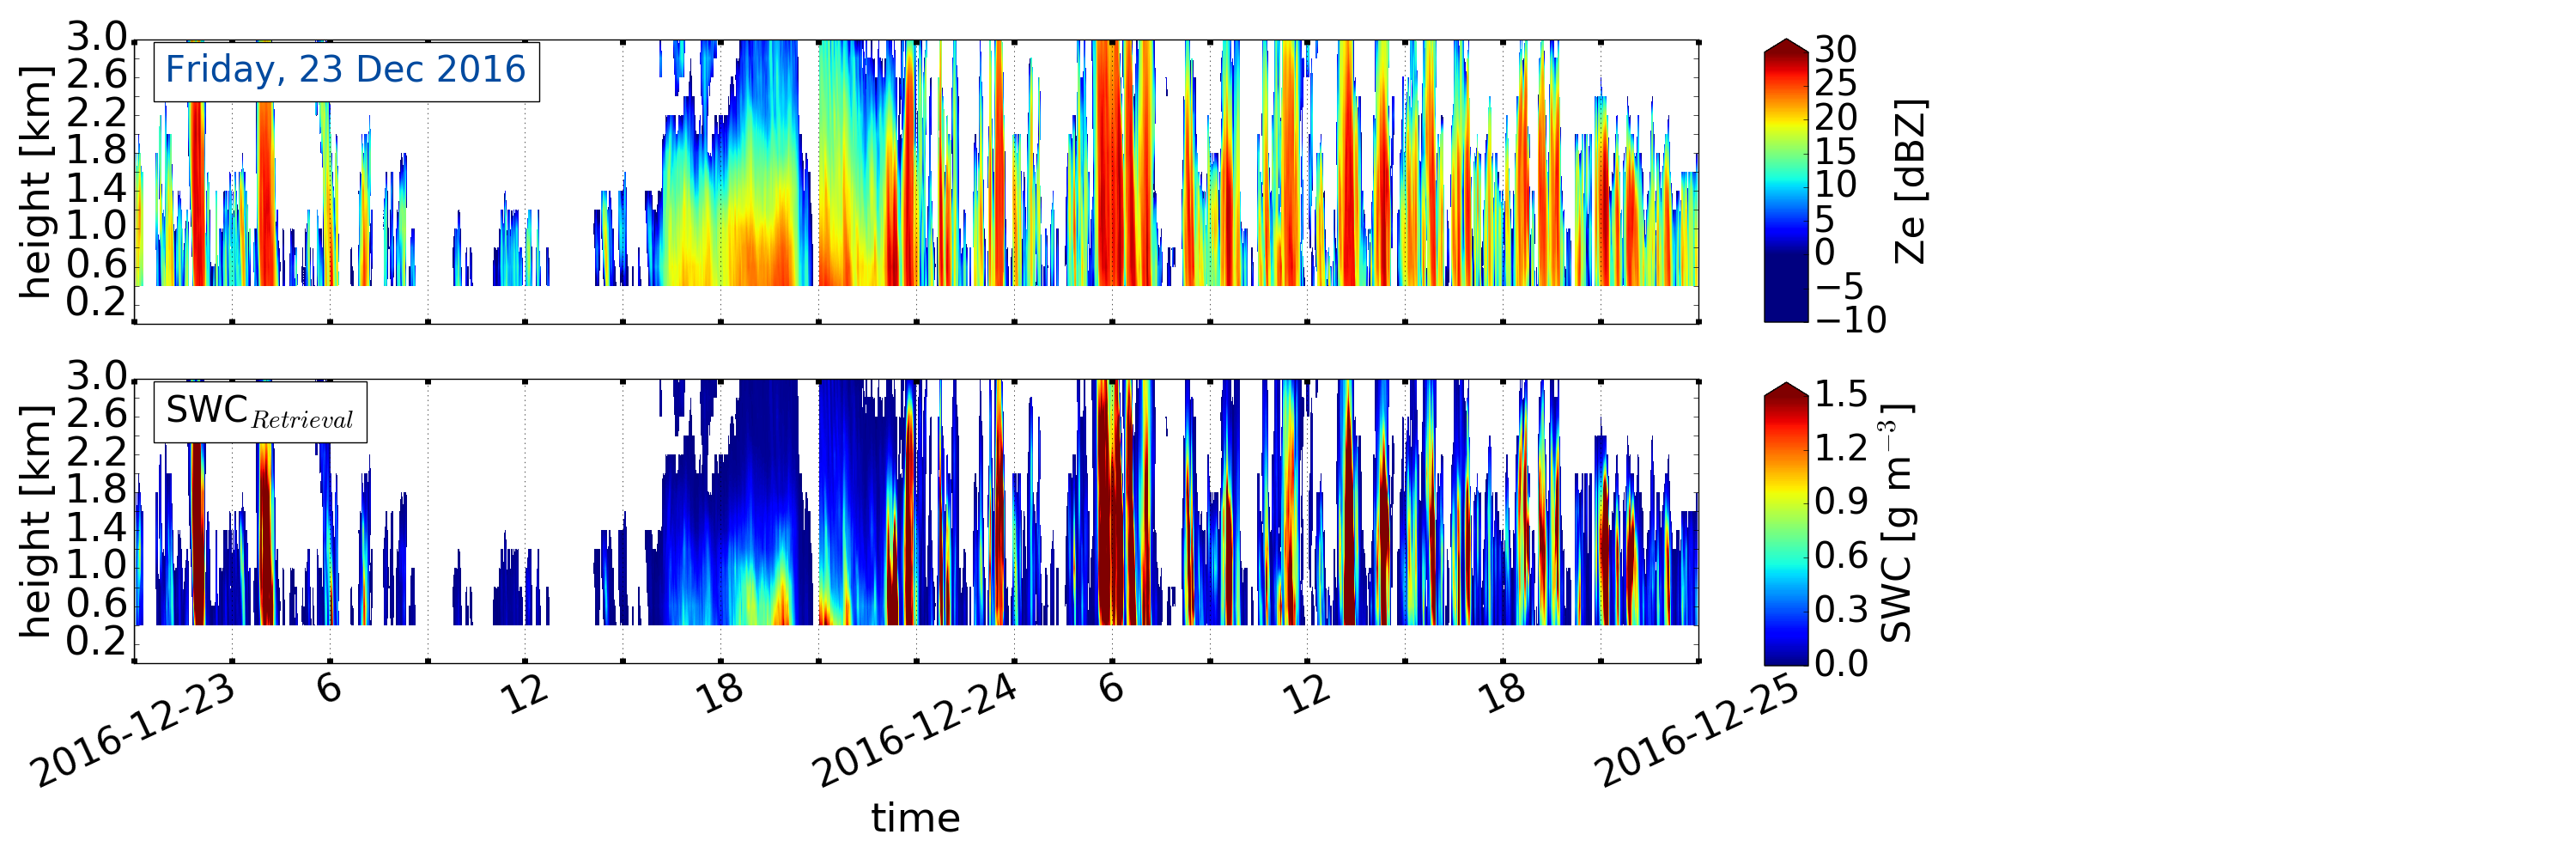
\includegraphics[trim={0.cm 2.2cm 19.cm 0.5cm},clip,width=0.9\textwidth]{./fig_obs_ret/20161223}
		\caption{}\label{fig:SWC:ret_23}
	\end{subfigure}
	% EM
	\begin{subfigure}[t]{\textwidth}
		\centering
		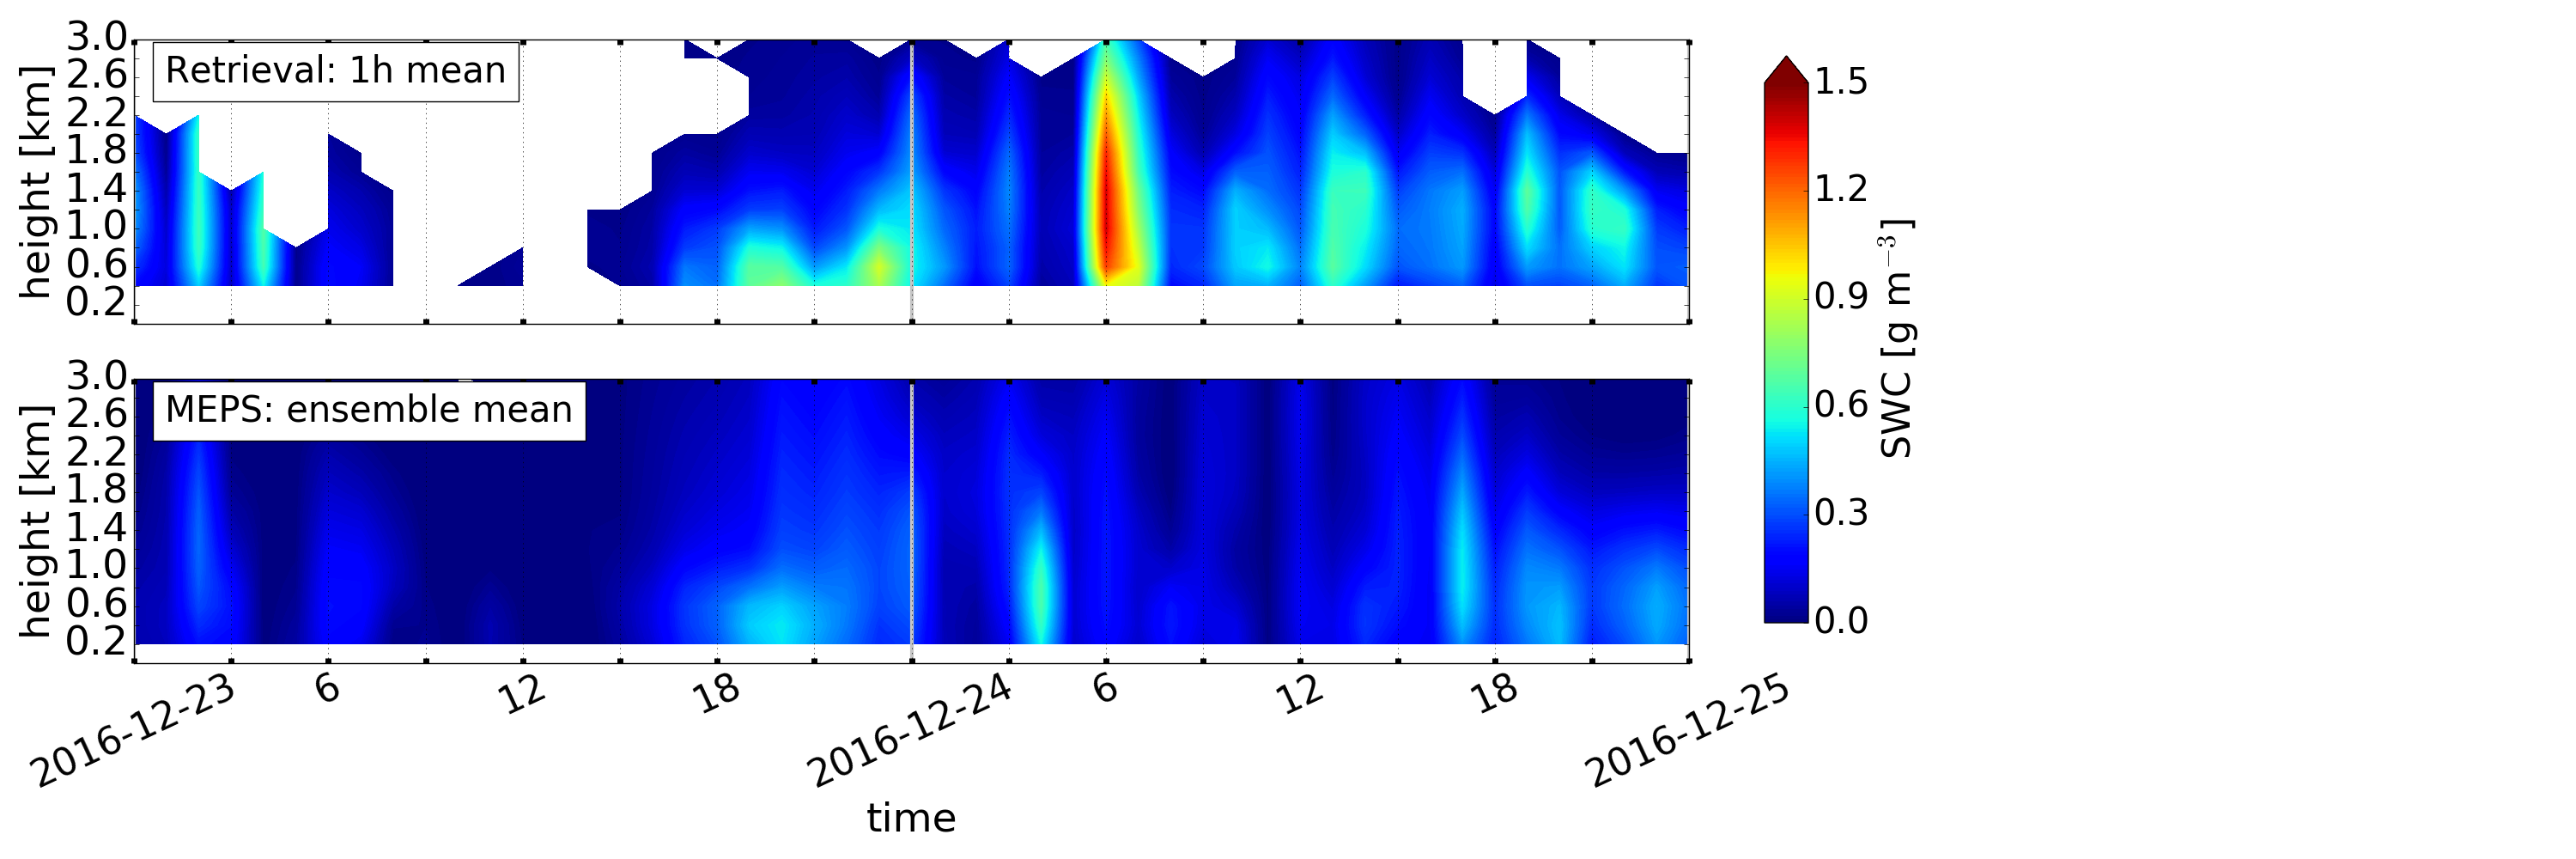
\includegraphics[trim={0.cm 2.2cm 19.cm 0.5cm},clip,width=0.9\textwidth]{./fig_vert_SWC_EM/20161223}
		\caption{}\label{fig:SWC_EM:23}
	\end{subfigure}
	% 3h
	\begin{subfigure}[t]{\textwidth}
		\centering
		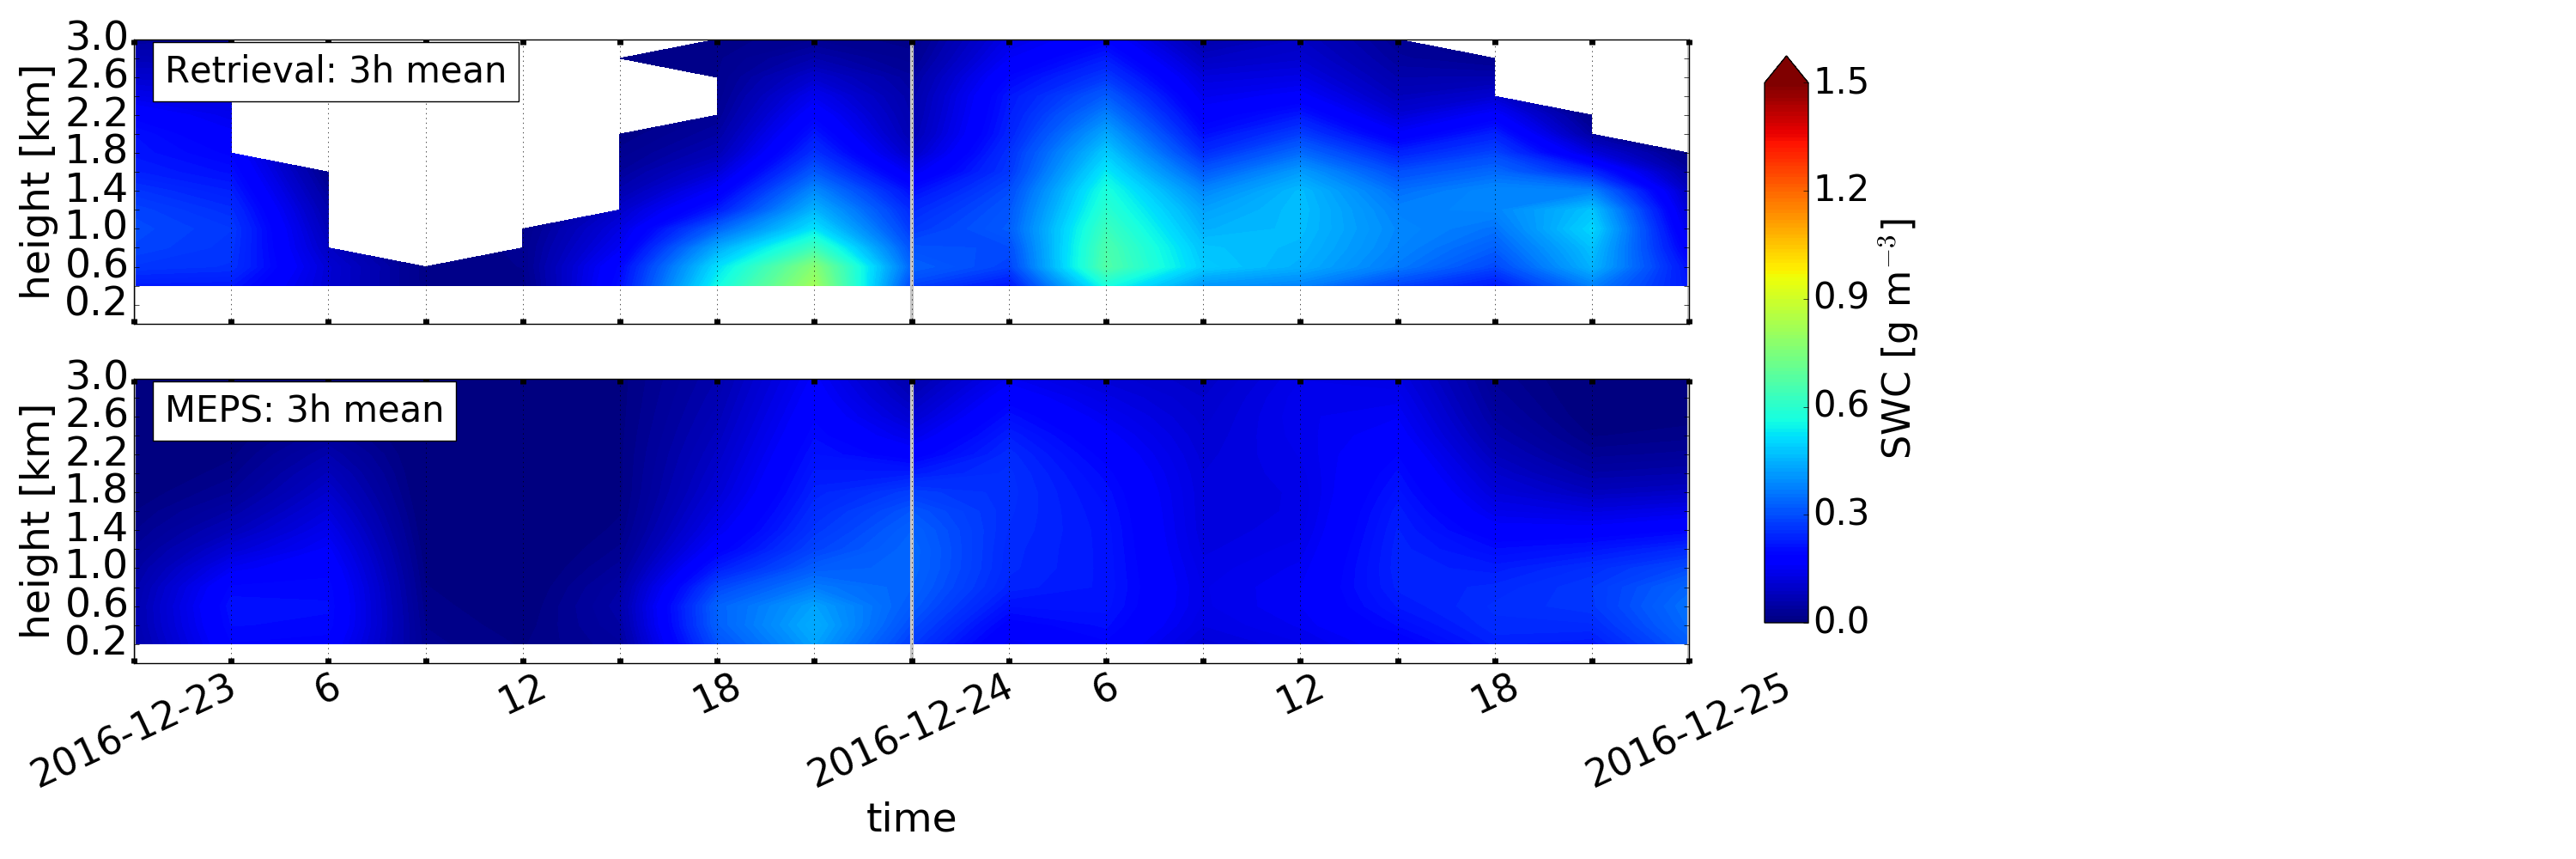
\includegraphics[trim={0.cm 0.8cm 19.cm 0.5cm},clip,width=0.9\textwidth]{./fig_vert_SWC_3h/20161223}
		\caption{}\label{fig:SWC3h:23}
	\end{subfigure}
	\caption{\textit{(Continued from previous page.)} Initialisation \SI{23}{\dec}.}
\end{figure}
%%%%%%%%% image SWC retrieval MEPS 25 %%%%%%%%%%%%%%
\begin{figure}[H]\ContinuedFloat
	\centering
	% 25/12
	\begin{subfigure}[t]{\textwidth}
		\centering
		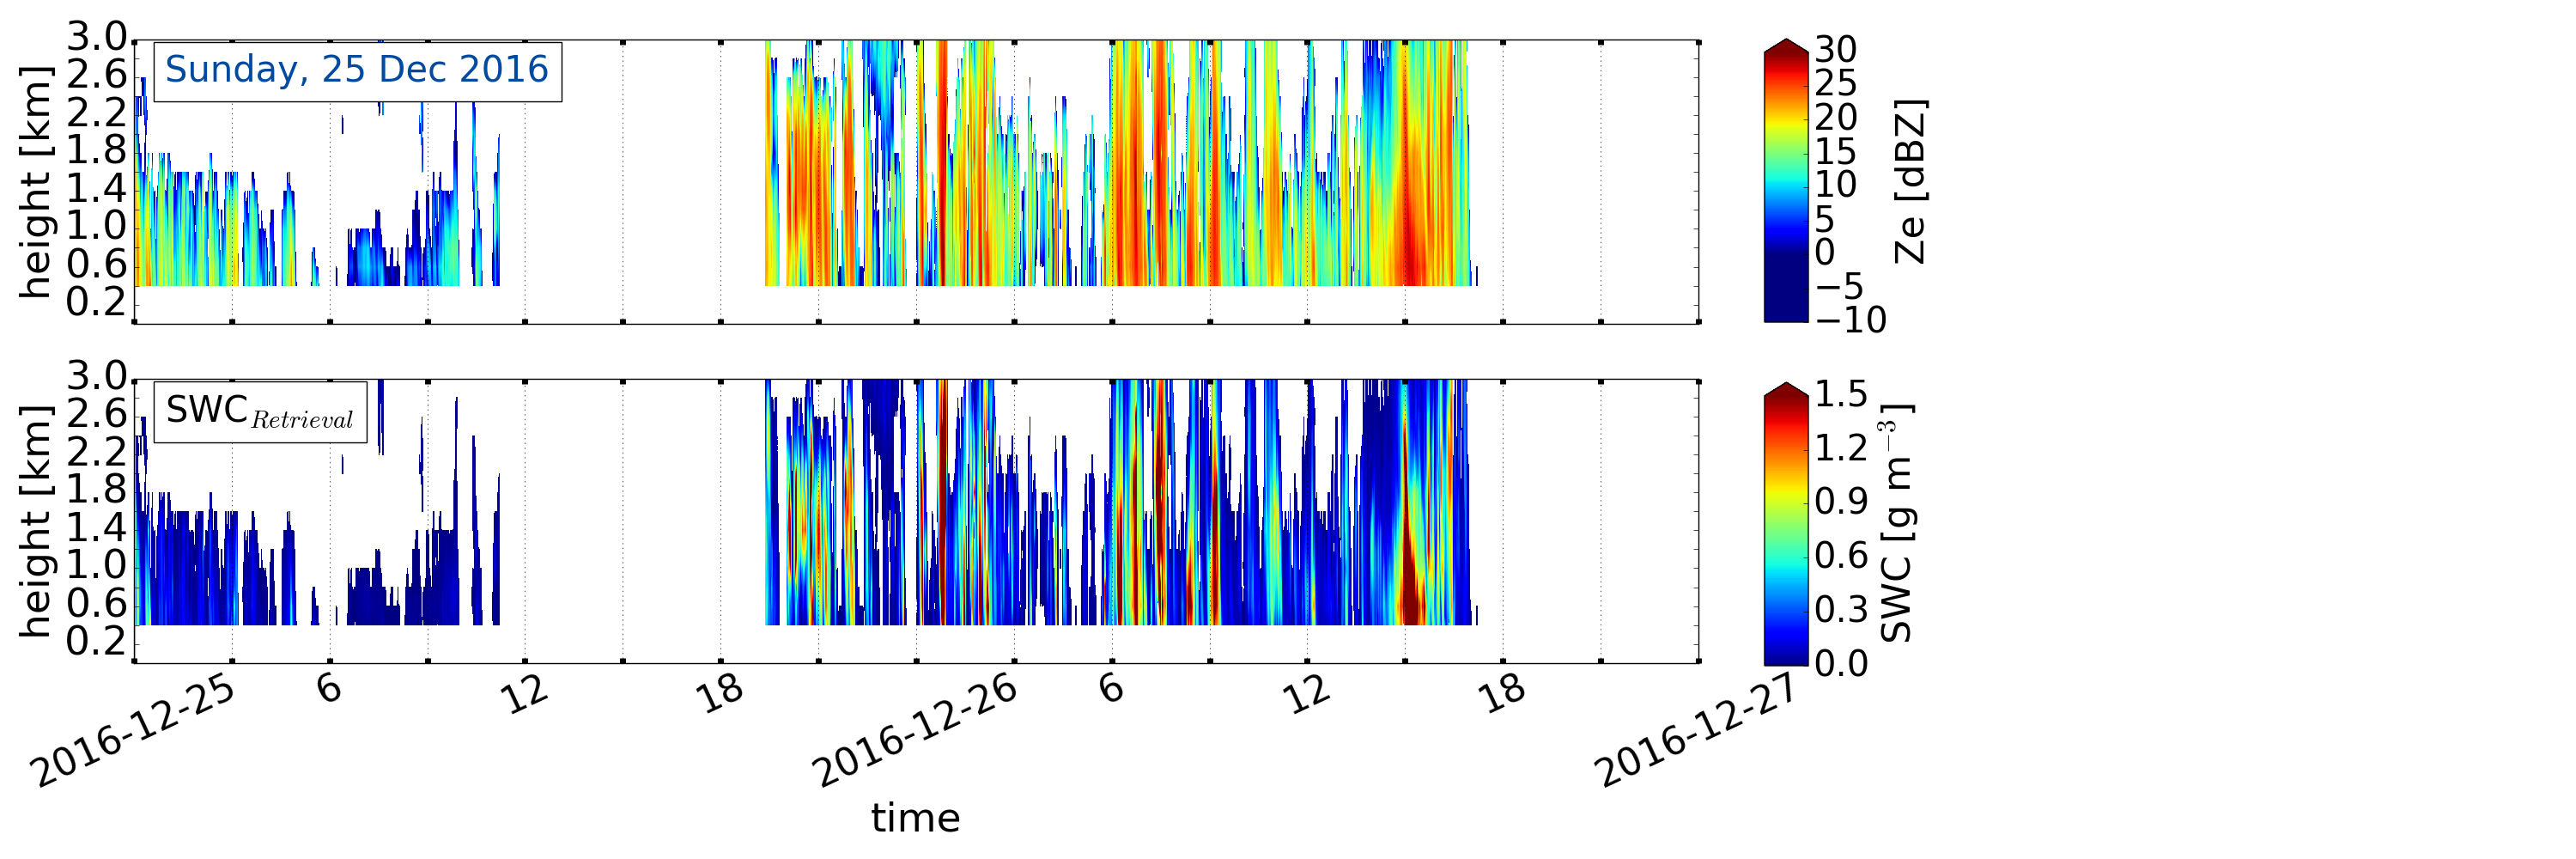
\includegraphics[trim={0.cm 2.2cm 19.cm 0.5cm},clip,width=0.9\textwidth]{./fig_obs_ret/20161225}
		\caption{}\label{fig:SWC:ret_25}
	\end{subfigure}
	% EM
	\begin{subfigure}[t]{\textwidth}
		\centering
		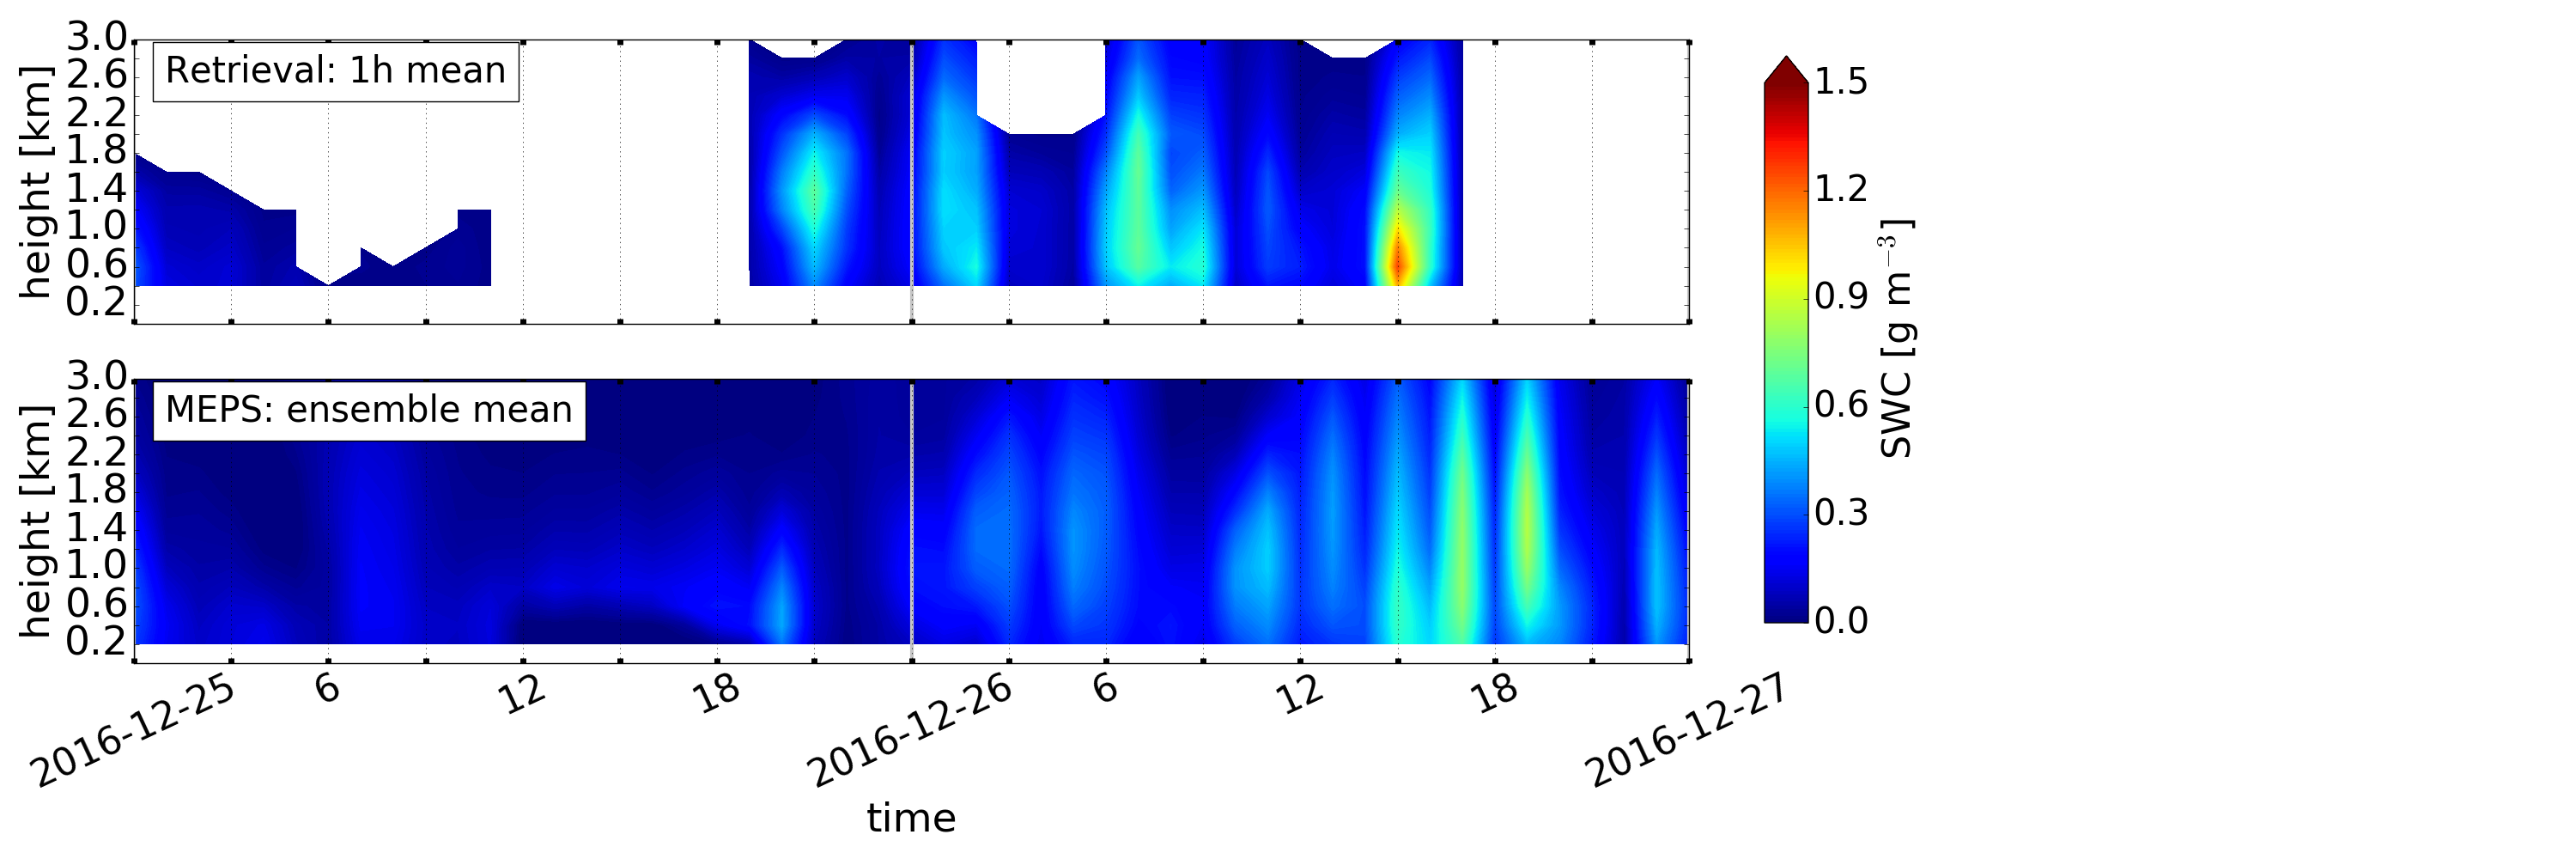
\includegraphics[trim={0.cm 2.2cm 19.cm 0.5cm},clip,width=0.9\textwidth]{./fig_vert_SWC_EM/20161225}
		\caption{}\label{fig:SWC_EM:25}
	\end{subfigure}
	% 3h
	\begin{subfigure}[t]{\textwidth}
		\centering
		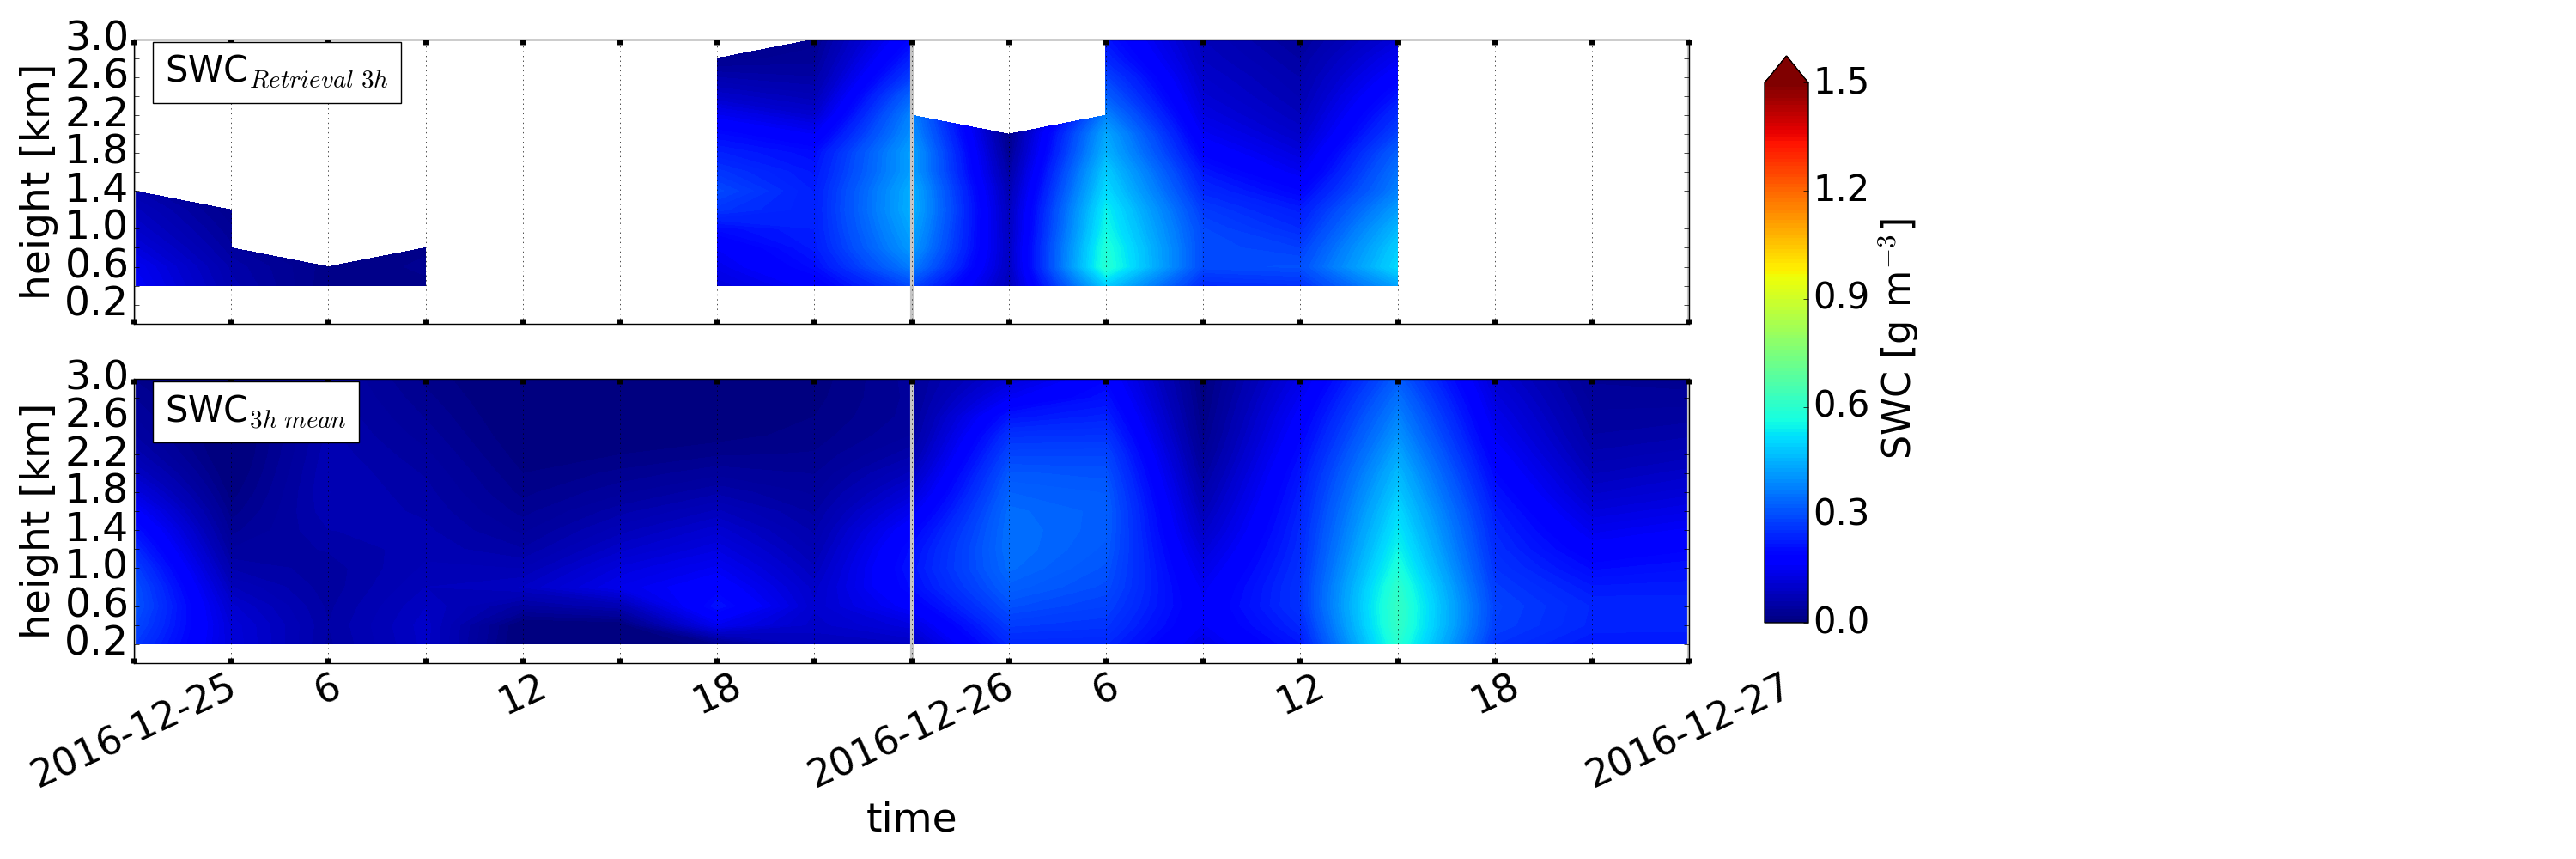
\includegraphics[trim={0.cm 0.8cm 19.cm 0.5cm},clip,width=0.9\textwidth]{./fig_vert_SWC_3h/20161225}
		\caption{}\label{fig:SWC3h:25}
	\end{subfigure}
	\caption{\textit{(Continued from previous page.)} Initialisation \SI{25}{\dec}.}
\end{figure}
%%%%%%%%% image SWC retrieval MEPS 26 %%%%%%%%%%%%%%
\begin{figure}[H]\ContinuedFloat
	\centering
	% 25/12
	\begin{subfigure}[t]{\textwidth}
		\centering
		\includegraphics[trim={0.cm 2.2cm 19.cm 0.5cm},clip,width=0.9\textwidth]{./fig_obs_ret/20161226}
		\caption{}\label{fig:SWC:ret_26}
	\end{subfigure}
	% EM
	\begin{subfigure}[t]{\textwidth}
		\centering
		\includegraphics[trim={0.cm 2.2cm 19.cm 0.5cm},clip,width=0.9\textwidth]{./fig_vert_SWC_EM/20161226}
		\caption{}\label{fig:SWC_EM:26}
	\end{subfigure}
	% 3h
	\begin{subfigure}[t]{\textwidth}
		\centering
		\includegraphics[trim={0.cm 0.8cm 19.cm 0.5cm},clip,width=0.9\textwidth]{./fig_vert_SWC_3h/20161226}
		\caption{}\label{fig:SWC3h:26}
	\end{subfigure}
	\caption{\textit{(Continued from previous page.)} Initialisation \SI{26}{\dec}.}
\end{figure}
%%%%%%%%%%%%%%%%%%%%%%%%%%%%%%%%%%%%%%%%%%%%%%%%%%%%%%%%%%%%%%%%%%%%%%%%%
\noindent
It shows also on \SI{23}{\dec} the first perturbed ensemble member does not exist and hence little snow water content is predicted for the ensemble means. 
A comparison with \SIlist{25;26}{\dec} shows the same result. Not much more snow water content is predicted when using the instantaneous values from the deterministic and first perturbed forecast (\Cref{fig:SWC1h:25}, \subref{fig:SWC1h:26}). 
\\ 
On \SI{26}{\dec} when the passage of the occlusion is predicted, the three-hourly instantaneous SWC (\Cref{fig:SWC3h:26}) as well as the average of all ensemble members (\Cref{fig:SWC_EM:26}) predict the frontal passage. 
Already initialisations \SI{39}{\hour} prior let assume that intense precipitation over a short time will occur (\Cref{fig:SWC_EM:25}, \subref{fig:SWC3h:25}). The variation of all members in \Cref{fig:EM09_25} and \subref{fig:EM09_26} indicate that almost all perturbed members would have predicted the precipitation around \SI{16}{\UTC}, but the ensemble mean weakens the result. Higher predicted values appear for deterministic forecasts than for any other ensemble member for initialisations on \SIlist{25;26}{\dec}. This bias might have led to an overestimation at the surface on \SI{26}{\dec}, where the deterministic forecast indicates higher values than the perturbed members (\Cref{fig:sfc_acc26}).  But in \Cref{fig:SWC1h:25} and \subref{fig:SWC1h:26} is the amount of snow water content very weak. 
It shows better estimations for predicted snowfall amount when using either hourly or three hourly time resolution and all ten ensemble members to create the mean than forecasts for hourly averages with only the deterministic and first perturbed member.
Still the instantaneous average values of all ensemble members are much weaker than the retrieved SWC.
\\
%%%%%%% image liquid forecast 25 %%%%%%%%%%%%%%%%
\begin{figure}[t]
	\centering
	\begin{subfigure}[b]{\textwidth}
		\centering
		\includegraphics[trim={0.cm 11.5cm 18.5cm 0.4cm},clip,width=\textwidth]{./fig_vert_LWC_EM/20161224}
		\caption{}\label{fig:LWC:24}
	\end{subfigure}
	\begin{subfigure}[b]{\textwidth}
		\centering
		\includegraphics[trim={0.cm 10cm 18.5cm 0.4cm},clip,width=\textwidth]{./fig_vert_LWC_EM/20161225}
		\caption{}\label{fig:LWC:25}
	\end{subfigure}
	\caption{200m hourly averaged LWC forecast from MEPS with all ensemble members, neglecting missing values.
		Initialised on \SIlist{24;25}{\dec} at \SI{0}{\UTC}. Liquid water content according to the colorbar.}\label{fig:LWC:2425}
\end{figure}
%%%%%%%%%%%%%%%%%%%%%%%%%%%%%%%%%%%%%%%%%%%%%%
The \SI{25}{\dec} showed patterns of liquid precipitation (\Cref{fig:res:obs_masc}) with warm temperatures (\Cref{fig:res:sfc_temp25}) and high reflectivity (\Cref{fig:ret:refl25}) between \SIrange{12}{21}{\UTC}. High reflectivity values in \Cref{fig:ret:refl25} are present around \SI{18}{\UTC} with layer thickness up to \SI{1.2}{\km}. 
To see if liquid precipitation was predicted, the atmospheric cloud condensed water content and rainfall amount in model levels is summed. \Cref{fig:LWC:24} and \subref{fig:LWC:25} show liquid water content for initialisations at either \SI{24}{\dec} or \SI{25}{\dec}. 
Positive surface temperatures were forecasted between \SIrange{12}{21}{\UTC} (\Cref{fig:res:sfc_temp25}). Initialisations more than \SI{24}{\hour} prior show already the occurrence of the liquid layer. \Cref{fig:LWC:24} or \subref{fig:LWC:25} show also a narrow thickness up to \SI{800}{\metre}. 
In Norwegian mountainous terrain is this an important feature since precipitation change can lead to a high risk for people. The avalanche danger increases with the precipitation change especially during high wind speeds. Since MEPS forecasts the liquid layer correctly in depth and length it seems to be a good interaction between the surface model and the vertical prediction. 
This follows a high accuracy of the forecasting system and the advantage of using a high resolution convective scheme model.
\\
\\
%%% table verification %%%%%%%%%%%%%%%%%%%%%%%%%%%%%%%%%%%%%
\begin{table}[t!]
	\begin{center}
		\caption{Interpretation of the coefficient of variation for SWC.} \label{tab:verification}
		\begin{tabular}{lc|c}
			\hline\hline
			\multicolumn{2}{c|}{\textbf{Size of CV}} & {\textbf{Interpretation}} \\ 
			\multicolumn{2}{c|}{[\SI{}{\percent}]} & variability \\ \hline \hline 
			\multicolumn{2}{c|}{\numrange{0}{< 25}} & negligible  \\ \hline
			\multicolumn{2}{c|}{\numrange{25}{< 50}} & low \\ \hline
			\multicolumn{2}{c|}{\numrange{50}{< 75}} & moderate \\ \hline
			\multicolumn{2}{c|}{\numrange{75}{< 100}} & high \\ \hline
			\multicolumn{2}{c|}{\num{100} to $\infty$} & very high  \\ \hline \hline
		\end{tabular}
	\end{center}
\end{table}
%%%%%%%%%%%%%%%%%%%%%%%%%%%%%%%%%%%%%%%%%%%%%%%%%%%%%%%%%%%%%%%%%%%%%%%%%
\noindent
%A validation of how well the forecast performed is difficult to do at this state, since the time resolution of MEPS is coarse compared to the observations. 
For the first glance operates the forecast well when compared to vertical observations. One possibility is to assess the variability of all ensemble member with the coefficient of variation described in \Cref{sec:ens_mean_spread}. 
\Cref{fig:vari:EM22,fig:vari:EM25,fig:vari:EM26} show the coefficient of variation for SWC, which is the standard deviation of the ten ensemble members divided by the mean of all ensemble members. This coefficient gives the possibility to compare the SWC results for different days with different values. It follows for even a low ensemble spread of SWC (standard deviation of all ensemble members) then the different members do not need to be less variable.
\\
The grey line in \Cref{fig:ens_vari} shows the ensemble mean of the hourly predicted SWC values. The darker the colour in \Cref{fig:ens_vari} the smaller is the variation of the SWC relative to the mean. Initialisations on \SI{23}{\dec} does not exist, because it had too few ensemble members (only six) to create a reasonable verification. Therefore, the initialsation on \SI{22}{\dec} is used. The interpretation of the coefficient of variation for SWC is presented in \Cref{tab:verification}.
%%%%%%% image variability %%%%%%%%%%%%%%%%
\begin{figure}[t!]
	\centering
	\begin{subfigure}[b]{\textwidth}
		\includegraphics[trim={0cm 5cm 0cm 0cm},clip,width=\textwidth]{./fig_variation/20161222}
		\caption{}\label{fig:vari:EM22}
	\end{subfigure}
	\begin{subfigure}[b]{\textwidth}
		\includegraphics[trim={0cm 5cm 0cm 0cm},clip,width=\textwidth]{./fig_variation/20161225}
		\caption{}\label{fig:vari:EM25}
	\end{subfigure}
	\begin{subfigure}[b]{\textwidth}
		\includegraphics[trim={0cm 0cm 0cm 0cm},clip,width=\textwidth]{./fig_variation/20161226}
		\caption{}\label{fig:vari:EM26}
	\end{subfigure}
	\caption{SWC variation of the ten ensemble members of MEPS. The lighter the colour according to the colourbar the higher the variation between the perturbed ensemble members. In grey the ensemble mean of all ten members.}\label{fig:ens_vari}
\end{figure}
%%%%%%%%%%%%%%%%%%%%%%%%%%%%%%%%%%%%%%%%%%%%%%
\noindent
The CV agrees well with the prediction of the occlusion on \SI{23}{\dec} after \SI{15}{\UTC}. The variability between the members is small and show a good agreement on the occurrence of snow precipitation. \Cref{fig:EM09_22,fig:EM0923} show the same variability, where all ensemble member agree on the passage after \SI{16}{\UTC}. While comparing only six ensemble members in \Cref{fig:EM09_23}, one could assume that the uncertainty of all ensemble members during the up-slope storm is low, but not as certain as for an initialisation on \SI{22}{\dec} at \SI{0}{\UTC}.
\\
A larger difference between the ensemble members is shown for the passage of the occlusion on \SI{26}{\dec}. Initialisations on \SI{25}{\dec} present a lower variability for the passage after \SI{15}{\UTC} on \SI{26}{\dec} than initialisations less than \SI{24}{\hour} prior. Therefore, an increase of variability after shorter time and an increase in uncertainty. Again, this is not a fair comparison since hourly instantaneous values are used and there might be a time delay of half an hour about the passage which would follow it is not seen in the model forecast. 
\\
Another way to see how the MEPS forecast performed compared to the vertical observations can be done by correlating the observed SWP with the ensemble member snow water content.
% %%% fig correlation %%%%%%%%%%%%%%%%%%%%%%%%%%%%%%%%%%%%%
% \begin{figure}[t!]
% 	\centering
%     \begin{subfigure}[b]{0.49\textwidth}
%     	\includegraphics[width=\textwidth]{./fig_SWP_scat/20161222}
%         \caption{}\label{fig:scatSWP:22}
%     \end{subfigure}
%     \begin{subfigure}[b]{0.49\textwidth}
%     	\includegraphics[width=\textwidth]{./fig_SWP_scat/20161223}
%         \caption{}\label{fig:scatSWP:23}
%     \end{subfigure}
%     \begin{subfigure}[b]{0.49\textwidth}
%     	\includegraphics[width=\textwidth]{./fig_SWP_scat/20161225}
%         \caption{}\label{fig:scatSWP:25}
%     \end{subfigure}
%     \begin{subfigure}[b]{0.49\textwidth}
%     	\includegraphics[width=\textwidth]{./fig_SWP_scat/20161226}
%         \caption{}\label{fig:scatSWP:26}
%     \end{subfigure}
%     \caption{}\label{fig:scatSWP}
% \end{figure}
% %%%%%%%%%%%%%%%%%%%%%%%%%%%%%%%%%%%%%%%%%%%%%%%%%%%%%%%%%%%%%%%%%%%%%%%%%
\\
\\
One question to answer in this work is if the operational model MEPS gets large scale features correctly. As discussed here and in \Cref{sec:res:large_scale_sfc} it seems that the model is able to cover the development of large scale features and its associated precipitation. Even with the intensification of the storm seems MEPS to be able to predict extreme events such as the Christmas event, but might have some issues predicting fast transitions of frontal boundaries. 
\\
MEPS is also able to distinguish between liquid and solid precipitation in layer thickness and duration for time resolution of one hour. This can be a major advantage since a change in temperature and associated precipitation transformation can lead to high safety issues in the Norwegian mountains, especially during winter. With the knowledge more than \SI{24}{\hour} prior can risk notice be send out to the population and rescue teams can prepare in advance. Furthermore, roads and train tracks can be closed to increase the safety of people.
%\\
\textcolor{red}{I'm not sure if the above mentioned should be here?! }
%%%%%%%%%%%%%%%%%%%%%%%%%%%%%%%%%%%%%%%%%%%%%%%%%%%%%%%%%%%%%%%%%%%%%%%%%%
%%%%%%%%% surface overestimation - vertical? %%%%%%%%%%%%%%
%\section{Surface overestimation and the vertical}

%%%%%%%%% Local affects %%%%%%%%%%%%%%
\section{Orographic influence on precipitation}\label{sec:res:oro_infl}
The Haukeliseter is suspended to high wind speeds during the winter. The previous results have shown, that wind plays an important role on the precipitation. The mountain plateau is surrounded by higher mountains to the west and more open to the south east \citep{wolff_measurements_2013,wolff_derivation_2015}, this orography seems to influence the vertical precipitation pattern. The correlation between wind speed observations and forecast have shown an overestimation of predicted wind speed throughout the event (\Cref{fig:scat:ws2123} and \subref{fig:scat:ws2426}). \citet{muller_arome-metcoop:_2017} already mentioned the weakness of too strong wind prediction in AROME-MetCoOp.
\\
On \SIlist{21;23}{\dec} wind directions from the south-east and south were observed, respectively. As earlier discussed in \Cref{sec:res:large_scale_sfc} and \subref{sec:res:large_scale_vert} was the wind change associated with the occlusion passage on \SI{23}{\dec}. The wind direction on \SI{21}{\dec} change was also related to the large scale synoptic flow but was not associated with a frontal passage. A comparison with the large scale weather analysis from ECMWF shows, that the large scale surface wind is from the south-west at \SI{6}{\UTC} on \SI{21}{\dec} (\Cref{fig:GP21_06}) and has changed to west at \SI{12}{\UTC} (\Cref{fig:GP21_12}). The observations at the Haukeliseter site show between \SIrange{6}{12}{\UTC} wind from south-east, while the predicted wind direction is from south in \Cref{fig:res:sfc_wd21}. The local wind direction influenced the precipitation pattern in the vertical in the matter that a more consistent storm structure was observed and predicted between \SIrange{9}{12} {\UTC} (\Cref{fig:SWC:ret_21,fig:SWC_EM:21,fig:SWC3h:21}). 
%%%%%%%%% image SWC retrieval MEPS 21 %%%%%%%%%%%%%%
\begin{figure}[ht!]
	\centering
	% 21/12
	\begin{subfigure}[t]{\textwidth}
		\centering
		\includegraphics[trim={0.cm 2.2cm 19.cm 0.5cm},clip,width=0.9\textwidth]{./fig_obs_ret/20161221}
		\caption{}\label{fig:SWC:ret_21}
	\end{subfigure}
	% EM
	\begin{subfigure}[t]{\textwidth}
		\centering
		\includegraphics[trim={0.cm 2.2cm 19.cm 0.5cm},clip,width=0.9\textwidth]{./fig_vert_SWC_EM/20161221}
		\caption{}\label{fig:SWC_EM:21}
	\end{subfigure}
	% 3h
	\begin{subfigure}[t]{\textwidth}
		\centering
		\includegraphics[trim={0.cm 0.8cm 19.cm 0.5cm},clip,width=0.9\textwidth]{./fig_vert_SWC_3h/20161221}
		\caption{}\label{fig:SWC3h:21}
	\end{subfigure}
	\caption{Initialisation \SI{21}{\dec} \SI{0}{\UTC}. 
		(\protect\subref{fig:SWC:ret_21},\protect\subref{fig:SWC:ret_24}) Upper panel: MRR reflectivity for \SI{48}{\hour}, lower panel minutely retrieved SWC. 
		(\protect\subref{fig:SWC_EM:21}, \protect\subref{fig:SWC_EM:24}) Upper panel: hourly averaged retrieved SWC, lower panel instantaneous hourly averaged forecast of all ensemble member SWC, neglecting missing values. 
		(\protect\subref{fig:SWC3h:21}, \protect\subref{fig:SWC3h:24}) Upper panel three hourly averaged retrieved SWC, lower panel instantaneous three hourly averaged forecast of all ensemble member SWC.   }\label{fig:ret:SWC21_24}
\end{figure}
%%%%%%%%%%%%%%%%%%%%%%%%%%%%%%%%%%%%%%%%%%%%%%
\noindent
Both days show a more consistent storm structure with not as intense snow water content than for storm patterns from the west. 
\Cref{fig:site:kartverket} presents the local topography around Haukeliseter and \Cref{fig:meps:site} shows the topography resolved by MEPS. It shows that MEPS is able to cover some of the complex structure around the site, with the higher mountain to the west and the valley to the south-east. The prediction model seems to forecast the wind direction overall well, only on \SI{21}{\dec} before \SI{10}{\UTC} is a south instead of a south-east wind predicted. It displays that even if the large scale wind is from the south-west is the local wind rather from the south or south-east. The orography in \Cref{fig:site:kartverket} lets assume that large scale south-west wind is forced along the valley laying in south-east direction. As \Cref{fig:SWC_EM:21} indicates is the model obviously able to cover almost the exact timing of the up-slope storm pattern. The variability of each ensemble member is again presented in \Cref{fig:EM09_21}. It shows that almost all ensemble member agree on the occurrence of the storm pattern during \SIrange{9}{12}{\UTC}.
\\
Wind from the west and therefore over mountains followed always a pulsing with more intense precipitation in the vertical (\Cref{fig:ret:SWC} and \ref{fig:ret:SWC2}). This effect might be related to wave breaking at the mountain and result into a pulsing precipitation pattern. More precipitation events need to be studied to understand this effect around the Haukeliseter site. MEPS seems not to cover all pulses during the course of a day, which is related to the time resolution of the forecast values. Since the prediction values exist only every hour the model might miss some of the high pulses \SI{30}{\minute} before or after the occurrence. 
\\
One outcome of the presented study is that MEPS is able to resolve the local topography and predicts the wind direction in almost all the cases correctly. It did not cover the south-east wind direction on \SI{21}{\dec}, which must be related to the local topography. It seems more intuitive for the model to force large scale south-westerly flow into south direction. As seen in \Cref{fig:meps:site} must the wind go along the \SI{7.2}{\degree} longitude, since a higher elevation is to the west and a \SI{1350}{\metre} high mountain to the east. This true prediction of wind direction leads then to the correct estimation of vertical precipitation patterns. 
%%%%%%%%% image SWC retrieval MEPS 24 %%%%%%%%%%%%%%
\begin{figure}[ht!]\ContinuedFloat
	\centering
	% 24/12
	\begin{subfigure}[t]{\textwidth}
		\centering
		\includegraphics[trim={0.cm 2.2cm 19.cm 0.5cm},clip,width=0.9\textwidth]{./fig_obs_ret/20161224}
		\caption{}\label{fig:SWC:ret_24}
	\end{subfigure}
	% EM
	\begin{subfigure}[t]{\textwidth}
		\centering
		\includegraphics[trim={0.cm 2.2cm 19.cm 0.5cm},clip,width=0.9\textwidth]{./fig_vert_SWC_EM/20161224}
		\caption{}\label{fig:SWC_EM:24}
	\end{subfigure}
	% 3h
	\begin{subfigure}[t]{\textwidth}
		\centering
		\includegraphics[trim={0.cm 0.8cm 19.cm 0.5cm},clip,width=0.9\textwidth]{./fig_vert_SWC_3h/20161224}
		\caption{}\label{fig:SWC3h:24}
	\end{subfigure}
	\caption{\textit{(Continued from previous page.)} Initialisation \SI{26}{\dec}.}
\end{figure}
%%%%%%%%%%%%%%%%%%%%%%%%%%%%%%%%%%%%%%%%%%%%%%
\noindent
\Cref{sec:sfc_acc} describes the overestimation of surface snow accumulation during the intensification of the extreme storm. MEPS forecasted more ground accumulation than it was observed. One approach was to see, if the wind might have had an influence on the surface measurement of the double fence, which did not show to be true. A comparison of the hourly values of MEPS, shows that neither on \SI{24}{\dec} nor on \SI{25}{\dec} or \SI{26}{\dec} the vertical snow amount was higher than the observations (\Cref{fig:SWC_EM:24}, \ref{fig:SWC_EM:25}, and \subref{fig:SWC_EM:26}). \Cref{fig:EM09} shows very intense individual ensemble members, but no prominent sign of overestimation when the surface miscalculation was present. 
\\
During \SIrange{24}{26}{\dec} was the wind constantly from the west with higher wind speeds observed than during \SIrange{21}{23}{\dec} (\Cref{fig:res:sfc_wd23}, \subref{fig:res:sfc_wd25}, \subref{fig:res:sfc_wd26}; \Cref{fig:res:sfc_wd21}, \subref{fig:res:sfc_wd22}, \subref{fig:res:sfc_wd24}; \Cref{fig:res:sfc_ws23}, \subref{fig:res:sfc_ws25}, \subref{fig:res:sfc_ws26}, and \Cref{fig:res:sfc_ws21}, \subref{fig:res:sfc_ws22}, \subref{fig:res:sfc_ws24}). \Cref{fig:scat:wd2123} and \subref{fig:scat:wd2426} indicate a better agreement between the forecasted and observed wind directions when precipiation overestimation occurred. During \SIrange{24}{26}{\dec} were the observed wind speeds higher than on the previous days, and as \Cref{fig:scat:ws2123} and \subref{fig:scat:ws2426} present is the correlation between observation and forecasts lower during high wind speeds. The high wind speeds from the west followed a pulsing storm pattern with intense and less intense precipitation. The pulsing pattern is forecasted by MEPS for initialisations longer than \SI{24}{\hour} prior. Since the model gets the wind direction correctly and the affect of local mountains it follows that there seems to be some kind of interaction issue between the vertical snow amount and the surface accumulation. Vertical instantaneous values every hour can lead to a misinterpretation of the here presented results. 
%%%%%%% image variability %%%%%%%%%%%%%%%%
\begin{figure}[t!]
	\centering
	\begin{subfigure}[b]{\textwidth}
		\includegraphics[trim={0cm 0cm 0cm 0cm},clip,width=\textwidth]{./fig_variation/20161224}
		\caption{}\label{fig:vari:EM24}
	\end{subfigure}
	\caption{SWC variation of the ten ensemble members of MEPS. The lighter the colour according to the colourbar the higher the variation between the perturbed ensemble members. In grey the ensemble mean of all ten members.}\label{fig:ens_vari24}
\end{figure}
%%%%%%%%%%%%%%%%%%%%%%%%%%%%%%%%%%%%%%%%%%%%%%
The ensemble variability in \Cref{fig:vari:EM24}, \Cref{fig:vari:EM25}, and \subref{fig:vari:EM26} show that the ensemble members are divided about the existence of the exact pulsing. 
\\
\\
While the wind direction of MEPS has a good agreement shows the wind speed larger values over all days. Although MEPS includes ten perturbed ensemble members the insufficiency of AROME-MetCoOp too high wind prediction in extreme situations is not resolved. The regional model wind prediction is still dependent on the intensity of the storm. As \cite{muller_arome-metcoop:_2017} also mentioned are higher wind speeds in general better forecasted in AROME-MetCoOp than in ECMWF. 
%%%%%%%%%%%%%%%%%%%%%%%%%%%%%%%%%%%%%%%%%%%%%%%%%%%%%%%%%%%%%%%%%%%%%%%%%%
\section{Discussion all}
\textcolor{red}{This section needs another title! Just collecting up-coming disscussion points}
Of course, more storms should be investigated to find the exact correlation between the surface observations and the estimated accumulation to see if the deviation keeps as small for different snow patterns at Haukeliseter. 

%%%%%%%%%%%%%%%%%%%%%%%%%%%%%%%%%%%%%%%%%%%%%%%%%%%%%%%%%%%%%%%%%%%%%%%%%



%
%%%%%%%%%%%%%%%%%%%%%%%%%%%%%%%%%%%%%%%%%%%%%%%%%%%%%%%%%%%%%%%%%%%%%%%%%%%
%%%%%%%%%% SWC COMPARISON %%%%%%%%%%%%%%
%% !TeX spellcheck = en_GB
\section{SWC and SWP from MEPS and the optimal estimation retrieval}
Images for the liquid water content evaluated in MEPS can be found in \Cref{app:LWP_MEPS}. 

%%% table SWP and LWP max %%%%%%%%%%%%%%%%%%%%%%%%%%%%%%%%%%%%%
% !TeX spellcheck = en_GB
\begin{table}[h!]
	\begin{center}
		\caption{Maximum values of the snow water and liquid water content from the retrieval and MEPS}\label{tab:max_val}
		\begin{tabular}{ll|c|c|c|c|c|c} 
			\hline \hline
			& & \textbf{SWC}  & \textbf{HEIGHT}  & \textbf{TIME} & \textbf{LWC}  & \textbf{HEIGHT}  & \textbf{TIME}  \\
			& & [\SI{}{\kg\per\cubic\meter}] & [\SI{}{\meter}] &  & [\SI{}{\kg\per\cubic\meter}] & [\SI{}{\meter}] &   \\
			\hline \hline
			\multicolumn{8}{c}{\textbf{Wed, 21 Dec 2016}} \\ \hline
			\multicolumn{2}{l|}{RETRIEVAL} & 1.08 & 600.0 & \SI{16}{\UTC} & & & \\
			\multicolumn{2}{l|}{MEPS} &  &  & & & & \\
			& ensemble mean & \num{1.24} & \num{1400.0} & \SI{20}{\UTC} & & & \\
			& control & \num{2.11} & \num{1400.0} & \SI{20}{\UTC} & \num{0.15} & \num{2200.0} & \SI{23}{\UTC}\\ \hline \hline
			\multicolumn{8}{c}{\textbf{Thu, 22 Dec 2016}} \\ \hline
			\multicolumn{2}{l|}{RETRIEVAL} & \num{1.46} & \num{1200.0} & \SI{10}{\UTC} & & & \\
			\multicolumn{2}{l|}{MEPS} &  &  & & & & \\
			& ensemble mean & \num{1.54} & \num{2200.0} & \SI{14}{\UTC} & & & \\
			& control & \num{1.35} & \num{1400.0} & \SI{12}{\UTC} & \num{0.20} & \num{2000.0} & 0\SI{02}{\UTC} \\ \hline \hline
			\multicolumn{8}{c}{\textbf{Fri, 23 Dec 2016}} \\ \hline
			\multicolumn{2}{l|}{RETRIEVAL} & \num{0.91} & \num{600.0} & \SI{23}{\UTC} & & & \\
			\multicolumn{2}{l|}{MEPS} &  &  & & & & \\
			& ensembel mean & \num{0.54} & \num{400.0} & \SI{20}{\UTC} & & & \\
			& control & \num{0.54} & \num{400.0} & \SI{20}{\UTC} & \num{0.14} & \num{1000.0} & \SI{15}{\UTC} \\ \hline \hline
			\multicolumn{8}{c}{\textbf{Sat, 24 Dec 2016}} \\ \hline
			\multicolumn{2}{l|}{RETRIEVAL} & \num{1.39} & \num{1000.0} & 0\SI{06}{\UTC} & & & \\
			\multicolumn{2}{l|}{MEPS} &  &  & & & & \\
			& ensembel mean & \num{0.70} & \num{1400.0} & 0\SI{07}{\UTC} & & & \\
			& control & \num{0.73} & \num{1400.0} & \SI{17}{\UTC} & \num{0.33} & \num{1200.0} & 0\SI{09}{\UTC} \\ \hline \hline
			\multicolumn{8}{c}{\textbf{Sun, 25 Dec 2016}} \\ \hline
			\multicolumn{2}{l|}{RETRIEVAL} & \num{0.69} & \num{1400.0} & \SI{21}{\UTC} & & & \\
			& ensembel mean & \num{0.44} & \num{400.0} & \SI{20}{\UTC} & & & \\
			& control & \num{0.50} & \num{800.0} & \SI{20}{\UTC} & \num{0.34} & \num{200.0} & \SI{17}{\UTC} \\ \hline \hline
			\multicolumn{8}{c}{\textbf{Mon, 26 Dec 2016}} \\ \hline
			\multicolumn{2}{l|}{RETRIEVAL} & \num{1.25} & \num{600.0} & \SI{15}{\UTC} & & & \\
			& ensembel mean & \num{0.95} & \num{800.0} & \SI{16}{\UTC} & & & \\
			& control & \num{1.55} & \num{1000.0} & \SI{11}{\UTC} & \num{0.17} & \num{2400.0} & 0\SI{09}{\UTC} \\ \hline \hline
			\multicolumn{8}{c}{\textbf{Tue, 27 Dec 2016}} \\ \hline
			\multicolumn{2}{l|}{RETRIEVAL} & -- & -- & -- & & & \\
			& ensembel mean & \num{0.16} & \num{400.0} & 0\SI{00}{\UTC} & & & \\
			& control & \num{0.16} & \num{400.0} & 0\SI{00}{\UTC} & \num{0.25} & \num{800.0} & \SI{23}{\UTC} \\ \hline \hline
		\end{tabular}
	\end{center}
\end{table}
%%%%%%%%%%%%%%%%%%%%%%%%%%%%%%%%%%%%%%%%%%%%%%%%%%%%%%%%%%%%%%%%%%%%%%%%%%

%%% image SWC, SWP Retrieval MEPS comparison %%%%%%%%%%%%%%%%%%%%%%%%%%%%%%%%%%%%%
% !TeX spellcheck = en_GB
%\begin{landscape}
\begin{figure}[h]
	\centering
    	% 21/12
		\begin{subfigure}[b]{0.8\textwidth}
			\includegraphics[trim={0.5cm 0.5cm 17.5cm .5cm},clip,width=\textwidth]{./fig_SWC/20161221}
			\caption{Wednesday, \SI{21}{\dec}}\label{fig:SWC21}
		\end{subfigure}
\end{figure}
\begin{figure}\ContinuedFloat
   	\centering
		% 22/12
	\begin{subfigure}[b]{0.8\textwidth}
			\includegraphics[trim={0.5cm 0.5cm 17.5cm .5cm},clip,width=\textwidth]{./fig_SWC/20161222}
			\caption{Thursday, \SI{22}{\dec}}\label{fig:SWC22}
		\end{subfigure}
	\end{figure}
    \begin{figure}\ContinuedFloat
   		\centering
		% 23/12
		\begin{subfigure}[b]{0.8\textwidth}
			\includegraphics[trim={0.5cm 0.5cm 17.5cm .5cm},clip,width=\textwidth]{./fig_SWC/20161223}
			\caption{Friday, \SI{23}{\dec}}\label{fig:SWC23}
		\end{subfigure}
	\end{figure}
    \begin{figure}\ContinuedFloat
   		\centering
		% 24/12
		\begin{subfigure}[b]{0.8\textwidth}
			\includegraphics[trim={0.5cm 0.5cm 17.5cm .5cm},clip,width=\textwidth]{./fig_SWC/20161224}
			\caption{Saturday, \SI{24}{\dec}}\label{fig:SWC24}
		\end{subfigure}
	\end{figure}
    \begin{figure}\ContinuedFloat
   		\centering
		% 25/12
		\begin{subfigure}[b]{0.8\textwidth}
			\includegraphics[trim={0.5cm 0.5cm 17.5cm .5cm},clip,width=\textwidth]{./fig_SWC/20161225}
			\caption{Sunday, \SI{25}{\dec}}\label{fig:SWC25}
		\end{subfigure}
	\end{figure}
    \begin{figure}\ContinuedFloat
   		\centering
		% 26/12
		\begin{subfigure}[b]{0.8\textwidth}
			\includegraphics[trim={0.5cm 0.5cm 17.5cm .5cm},clip,width=\textwidth]{./fig_SWC/20161226}
			\caption{Monday, \SI{26}{\dec}}\label{fig:SWC26}
		\end{subfigure}
        \caption{Upper panel: MRR reflectivity in \SI{}{\dB Z}. 2nd panel: SWC optimal estimation retrieval output every second in \SI{}{\gram\per\cubic\metre}. 3rd panel: hourly-averaged SWC optimal estimation retrieval output. 4th panel: \SI{200}{\metre}-averaged SWC deterministic forecast from MEPS. Lowest panel: SWP from MEPS, initialised at \SI{00}{\UTC}. Black line represents the deterministic forecast and the grey lines the nine perturbed members. In blue the SWP from the averaged retrieval output.}\label{fig:SWC}
	\end{figure}
	

%%%%%%%%%%%%%%%%%%%%%%%%%%%%%%%%%%%%%%%%%%%%%%%%%%%%%%%%%%%%%%%%%%%%%%%%%%




%%%%%%%%%%%%%%%%%%%%%%%%%%%%%%%%%%%%%%%%%%%%%%%%%%%%%%%%%%%%%%%%%%%%%%%%%%%
%
%%\newpage
%%%%%%%%%%%%%%%%%%%%%%%%%%%%%%%%%%%%%%%%%%%%%%%%%%%%%%%%%%%%%%%%%%%%%%%%%%%
%%%%%%%%%% ensemble verification %%%%%%%%%%%%%%
%% !TeX spellcheck = en_GB
\subsection{Verification of MEPS ensemble members}\label{sec:variation}
%%%%%%%%% image SWC retrieved %%%%%%%%%%%%%%
% !TeX spellcheck = en_GB

%%%%%%%
\begin{figure}[t]
	\centering
    % 20/12
		\begin{subfigure}[t]{\textwidth}		\includegraphics[trim={0.cm 5.3cm 0cm 0cm},clip,width=\textwidth]{./fig_variation/20161220}
			\caption{}\label{fig:ens_vari20}
		\end{subfigure}
%\end{figure}
%\begin{figure}\ContinuedFloat
    % 21/12
		\begin{subfigure}[t]{\textwidth}		\includegraphics[trim={0.cm 5.3cm 0cm 0cm},clip,width=\textwidth]{./fig_variation/20161221}
			\caption{}\label{fig:ens_vari21}
		\end{subfigure}
       
       % colourbar
     	\begin{subfigure}[t]{\textwidth}		\includegraphics[trim={15.cm 0cm 15cm 21cm},clip,width=\textwidth]{./fig_variation/20161224}
		\end{subfigure}
\end{figure}
\begin{figure}[t]\ContinuedFloat
    % 22/12
		\begin{subfigure}[t]{\textwidth}		\includegraphics[trim={0.cm 5.3cm 0cm 0cm},clip,width=\textwidth]{./fig_variation/20161222}
			\caption{}\label{fig:ens_vari22}
		\end{subfigure}
    % 23/12
% 		\begin{subfigure}[t]{\textwidth}		\includegraphics[trim={0.cm 0cm 0cm 0cm},clip,width=\textwidth]{./fig_variation/20161223}
% 			\caption{}\label{fig:ens_vari23}
% 		\end{subfigure}
    % 24/12
		\begin{subfigure}[t]{\textwidth}		\includegraphics[trim={0.cm 5.3cm 0cm 0cm},clip,width=\textwidth]{./fig_variation/20161224}
			\caption{}\label{fig:ens_vari24}
		\end{subfigure}
        
     % colourbar
     	\begin{subfigure}[t]{\textwidth}		\includegraphics[trim={15.cm 0cm 15cm 21cm},clip,width=\textwidth]{./fig_variation/20161224}
		\end{subfigure}
\end{figure}
\begin{figure}[t]\ContinuedFloat
	\centering
    % 25/12
		\begin{subfigure}[t]{\textwidth}		\includegraphics[trim={0.cm 5.3cm 0cm 0cm},clip,width=\textwidth]{./fig_variation/20161225}
			\caption{}\label{fig:ens_vari25}
		\end{subfigure}
    % 26/12
		\begin{subfigure}[t]{\textwidth}		\includegraphics[trim={0.cm 5.3cm 0cm 0cm},clip,width=\textwidth]{./fig_variation/20161226}
			\caption{}\label{fig:ens_vari26}
		\end{subfigure}
%     % 27/12
% 		\begin{subfigure}[t]{\textwidth}		\includegraphics[trim={0.cm 5.3cm 0cm 0cm},clip,width=\textwidth]{./fig_variation/20161227}
% 			\caption{}\label{fig:ens_spread27}
% 		\end{subfigure}
        
    % colourbar
     	\begin{subfigure}[t]{\textwidth}		\includegraphics[trim={15.cm 0cm 15cm 21cm},clip,width=\textwidth]{./fig_variation/20161224}
		\end{subfigure}
        \caption{SWC variation of the ten ensemble members of MEPS. The lighter the colour according to the colourbar the higher the variation between the perturbed ensemble members. In grey the ensemble mean of all ten members.}\label{fig:ens_vari}
\end{figure}


%%%%%%%%%%%%%%%%%%%%%%%%%%%%%%%%%%%%%%%%%%%%%%%%%%%%%%%%%%%%%%%%%%%%%%%%%%
To verify how well the ensemble forecast system MEPS has performed, a verification is performed as described in \Cref{sec:ens_mean_spread}. \Cref{fig:ens_vari20,fig:ens_vari21,fig:ens_vari22,fig:ens_vari24,fig:ens_vari25,fig:ens_vari26} show the coefficient of variation for SWC, which is the standard deviation of the ten ensemble members divided by the mean of all ensemble members. This coefficient gives the possibility to compare the SWC results for different days with different values. It also shows if the ensemble spread (standard deviation of all ensemble members) is low the SWC is does not need to be less variable.
%\\
% %%% table verification %%%%%%%%%%%%%%%%%%%%%%%%%%%%%%%%%%%%%
\begin{table}[t!]
	\begin{center}
		\caption{Interpretation of the coefficient of variation for SWC.} \label{tab:verification}
		\begin{tabular}{lc|c|c}
			\hline\hline
			\multicolumn{2}{c|}{\textbf{Size of CV}} & \multicolumn{2}{c}{\textbf{Interpretation}} \\ 
			\multicolumn{2}{c|}{[\SI{}{\percent}]} & variability & forecast accuracy \\ \hline \hline 
			\multicolumn{2}{c|}{\numrange{0}{< 25}} & negligible & very high  \\ \hline
			\multicolumn{2}{c|}{\numrange{25}{< 50}} & low & high \\ \hline
			\multicolumn{2}{c|}{\numrange{50}{< 75}} & moderate & moderate \\ \hline
			\multicolumn{2}{c|}{\numrange{75}{< 100}} & high & low \\ \hline
			\multicolumn{2}{c|}{\num{100} to $\infty$} & very high & no  \\ \hline \hline
		\end{tabular}
	\end{center}
\end{table}
%%%%%%%%%%%%%%%%%%%%%%%%%%%%%%%%%%%%%%%%%%%%%%%%%%%%%%%%%%%%%%%%%%%%%%%%%%
% 
The grey line in \Cref{fig:ens_vari} shows the ensemble mean as a contour. The darker the colour in \Cref{fig:ens_vari} the smaller is the variation of SWC relative to the mean. The \SI{23}{\dec} does not exist, because it had too few ensemble members (only six) to create a reasonable verification and therefore is the ensemble mean in \Cref{fig:SWC23} classified as very uncertain. The interpretation of the coefficient of variation for SWC is presented in \Cref{tab:verification}.
\\
A small CV indicates a very high forecast accuracy, since the variability is negligible between the ten ensemble members (\SIrange{0}{< 25}{\percent}). Similar is a large CV associated with a low forecast accuracy and therefore a very high variability between the members (\SI{> 100}{\percent}). As expected increases the forecast uncertainty with increasing prediction time. It is still possible that in some cases the CV will be larger with a shorter prediction time than with a longer lead time. This could be the case, when strong synoptic systems with complex structure are apparent.
\\
In some cases increases the forecast accuracy with lead time. It also shows, that the CV agrees well with the prediction of the up-slope events and is more often uncertain about the pulsing part, when west wind is observed. 
\\
\\
The \SI{21}{\dec} contained an up-slope event between \SIrange{9}{13}{\UTC} and a wind change to west followed a pulsed precipitation afterwards. The coefficient of variation of the SWC in \Cref{fig:ens_vari20} shows a variation of up to \SI{100}{\percent} for the up-slope and more than \SI{100}{\percent} for the pulsed part, when initialised on \SI{20}{\dec}. An initialisation on \SI{21}{\dec} gives a better result, were the variation is less with a pronounced accuracy of up to \SI{30}{\percent} for the up-slope part around noon. 
The variation shows another good agreement around \SI{19}{\UTC}, one hour prior the maximum predicted mean SWC. For the maximum observed SWC is the CV higher than \SI{90}{\percent} and thus no forecast accuracy exists. This maximum followed from the fact, that the deterministic forecast is the strongest at time and all other ensemble members respond with a weaker SWC. The very high variability and the discrepancy between the ensemble members will be discussed further in \Cref{sec:vertEM09:2112}.
\\
While the ensemble mean produced a high SWC at \SIlist{11;14}{\UTC} on the \SI{22}{\dec}, shows the variation of SWC a very high variability at this times, when initialised on \SI{21}{\dec} (\Cref{fig:ens_vari21}). This follows a high uncertainty of the SWC peak values in \Cref{fig:SWC21}, whereas it is very certain some hours before when almost no snow water content was present. 
For an initialisation on \SI{22}{\dec} is the peak around \SI{11}{\UTC} merged together with the one at \SI{14}{\UTC}. The CV in \Cref{fig:ens_vari22} displays again a very high forecast accuracy (\SI{< 25}{\percent}) for little SWC and very high variability when the SWC peaks were observed. A moderate to low forecast accuracy can be seen around \SI{3}{\UTC} when the SWC is not higher than \SI{0.3}{\SWC}. 
A reason for this discrepancy is again due to the very high predicted SWC performed by the first ensemble member (\Cref{fig:EM09_22}). Here it shows, that six ensemble members would predict a high SWC around noon, which almost agrees with the vertical retrieved SWC. The pulsing after \SI{18}{\UTC} is forecasted by the first ensemble member and the forth, fifth, and seventh show a possibility of precipitation as well. 
According to the CV in \Cref{fig:ens_vari21} and \ref{fig:ens_vari22} exists there no forecast accuracy for the predicted peaks and the forecasts are only reliable when there is almost no SWC predicted. On \SI{22}{\dec} shows the forecast for initialisations more than \SI{24}{\hour} and less than \SI{24}{\hour} prior a pattern as for few precipitation is the forecast accuracy high to very high and for higher SWC is the forecast accuracy not existing. 
\\
All ensemble members agree well with the occurrence of the up-slope storm on \SI{23}{\dec} (\Cref{fig:EM09_22}). The verification in \Cref{fig:ens_vari22} shows little discrepancy below \SI{50}{\percent} with most having a high forecast accuracy. All ten ensemble members forecast the up-slope to occur after \SI{16}{\UTC}, compare \Cref{fig:EM09_22}. While comparing only six ensemble members in \Cref{fig:EM09_23}, one could assume that the uncertainty of all ensemble members during the up-slope storm is low, but not as certain as for an initialisation on \SI{22}{\dec} at \SI{0}{\UTC}. 
The deterministic forecast (EM0) and ensemble member one in \Cref{fig:EM09_22} indicate peaks of high SWC before \SI{8}{\UTC}. The retrieved SWC on \SI{23}{\dec} had two peaks, one at around \SI{2}{\UTC} and another at \SI{4}{\UTC}. The deterministic forecast, initialised on \SI{22}{\dec} predicted a peak at \SIlist{2;6;8}{\UTC}, where the first ensemble member (EM1) has a strong SWC at \SI{7}{\UTC}. Overall seems a combination of the deterministic and first ensemble member of the  \SI{22}{\dec} initialisation to be a good forecast when comparing to the retrieved SWC in \Cref{fig:SWC22}.
\\
The \SI{24}{\dec} was one of the days, where pulsing of the storm was observed and predicted throughout the day. 
\Cref{fig:EM09_23} can give an idea about the variation between the six existing forecasts. Three ensemble members (EM0, EM7, EM8) seem to agree on the occurrence of a SWC peak around \SI{18}{\UTC}, which would be in the range of a moderate forecast accuracy. 
For an initialisation on \SI{24}{\dec} indicates the variation coefficient of all ten ensemble members in \Cref{fig:ens_vari24} different accuracies. The ensemble mean is presented in grey and shows the pulses forecasted. Until noon on \SI{24}{\dec} is no forecast accuracy for the peaks. The peak observed at \SI{14}{\UTC} indicates a low variability between the ensemble members. The peak at \SI{17}{\UTC} has a high accuracy up to \SI{0.8}{\km} and moderate up to \SI{1.2}{\km}. After \SI{19}{\hour} forecast time is the variability between the ensemble members negligible and all agree on the existence of precipitation.
A detail inter-comparison between the surface accumulation and the vertical snow water content is presented in \Cref{sec:vertEM09:2412}.
\\
In general was the \SI{25}{\dec} a very weak snow storm with strong liquid precipitation observed between \SIlist{12;18}{\UTC}. \Cref{fig:SWC24} and \Cref{fig:SWC25} gave a low value of predicted SWC in the course of a day. As \Cref{fig:ens_vari24} indicates is the forecast accuracy very high up to \SI{1.8}{\km} until noon, this is when liquid precipitation was measured. According to \Cref{fig:LWC24} and \ref{fig:LWC25} was the depth of the liquid layer up to \SI{0.8}{\km}. The variation coefficient has a large disagreement below \SI{0.8}{\km}, but above is the variability between the members not existing or low. Initialisation on \SI{24}{\dec} show weak peak in \Cref{fig:SWC25} at \SI{18}{\UTC}, which had a moderate forecast accuracy, were it is afterwards very high. For an initialisation on \SI{25}{\dec} is the forecast accuracy high until noon (\Cref{fig:ens_vari25}). While liquid precipitation was monitored is the accuracy in the lower layer first not existing and shortly before \SI{18}{\UTC} very high. A high agreement exists for the SWC peak at \SI{20}{\UTC} up to \SI{0.8}{\km} and decreases to be moderate above. A discussion about the precipitation change and its related forecast is given in \Cref{sec:vertEM09:2512}.
\\
Again, the \SI{26}{\dec} is only comparable until \SI{17}{\UTC} even though \Cref{fig:SWC25} would suggest a continues pulsing of the storm. The two peaks around \SI{18}{\UTC} (\Cref{fig:SWC25}) are forecasted with a very high and moderate accuracy in \Cref{fig:ens_vari25}. The SWC peaks at around \SIlist{3;5}{\UTC} show a very high variability. \Cref{fig:EM09_25} shows that four out of ten ensemble members would agree with the peaked event around \SI{5}{\UTC}. Whereas the peak at \SI{3}{\UTC} is dominated by the strong predicted SWC of the deterministic forecast, which follows the high variation in \Cref{fig:ens_vari25}. 
Initialised on \SI{26}{\dec} follows that the SWC peak at \SI{1}{\UTC} is related to a moderate forecast accuracy. Low forecast accuracy is shown for the SWC between \SIrange{9}{12}{\UTC} and the one between \SIrange{15}{18}{\UTC} has a low to moderate variability between the members.  When looking at \Cref{fig:EM09_26} might this disagreement be related to the colourful variation of the vertical predicted SWC. There seems no agreement between the different members about the incidence of the SWC peaks. The high conflict for the CV before noon is most likely related to the high SWC of the deterministic SWC. 
%
% \\ \\
% Another way to verify an ensemble prediction system is to use the ensemble spread of the SWC, which is just the standard deviation of all ten ensemble members, shown in \Cref{fig:ens_spread}. Here, lighter colours of the SWC show more deviation of the SWC around the ensemble mean and darker colours indicate that the ensemble members are close to the mean. Grey contour lines indicate the ensemble mean of the SWC to see any variations.
% \\
% As the results in \Cref{fig:ens_spread} show is the spread very low for the up-slope cases (\Cref{fig:ens_spread20,fig:ens_spread21,fig:ens_spread22,fig:ens_spread23}). This means that all ensemble members perform well when the wind is from the east. 
% \\
% The ensemble spread shows more uncertainty for the pulsing events. 
% Initialisation on \SIlist{21;22;26}{\UTC} shows more spread between the different ensemble members (lighter colour in \Cref{fig:ens_spread21}, \ref{fig:ens_spread22}, and \ref{fig:ens_spread26}), especially for the ensemble mean maximum values. On these days the maximum SWC was quite high and reached the overall ensemble mean maximum of \SI{1.24}{\SWC} on \SI{21}{\dec}.
% Fewer spread between the ensemble members is shown for the initialisation \SIlist{23;24;25}{\UTC} (\Cref{fig:ens_spread23,fig:ens_spread24,fig:ens_spread25}), when the ensemble mean never reached more than \SI{0.54}{\SWC}.

%%%%%%%%%%%%%%%%%%%%%%%%%%%%%%%%%%%%%%%%%%%%%%%%%%%%%%%%%%%%%%%%%%%%%%%%%
\subsection{Wednesday, \SI{21}{\dec}}
%%%%%%%%% vertical obs %%%%%%%%%%%%%%
%\subsection{Vertical snowfall observations}
\label{sec:vertEM09:2112}
% %%% image SWP %%%%%%%%%%%%%%%%%%%%%%%%%%%%%%%%%%%%%
\begin{figure}[h]
	\centering
	\begin{subfigure}[t]{\textwidth}
		\includegraphics[trim={0.4cm .4cm 31.3cm 63.5cm},clip,width=\textwidth]{./fig_SWC/20161220}
		\caption{Initialised: Tuesday, \SI{20}{\dec}}\label{fig:SWP20}
	\end{subfigure}
	\begin{subfigure}[t]{\textwidth}
		\includegraphics[trim={0.4cm .4cm 31.3cm 63.5cm},clip,width=\textwidth]{./fig_SWC/20161221}
		\caption{Initialised: Wednesday, \SI{21}{\dec}}\label{fig:SWP21}
	\end{subfigure}
	\caption{}\label{fig:SWP2021}
\end{figure}
%%%%%%%%%%%%%%%%%%%%%%%%%%%%%%%%%%%%%%%%%%%%%%%%%%%%%%%%%%%%%%%%%%%%%%%%%%
It shows from the SWP image in \Cref{fig:SWP21}, that the deterministic forecast of MEPS (black line) dominates. Most of the other ensemble members (grey line) prognoses the daily maximum snowfall amount two hours earlier than the deterministic forecast. The blue, dashed line, indicating the ensemble mean SWP shows the weakening of the snowfall amount when taking the average of all ten ensemble members with a maximum value at \SI{20}{\UTC}. By comparing the orange line (SWP from the retrieval) and the blue, dashed line it shows, that the ensemble mean value of MEPS gets closer to the observed one, \SIlist{2833; 2162}{\SWP} respectively.
%
% %%% image ensemble member 0-9 %%%%%%%%%%%%%%%%%%%%%%%%%%%%%%%%%%%%%
\begin{figure}[t]
	\centering
	\includegraphics[trim={0cm 0cm 18.3cm 5.1cm},clip,width=0.8\textwidth]{./fig_09EM/20161221}
	\caption{SWC of all ensemble members initialised Wednesday, \SI{21}{\dec} at 0\SI{0}{\UTC} forecast for \SI{48}{\hour}.}\label{fig:EM09_21}
\end{figure}
%%%%%%%%%%%%%%%%%%%%%%%%%%%%%%%%%%%%%%%%%%%%%%%%%%%%%%%%%%%%%%%%%%%%%%%%%%
%
\textcolor{red}{DISCUSSION! Why does MEPS not catch that peak at \SI{16}{\UTC}? Maybe because it is too close to the up-slope storm. Also, Why is the control so high compared to the perturbed members? It catches the up-slope part when also a little weak. Most of the ensemble members would have caught it around \SI{9}{\UTC}. One ensemble member has predicted a high value of SWC at \SI{18}{\UTC}, compare to \Cref{fig:EM09_21}. Why is the up-slope storm more consistent compared to the pulsing? Regional effects? MEPS does well even with catching the pulses and up-slopes, at Haukeliseter is a very difficult orography. }
% %
\newline \noindent
The vertical temperature profile performed with MEPS in \Cref{fig:meps_sound_20} and \ref{fig:meps_sound_21}, shows that an initialisation \SI{36}{\hour} prior to the event would give a cloud with height up to \SI{3}{\km}, as observed in \Cref{fig:SWC21} first panel. An initialisation closer to the occurrence of the storm shows, that MEPS underestimates the intensity and height of the storm (\Cref{fig:meps_sound_21}).
%
%%% image sounding MEPS %%%%%%%%%%%%%%%%%%%%%%%%%%%%%%%%%%%%%
% !TeX spellcheck = en_GB
\begin{figure}
	\centering
	\begin{subfigure}[b]{0.49\textwidth}
		\includegraphics[width=\textwidth]{./fig_Sounding/20161220_36}
		\caption{}\label{fig:meps_sound_20}
	\end{subfigure}
	\begin{subfigure}[b]{0.49\textwidth}
		\includegraphics[width=\textwidth]{./fig_Sounding/20161221_12}
		\caption{}\label{fig:meps_sound_21}
	\end{subfigure}
	\caption{Vertical temperature profiles produced with MEPS. \protect{\subref{fig:meps_sound_20}} is initialised: Tuesday, \SI{20}{\dec} \SI{00}{\UTC}. \protect{\subref{fig:meps_sound_21}} is initialised: Wednesday, \SI{21}{\dec} \SI{00}{\UTC}.}
\end{figure}
%%%%%%%%%%%%%%%%%%%%%%%%%%%%%%%%%%%%%%%%%%%%%%%%%%%%%%%%%%%%%%%%%%%%%%%%%%
\textcolor{red}{DISCUSSION! Bring all into relation with the coefficient of variation.}



%%%%%%%%%%%%%%%%%%%%%%%%%%%%%%%%%%%%%%%%%%%%%%%%%%%%%%%%%%%%%%%%%%%%%%%%
\subsection{Saturday, \SI{24}{\dec}}
%%%%%%%%% vertical obs %%%%%%%%%%%%%%
%\subsection{Vertical snowfall observations}
\label{sec:vertEM09:2412}
% %%% image SWP %%%%%%%%%%%%%%%%%%%%%%%%%%%%%%%%%%%%%
\begin{figure}[t]
	\centering
	\begin{subfigure}[t]{\textwidth}
		\includegraphics[trim={0.4cm .4cm 31.3cm 63.5cm},clip,width=\textwidth]{./fig_SWC/20161223}
		\caption{}\label{fig:SWP23}
	\end{subfigure}
	\begin{subfigure}[t]{\textwidth}
		\includegraphics[trim={0.4cm .4cm 31.3cm 63.5cm},clip,width=\textwidth]{./fig_SWC/20161224}
		\caption{}\label{fig:SWP24}
	\end{subfigure}
	\caption{}\label{fig:SWP2324}
\end{figure}
%%%%%%%%%%%%%%%%%%%%%%%%%%%%%%%%%%%%%%%%%%%%%%%%%%%%%%%%%%%%%%%%%%%%%%%%%%
% text
%
% %%% image ensemble member 0-9 %%%%%%%%%%%%%%%%%%%%%%%%%%%%%%%%%%%%%
\begin{figure}[t]
	\centering
	\includegraphics[trim={0cm 0cm 18.3cm 5.1cm},clip,width=0.8\textwidth]{./fig_09EM/20161224}
	\caption{SWC of all ensemble members initialised Saturday, \SI{24}{\dec} at 0\SI{0}{\UTC} forecast for \SI{48}{\hour}.}\label{fig:EM09_24}
\end{figure}
%%%%%%%%%%%%%%%%%%%%%%%%%%%%%%%%%%%%%%%%%%%%%%%%%%%%%%%%%%%%%%%%%%%%%%%%%%
\textcolor{red}{DISCUSSION! Bring all into relation and include the verification plots}
\begin{itemize}
	\item Because EM3, EM4, EM7 to EM9 are only valid every three hours can precipitation peaks not crop up in such a high frequency as for example the deterministic forecast. 
\end{itemize}


%%%%%%%%%%%%%%%%%%%%%%%%%%%%%%%%%%%%%%%%%%%%%%%%%%%%%%%%%%%%%%%%%%%%%%%%
\subsection{Sunday, \SI{25}{\dec}}
%%%%%%%%% vertical obs %%%%%%%%%%%%%%
%\subsection{Vertical snowfall observations}
\label{sec:vertEM09:2512}
% %%% image SWP %%%%%%%%%%%%%%%%%%%%%%%%%%%%%%%%%%%%%
\begin{figure}[t]
	\centering
	\begin{subfigure}[t]{\textwidth}
		\includegraphics[trim={0.4cm .4cm 31.3cm 63.5cm},clip,width=\textwidth]{./fig_SWC/20161225}
	\end{subfigure}
	\caption{}\label{fig:SWP25}
\end{figure}
%%%%%%%%%%%%%%%%%%%%%%%%%%%%%%%%%%%%%%%%%%%%%%%%%%%%%%%%%%%%%%%%%%%%%%%%%%
% text
%
% %%% image ensemble member 0-9 %%%%%%%%%%%%%%%%%%%%%%%%%%%%%%%%%%%%%
\begin{figure}[t]
	\centering
	\includegraphics[trim={0cm 0cm 18.3cm 5.1cm},clip,width=0.8\textwidth]{./fig_09EM/20161225}
	\caption{SWC of all ensemble members initialised Sunday, \SI{25}{\dec} at 0\SI{0}{\UTC} forecast for \SI{48}{\hour}.}\label{fig:EM09_25}
\end{figure}
%%%%%%%%%%%%%%%%%%%%%%%%%%%%%%%%%%%%%%%%%%%%%%%%%%%%%%%%%%%%%%%%%%%%%%%%%%
\textcolor{red}{DISCUSSION! Bring all into relation and include the verification plots}
%%%%%%%%%%%%%%%%%%%%%%%%%%%%%%%%%%%%%%%%%%%%%%%%%%%%%%%%%%%%%%%%%%%%%%%%
%%%%%%%%%%%%%%%%%%%%%%%%%%%%%%%%%%%%%%%%%%%%%%%%%%%%%%%%%%%%%%%%%%%%%%%%%%

%\section{Wednesday, \SI{21}{\dec}}
%\textcolor{red}{Get surface accumulation and vertical into relation. Why does the surface overestimate, but the vertical is weaker. Why does the surface overestimate but the vertical seems to catch the observations better?}
%\section{Saturday, \SI{24}{\dec}}
%\section{Sunday, \SI{25}{\dec}}

% %\newpage
% %%%%%%%%% 21122016 24122016 25122016 %%%%%%%%%%%%%%
% % !TeX spellcheck = en_GB
\section{Wednesday, \SI{21}{\dec}}

Convection appears: see \Cref{fig:meps_sound_20} and \ref{fig:meps_sound_21}, also \Cref{fig:Soun21}
%
%%% image sounding MEPS %%%%%%%%%%%%%%%%%%%%%%%%%%%%%%%%%%%%%
% !TeX spellcheck = en_GB
\begin{figure}
	\centering
	\begin{subfigure}[b]{0.49\textwidth}
		\includegraphics[width=\textwidth]{./fig_Sounding/20161220_36}
		\caption{}\label{fig:meps_sound_20}
	\end{subfigure}
	\begin{subfigure}[b]{0.49\textwidth}
		\includegraphics[width=\textwidth]{./fig_Sounding/20161221_12}
		\caption{}\label{fig:meps_sound_21}
	\end{subfigure}
	\caption{Vertical temperature profiles produced with MEPS. \protect{\subref{fig:meps_sound_20}} is initialised: Tuesday, \SI{20}{\dec} \SI{00}{\UTC}. \protect{\subref{fig:meps_sound_21}} is initialised: Wednesday, \SI{21}{\dec} \SI{00}{\UTC}.}
\end{figure}
%%%%%%%%%%%%%%%%%%%%%%%%%%%%%%%%%%%%%%%%%%%%%%%%%%%%%%%%%%%%%%%%%%%%%%%%%%

% %%%%%%%%%%%%%%%%%%%%%%%%%%%%%%%%%%%%%%%%%%%%%%%%%%%%%%%%%%%%%%%%%%%%%%%%%
% %\newpage
% %%%%%%%%% 24122016 %%%%%%%%%%%%%%
% %%%%%%%%%%%%%%%%%%%%%
% !TeX spellcheck = en_GB
\section{Saturday, \SI{24}{\dec}}\label{sec:2412}

%%% short info on Saturdays general weather


%%%%%%%%%%%%%%%%%%%%%%%%%%%%%%%%%%%%%%%%%%%%%%%%%%%%%%%%%%%%%%%%%%%%%%%%%%
%%%%%%%%% surface obs %%%%%%%%%%%%%%
\subsection{Surface accumulation}
% text 

%%% image surface MEPS boxplot %%%%%%%%%%%%%%%%%%%%%%%%%%%%%%%%%%%%%
\begin{figure}[t]
	\includegraphics[width=\textwidth]{./fig_boxplot_sfc/20161224_0}
	\caption{Box-whisker-plot of the ten ensemble members of MEPS. Red line indicating the ensemble mean, lower and upper whisker the 25th and 75th percentile, respectively. Light green shows the median of all members and the box represents the middle \SI{50}{\percent} of scores of the precipitation.}\label{fig:boxplt24}
\end{figure}
%%%%%%%%%%%%%%%%%%%%%%%%%%%%%%%%%%%%%%%%%%%%%%%%%%%%%%%%%%%%%%%%%%%%%%%%%%
The box-whisker-plot in \Cref{fig:boxplt24} shows an uncertainty shortly after initialisation of the ten forecast members. All members have a different opinion of the precipitation amount, since the difference between the \SIrange{25}{75}{\percent} is wide spread.
The ensemble mean is always higher than the median and already after \SI{12}{\hour} forecast time is the median closer to the lower percentile. Also, all upper whiskers are taller than the lower ones, which would follow that the ensemble members vary amongst the most positive quartile and that it is very similar for the least positive quartile group.
\\
\textcolor{red}{DISCUSSION! The uncertainty shortly after the initialisation time might be associated with the spin up time of the precipitation value in the model. }
%%%%%%%%%%%%%%%%%%%%%%%%%%%%%%%%%%%%%%%%%%%%%%%%%%%%%%%%%%%%%%%%%%%%%%%%%%
%%%%%%%%% vertical obs %%%%%%%%%%%%%%
\subsection{Vertical snowfall observations}\label{sec:vertEM09:2412}
% %%% image SWP %%%%%%%%%%%%%%%%%%%%%%%%%%%%%%%%%%%%%
\begin{figure}[t]
	\centering
	\includegraphics[trim={0.4cm .4cm 31.3cm 63.5cm},clip,width=\textwidth]{./fig_SWC/20161224}
	\caption{}\label{fig:SWP24}
\end{figure}
%%%%%%%%%%%%%%%%%%%%%%%%%%%%%%%%%%%%%%%%%%%%%%%%%%%%%%%%%%%%%%%%%%%%%%%%%%
% text
%
% %%% image ensemble member 0-9 %%%%%%%%%%%%%%%%%%%%%%%%%%%%%%%%%%%%%
\begin{figure}[t]
	\centering
	\includegraphics[trim={0cm 0cm 18.3cm 5.1cm},clip,width=0.8\textwidth]{./fig_09EM/20161224}
	\caption{SWC of all ensemble members initialised Saturday, \SI{24}{\dec} at 0\SI{0}{\UTC} forecast for \SI{48}{\hour}.}\label{fig:EM09_24}
\end{figure}
%%%%%%%%%%%%%%%%%%%%%%%%%%%%%%%%%%%%%%%%%%%%%%%%%%%%%%%%%%%%%%%%%%%%%%%%%%
\textcolor{red}{DISCUSSION! Bring all into relation and include the verification plots}


% %%%%%%%%%%%%%%%%%%%%%%%%%%%%%%%%%%%%%%%%%%%%%%%%%%%%%%%%%%%%%%%%%%%%%%%%
% %%%%%%%%% 25122016 %%%%%%%%%%%%%%
% 
%%%%%%%%%%%%%%%%%%%%%
% !TeX spellcheck = en_GB
\section{Saturday, \SI{25}{\dec}}\label{sec:2512}

%%% short info on Saturdays general weather


%%%%%%%%%%%%%%%%%%%%%%%%%%%%%%%%%%%%%%%%%%%%%%%%%%%%%%%%%%%%%%%%%%%%%%%%%%
%%%%%%%%% surface obs %%%%%%%%%%%%%%
\subsection{Surface accumulation}
% text 

%%% image surface MEPS boxplot %%%%%%%%%%%%%%%%%%%%%%%%%%%%%%%%%%%%%
\begin{figure}[t]
	\includegraphics[width=\textwidth]{./fig_boxplot_sfc/20161225_0}
	\caption{Box-whisker-plot of the ten ensemble members of MEPS. Red line indicating the ensemble mean, lower and upper whisker the 25th and 75th percentile, respectively. Light green shows the median of all members and the box represents the middle \SI{50}{\percent} of scores of the precipitation.}\label{fig:boxplt25}
\end{figure}
%%%%%%%%%%%%%%%%%%%%%%%%%%%%%%%%%%%%%%%%%%%%%%%%%%%%%%%%%%%%%%%%%%%%%%%%%%
% text 

%%%%%%%%%%%%%%%%%%%%%%%%%%%%%%%%%%%%%%%%%%%%%%%%%%%%%%%%%%%%%%%%%%%%%%%%%%
%%%%%%%%% vertical obs %%%%%%%%%%%%%%
\subsection{Vertical snowfall observations}\label{sec:vertEM09:2512}
% %%% image SWP %%%%%%%%%%%%%%%%%%%%%%%%%%%%%%%%%%%%%
\begin{figure}[t]
	\centering
	\includegraphics[trim={0.4cm .4cm 31.3cm 63.5cm},clip,width=\textwidth]{./fig_SWC/20161225}
	\caption{}\label{fig:SWP25}
\end{figure}
%%%%%%%%%%%%%%%%%%%%%%%%%%%%%%%%%%%%%%%%%%%%%%%%%%%%%%%%%%%%%%%%%%%%%%%%%%
% text
%
% %%% image ensemble member 0-9 %%%%%%%%%%%%%%%%%%%%%%%%%%%%%%%%%%%%%
\begin{figure}[t]
	\centering
	\includegraphics[trim={0cm 0cm 18.3cm 5.1cm},clip,width=0.8\textwidth]{./fig_09EM/20161225}
	\caption{SWC of all ensemble members initialised Sunday, \SI{25}{\dec} at 0\SI{0}{\UTC} forecast for \SI{48}{\hour}.}\label{fig:EM09_25}
\end{figure}
%%%%%%%%%%%%%%%%%%%%%%%%%%%%%%%%%%%%%%%%%%%%%%%%%%%%%%%%%%%%%%%%%%%%%%%%%%
\textcolor{red}{DISCUSSION! Bring all into relation and include the verification plots}


% %%%%%%%%%%%%%%%%%%%%%%%%%%%%%%%%%%%%%%%%%%%%%%%%%%%%%%%%%%%%%%%%%%%%%%%%%%


%%%%%%%%% Summary, Conclusion %%%%%%%%%%%%%%
\chapter{Summary and Conclusion}
\textcolor{red}{SUMMARIZE! What did you do? Why did you do it? What did you use? What were your findings? What could be done in the future?}
% Even though the model might have performed well for some days it might be interesting to investigate the same results with an hourly time resolution of all ten ensemble members. Another interesting approach could also be to perturb the ensemble members and initialise them in a different way to see if the actual forecast performed best.

% % % %%%%%%%%%%%%%%%%%%%%%%%%%%%%%%%%%%%%%%%%%%%%%%%%%%%%%%%%%%%%%%%%%%%%%%%%%%
